\chapter{Keramiktechnologie}\label{sec:Herstellung}
%\chapter{Keramikherstellung und Technologie-Traditionen}\label{sec:Herstellung}
%\chapter{Keramikherstellung und Töpferei-Traditionen}

Breiter angelegte Studien zur Besiedlung des zentralafrikanischen Regenwaldes durch keramikproduzierende Bevölkerungen hatten ihren Fokus bislang vornehmlich auf der Analyse stilistischer Eigenheiten \parencites[siehe][]{Wotzka.1995}{MbidaMindzie.19951996}{AssokoNdong.20002001}{Clist.20042005}{GouemGouem.20102011}{NlendNlend.20132014}. Fragestellungen zur Keramiktechnologie wurden zwar grundsätzlich diskutiert, jedoch nicht in größerem Maße systematisiert und in Modelle integriert.\footnote{Zu neueren Untersuchungen, innerhalb derer entsprechende Fragestellungen bereits einen integralen Bestandteil bilden, siehe \textcite{Riemer.2011} sowie \textcites{vanDoosselaere.2010}{Mayor.2011}{Gallay.2012}.} Lediglich ein begrenzter archäologischer wie ethnografischer Materialkorpus aus dem Süden der Demokratischen Republik Kongo wurde von \textcite{LivingstoneSmith.2010c} diesbezüglich eingehender untersucht. Der folgende Abschnitt widmet sich ersten Untersuchungen und Ergebnissen zur Keramiktechnologie des Arbeitsgebietes.

\begin{figure*}[!tb]
	\centering
	\begin{subfigure}[t]{.45\textwidth}
		\centering
		\resizebox{\textwidth}{!}{%
			\smartdiagramset{set color list={white,white,gray!10,white,gray!50,white,gray!90},}
			\smartdiagram[priority descriptive diagram]{
				\textbf{Keramik-Inventar}, \textit{Beobachtung und Klassifikation von Makrospuren die Hinweise auf die Herstellungstechnik liefern}, \textbf{Technische Gruppen}, \textit{Identifikation und Klassifikation der Eigenschaften des Tons}, \textbf{Technisch-Petrografische Gruppen}, \textit{Identifikation und Klassifizierung morphologischer und stilistischer Elemente (Typologie)}, \textbf{Technisch-Morphologische Gruppen}
		}}
		\caption{Konzeption einer \enquote*{sequenziellen} Analysestrategie nach dem Konzept der \textit{chaîne opératoire} \parencites[siehe][25; 26 Abb.~4]{Ard.2014}[nach][]{Roux.2007}{Roux.2010}.}
		\label{fig:KeramikherstellungAnalysestrategienFrankophon}
	\end{subfigure}
	\begin{subfigure}[t]{.08\textwidth}
		~
	\end{subfigure}
	\begin{subfigure}[t]{.45\textwidth}	
		\centering
		\raisebox{.15\textwidth}{%
			\resizebox{\textwidth}{!}{%
				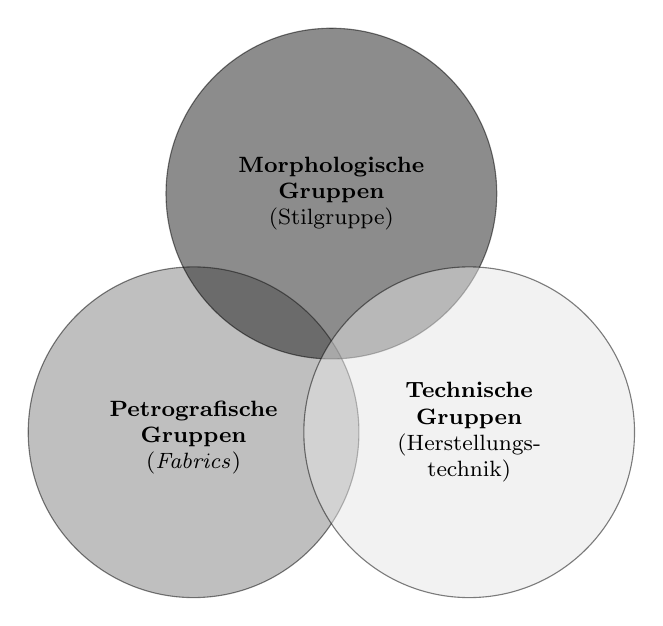
\begin{tikzpicture}[mycircle/.style={draw, circle, minimum size=4.2cm, align=center, fill=#1, opacity=0.5, text opacity=1, font = \footnotesize}] 
				\node[mycircle=black!50] {\\
					\textbf{Petrografische}\\
					\textbf{Gruppen}\\
					(\textit{Fabrics})
				};
				\node[mycircle=black!90] at (60:3.5cm) {
					\textbf{Morphologische}\\
					\textbf{Gruppen}\\
					(Stilgruppe)
				};
				\node[mycircle=black!10] at (0:3.5cm) {
					\textbf{Technische}\\
					\textbf{Gruppen}\\
					(Herstellungs-\\
					technik)
				};
				\end{tikzpicture}}}  
		\caption{Konzeption einer \enquote*{multivariaten} Analysestrategie.}
		\label{fig:KeramikherstellungAnalysestrategien_nwCongo}
	\end{subfigure}
	\caption{Analyseschritte: Schema Untersuchungsebenen bei technologischen Untersuchungen.}
	\label{fig:KeramikherstellungAnalysestrategien}
\end{figure*}

Für die Untersuchung technologischer Entscheidungsketten hat sich innerhalb der Archäologie das analytische Konzept der \textit{\mbox{chaîne} opératoire} etabliert.\footnote{Im deutschsprachigen Raum finden Analysen, die unter dem Ansatz der \textit{chaîne opératoire} durchgeführt werden, fast ausschließlich im Zusammenhang mit der Untersuchung lithischer Komplexe Anwendung. Ansätze aus dem Bereich der Analyse keramischer Inventare fehlen hier bislang vollständig, anders als innerhalb der frankophonen Archäologie \parencites[siehe][]{Gosselain.1992}{Huysecom.1994}{PeuramakiBrown.2004}{Visseyrais.2006}{Manem.2008}{Mayor.2011b}{Roux.2011}{Ard.2014}{Gomart.2014}. Außerhalb der frankophonen Archäologie sind Untersuchungen keramischer Inventare unter dem Gesichtspunkt der \textit{chaîne opératoire} noch selten \parencites[siehe][]{vanderLeeuw.1993}{PeuramakiBrown.2004}{Berg.2007}{Berg.2011}{Berg.2017}{DeLaFuente.2011}.} Konkret wird unter der \textit{chaîne opératoire} die Abfolge von Entscheidungsgängen verstanden, die sich in den zu untersuchenden Quellen materialisiert und aus diesen rekonstruierbar ist. Sie sind von unbewussten oder zufälligen Ereignissen, denen ein Objekt während seiner Herstellung oder Nutzung ausgesetzt ist, ebenso abzugrenzen wie von taphonomischen Prozessen. Letztere umfassen vornehmlich Einflüsse auf ein Objekt, nachdem es auf der Nutzung genommen und in das Bodenmilieu gelangt ist. Erste strukturelle Ansätze finden sich in den Arbeiten von André \textcites{LeroiGourhan.1964}{LeroiGourhan.1965} und Robert \textcites{Cresswell.1983}{Cresswell.1993} sowie anderer wie Pierre \textcites{Lemonnier.1992}{Lemonnier.2002}. Die Herausbildung als analytische Methode geht auf die frankophone Paläolithik-Forschung zurück \parencites[nach][]{Audouze.2002}[104f.]{BarYosef.2009}, und grundsätzlich können auch die auf dem gleichen Grundgedanken aufbauenden, mehr oder weniger parallel entwickelten Konzeptionen \textit{work chain} \parencite{Cresswell.1990} sowie \textit{operational sequence} \parencites {Perles.1992}{Dibble.1995}{Chazan.2003}[nach][105]{BarYosef.2009} synonym verwendet werden. Für die Untersuchung von keramischen Inventaren ist ein grundsätzlich \enquote*{sequenzieller} Arbeitsablauf zu empfehlen \parencites[Abb.~\ref{fig:KeramikherstellungAnalysestrategienFrankophon}; siehe][25; 26 Abb.~4]{Ard.2014}[nach][]{Roux.2007}{Roux.2010}. Dabei bilden Beobachtungen makroskopischer Spuren, die Hinweis auf die Töpferei- beziehungsweise Aufbautechnik liefern, die erste Analyseebene (Kap.~\ref{sec:Herstellung2_Toepferei}). Die sich daraus ergebenden \enquote*{Technischen Gruppen} werden in einem nächsten Arbeitsschritt auf petrografische Gemeinsamkeiten und Unterschiede hin untersucht, woraus sich \enquote*{Technisch-Petrografische Gruppen} ergeben (Kap.~\ref{sec:Herstellung2_Fabric}). Die abschließende Gliederungsebene bilden die \enquote*{klassischen} Untersuchungen morphologischer und stilistischer Elemente (Kap.~\ref{sec:Keramiksequenz}).


\section{Makrospuren und Herstellungstechniken}\label{sec:Herstellung2_Toepferei}

Die Untersuchung ur- und frühgeschichtlicher Gefäßkeramik unter Berücksichtigung von an den Stücken sichtbaren Makrospuren, welche Hinweis auf die für den Aufbau genutzte Technik geben, wurde anhand einer kleinen, aus 28 Gefäßeinheiten (GE) bestehenden Stichprobe realisiert (Tab.~\ref{tab:Makrospuren_ChaineOperatoire}).\footnote{Die an dieser Stelle zu besprechende Untersuchung wurde erst zu einem sehr späten Stadium der Arbeit als zusätzliche Analyse-Ebene hinzugefügt und konnte daher nicht mehr systematisch alle stilistisch sowie technisch (\textit{Fabrics}) untersuchten GE umfassen. Dies hatte zur Folge, dass nur in begrenztem und sehr konkretem Rahmen Fragestellungen in die Untersuchung einfließen konnten und auch keine generalisierenden Aussagen möglich waren. Die für die Auswahl an GE formulierten Fragen richteten sich an ein Inventar, das durch eine vorangegangene stilistische Analyse (Kap.~\ref{sec:Keramiksequenz}) bereits gegliedert war. Ein systematischer, dem Methodenspektrum der \textit{chaîne opératoire} verhafteter Ansatz \parencite[siehe][25f.]{Ard.2014} ließ sich aufgrund des bereits größtenteils abgeschlossenen Zustandes der Arbeit nicht mehr verwirklichen.} Ziel der Untersuchung war die Auseinandersetzung mit folgenden Kernfragen:
\begin{itemize*}
	\renewcommand\labelitemi{--}
	\item Können bereits bei einer kleinen, sich aus stilistisch beschriebenen GE zusammensetzenden Stichprobe Unterschiede in der Herstellungstechnik beobachtet werden?
	\item Lassen sich \enquote*{Technologietraditionen} identifizieren?
	\item Liefert die Untersuchung von an der Keramik beobachtbaren und auf die Herstellung zurückführbarer Makrospuren einen Beitrag für die Frage der Besiedlungsgeschichte des Arbeitsgebietes?
\end{itemize*}

\noindent Die Auswahl der GE erfolgte nach folgenden Kriterien:
\begin{itemize*}
	\renewcommand\labelitemi{--}
	\item Die GE sollten möglichst vollständig erhalten sein.
	\item Die sich durch die stilistische Untersuchung (Kap.~\ref{sec:Keramiksequenz}) abzeichnende Stilgruppen-Sequenz (Abb.~\ref{fig:Chronologiesystem}) sollte bestmöglich abgedeckt werden.
	\item Die ausgewählten Stilgruppen sollten möglichst mehrfach vertreten sein.
	\item Ein besonderes Augenmerk lag auf der Erschließung von Gemeinsamkeiten wie Unterschieden zwischen den folgenden, durch stilistische Betrachtungen erarbeiteten Gruppen:
	\begin{itemize*}
		\renewcommand\labelitemi{--}
		\item Welche Charakteristika zeigt die nur durch wenige GE belegte, älteste keramische Stilgruppe im Kongobecken, die Imbonga-Gruppe (Kap.~\ref{sec:IMB-Gr})?
		\item Welche Gemeinsamkeiten und Unterschiede ergeben sich zwischen den beiden ältesten keramischen Stilgruppen im Arbeitsgebiet: der Batalimo-Maluba-Gruppe (Kap. \ref{sec:BTM-Gr}) im nördlichen sowie der Pikunda-Munda-Gruppe (Kap.~\ref{sec:PKM-Gr}) im südlichen Teil?
		\item Zeichnet sich die schwache stilistische Variation innerhalb der Pikunda-Munda-Gruppe (Kap.~\ref{sec:PKM-Gr}) auch bei den Herstellungstechniken ab?
		\item Welche Gemeinsamkeiten und Unterschiede zeigt das stilitisch nicht mit den übrigen Funden in Einklang zu bringende Fund-Ensemble vom Fundplatz bei Flusskilometer 186 am Likwala-aux-Herbes (Kat.-Nr.~19, Kap.~\ref{sec:SHG-LKW_Einzelfunde})?
		\item Welche Gemeinsamkeiten und Unterschiede ergeben sich zwischen dem stilistisch nicht an das Material aus dem Inneren Kongobecken anzubindenden Gefäßen der Pikunda-Munda-Gruppe (Kap.~\ref{sec:PKM-Gr}) zu denen in formaler Hinsicht Ähnlichkeiten zeigenden GE der Ngombe-Gruppe (Kap.~\ref{sec:NGO-Gr})?
		\item Weisen die ältesten Stilgruppen im nördlichen Teil des Arbeitsgebietes, die Batalimo-Maluba- (Kap.~\ref{sec:BTM-Gr}) sowie die Ngbanja-Gruppe (Kap.~\ref{sec:NGB-Gr}), Unterschiede in der Herstellungstechnik auf?
		\item Welche Gemeinsamkeiten und Unterschiede ergeben sich zwischen den entlang des prospektierten Laufs des Sangha verbreiteten, die lokale Sequenz (Abb.~\ref{fig:Chronologiesystem}) abbildenden Stilgruppen: Pikunda-Munda (Kap.~\ref{sec:PKM-Gr}), Ngombe (Kap.~\ref{sec:NGO-Gr}), Mandombe (Kap.~\ref{sec:MDB-Gr}) und Konda (Kap.~\ref{sec:KON-Gr})?
		\item Welche Gemeinsamkeiten und Unterschiede ergeben sich zwischen den Stilgruppen entlang des Likwala-aux-Herbes: Pikunda-Munda (Kap.~\ref{sec:PKM-Gr}), Ebambe (Kap.\linebreak\ref{sec:EBA-Gr}) und Epena (Kap. \ref{sec:EPE-Gr})?
		\item Welche Gemeinsamkeiten und Unterschiede bestehen zwischen den entlang des Ubangi erfassten Stilgruppen: Batalimo-Maluba (Kap.~\ref{sec:BTM-Gr}), Ngbanja (Kap.\ref{sec:NGB-Gr}), Dongo (Kap.~\ref{sec:DON-Gr}) sowie Dama (Kap.~\ref{sec:DAM-Gr}) und Mbati-Ngombe (Kap.~\ref{sec:MBN-Gr})?
	\end{itemize*}
\end{itemize*}

\begin{table*}[tb]
	\centering
	\noindent\begin{minipage}[t]{\columnwidth}
{\footnotesize
\begin{sftabular}{@{}lp{.72\columnwidth}l@{}}
\toprule
\textbf{Code} & \textbf{Makro-Spur} & \textbf{Abb.}\\
\midrule
 A1 &  Spur; leicht konkav (evtl. Muschel) & \ref{NGO87-102-28_29_Makrospuren} \\
 A2a &  Spur; fein & \ref{NGB85-101-130-01_Makrospuren} \\
 A2b &  Spur; fein; eng & \ref{MUN87-2-1-1-4-2_Makrospuren} \\
 A3a &  Riefe; horizontal & \\
 A3b &  Riefe; vertikal & \ref{MUN87-1-0-2-6-2_Makrospuren} \\
 A3c &  Riefe; diagonal & \ref{LKW87-186-1_3-13_Makrospuren} \\
 & & \\ 
 B1 &  Eindruck; breit; rund (Stempel) & \\
 B2 &  Eindruck; breit; flach (Spatel/Paddel) & \\
 B3a &  Eindruck; fingerbreit & \\
 B3b &  Eindruck; klein & \ref{MUN87-2-1-1-4-2_Makrospuren} \\
 B4a &  Eindruck; tief (Werkzeugspur) & \ref{MUN87-1-0-2-6-2_Makrospuren} \\
 B4b &  Eindruck; leicht & \\
 & & \\
C1 &  Wandungsdicke; schwankend; vertikal & \ref{ITN87-103_Makrospuren} \\
C2a &  Wandungsdicke; schwankend; horizontal & \ref{MKA87-102-1_Makrospuren} \\
\bottomrule
\end{sftabular}
}
\end{minipage}\hfill
\noindent\begin{minipage}[t]{\columnwidth}
{\footnotesize
\begin{sftabular}{@{}lp{.72\columnwidth}l@{}}
\toprule
\textbf{Code} & \textbf{Makro-Spur} & \textbf{Abb.}\\
\midrule
C2b &  nicht verstrichene Wulst & \ref{DON85-101-71_Makrospuren} \\
C3a &  Wandungsdicke; schwankend (Unebenheit/Buckel) & \ref{MUN87-1-0-2-6-2_Makrospuren} \\
C3b & Wandungsdicke; schwankend; ausgedünnt & \\
C4 &  Absatz im Profil; horizontal & \\
 & & \\
D1a &  Bruch; lagiger Aufbau \parencite[siehe][140 Abb. 8.c]{Lindahl.2010} & \\
D1b & Bruch; diagonal verlaufender Aufbau \parencite[siehe][140 Abb.~8.b]{Lindahl.2010} & \\
D2a &  Bruchlinie; horizontal & \\
D2b &  Bruchlinie; diagonal & \\
D3a &  Riss; fein; horizontal & \ref{NGO87-102-27_Makrospuren} \\
D3b &  Riss; fein; spiralig aufsteigend & \ref{LKW87-186-1_3-13_Makrospuren} \\
D3c &  Riss; fein; radial & \ref{MUN87-1-0-2-1-3_Makrospuren} \\
D3d &  Riss; fein; vertikal & \ref{MIT87-103-1_Makrospuren} \\
\bottomrule
\end{sftabular}
}
\end{minipage}
	\caption{Makro-Spuren: Aufnahmeschema.}
	\label{tab:Makrospuren_Liste}
\end{table*}

\vspace{1.5em}
\noindent Die zur weiteren Begutachtung ausgewählten 28~GE spiegeln zwölf verschiedene keramische Stilgruppen wider.\footnote{In alphabetischer Reihenfolge sind die folgenden Stilgruppen vertreten: 1~GE der Batalimo-Maluba-Gruppe (Kap.~\ref{sec:BTM-Gr}; \enquote*{BTM}, 4~GE der Dama-Gruppe (Kap.~\ref{sec:DAM-Gr}; \enquote*{DAM}), 1~GE der Dongo-Gruppe (Kap.~\ref{sec:DON-Gr}; \enquote*{DON}), 3~GE der Ebambe-Gruppe (Kap.~\ref{sec:EBA-Gr}; \enquote*{EBA}), 2~GE der Epena-Gruppe (Kap.~\ref{sec:EPE-Gr}; \enquote*{EPE}), 2~GE der Imbonga-Gruppe (Kap.~\ref{sec:IMB-Gr}; \enquote*{IMB}), 2~GE der Konda-Gruppe (Kap.~\ref{sec:KON-Gr}; \enquote*{KON}), 1~GE vom Fundplatz Likwala-aux-Herbes Flusskilometer 186 (LKW), 2~GE der Mandombe-Gruppe (Kap.~\ref{sec:MDB-Gr}; \enquote*{MDB}), 2~GE der Ngbanaja-Gruppe (Kap.~\ref{sec:NGB-Gr}; \enquote*{NGB}), 2~GE der Ngombe-Gruppe (Kap.~\ref{sec:NGO-Gr}; \enquote*{NGO}) sowie 6~GE der Pikunda-Munda-Gruppe (Kap.~\ref{sec:PKM-Gr}; \enquote*{PKM}). Die genannten Stilgruppenkürzel finden sich in Tab.~\ref{tab:Makrospuren_ChaineOperatoire} wieder.\label{ftn:StilGrKurzel_UntersuchungHerstetellungstechnik}} An den in der Stichprobe enthaltenen GE konnten insgesamt 27 verschiedene Makrospuren unterschieden werden, die im Zusammenhang mit der Herstellung der Gefäße stehen (Abb.~\ref{tab:Makrospuren_Liste}). Eine systematische Aufnahme der Spuren für jede GE orientierte sich an der in dieser Arbeit genutzten Bereichs-Aufteilung für Verzierungselemente (siehe Abb.~\ref{fig:Keramik_VerzZonen}). Die beobachteten Makrospuren wurden in vier größere Gruppen unterschieden (Tab.~\ref{tab:Makrospuren_Liste}): A) Spuren, die durch Kratzen oder Schaben mit einem Werkzeug erzeugt wurden, B) Spuren, die durch das Eindrücken mit einem Werkzeug entstanden sind, C) Schwankungen der Wandung eines Gefäßes sowie D) Eigenschaften der Brüche. Die Spuren der ersten beiden Gruppen sind am häufigsten zu beobachten, repräsentieren jedoch vornehmlich die abschließende Behandlung der Oberflächen eines Gefäßes (siehe Kap.~\ref{sec:ToepfereiEthnogr}). Die Spuren der Gruppen C und D ließen sich seltener beobachten, geben jedoch Hinweise auf den internen Aufbau eines Gefäßes und damit die genutzte Herstellungstechnik.

\begin{figure*}[p]
	\centering
	\begin{subfigure}{\textwidth}
		\centering
		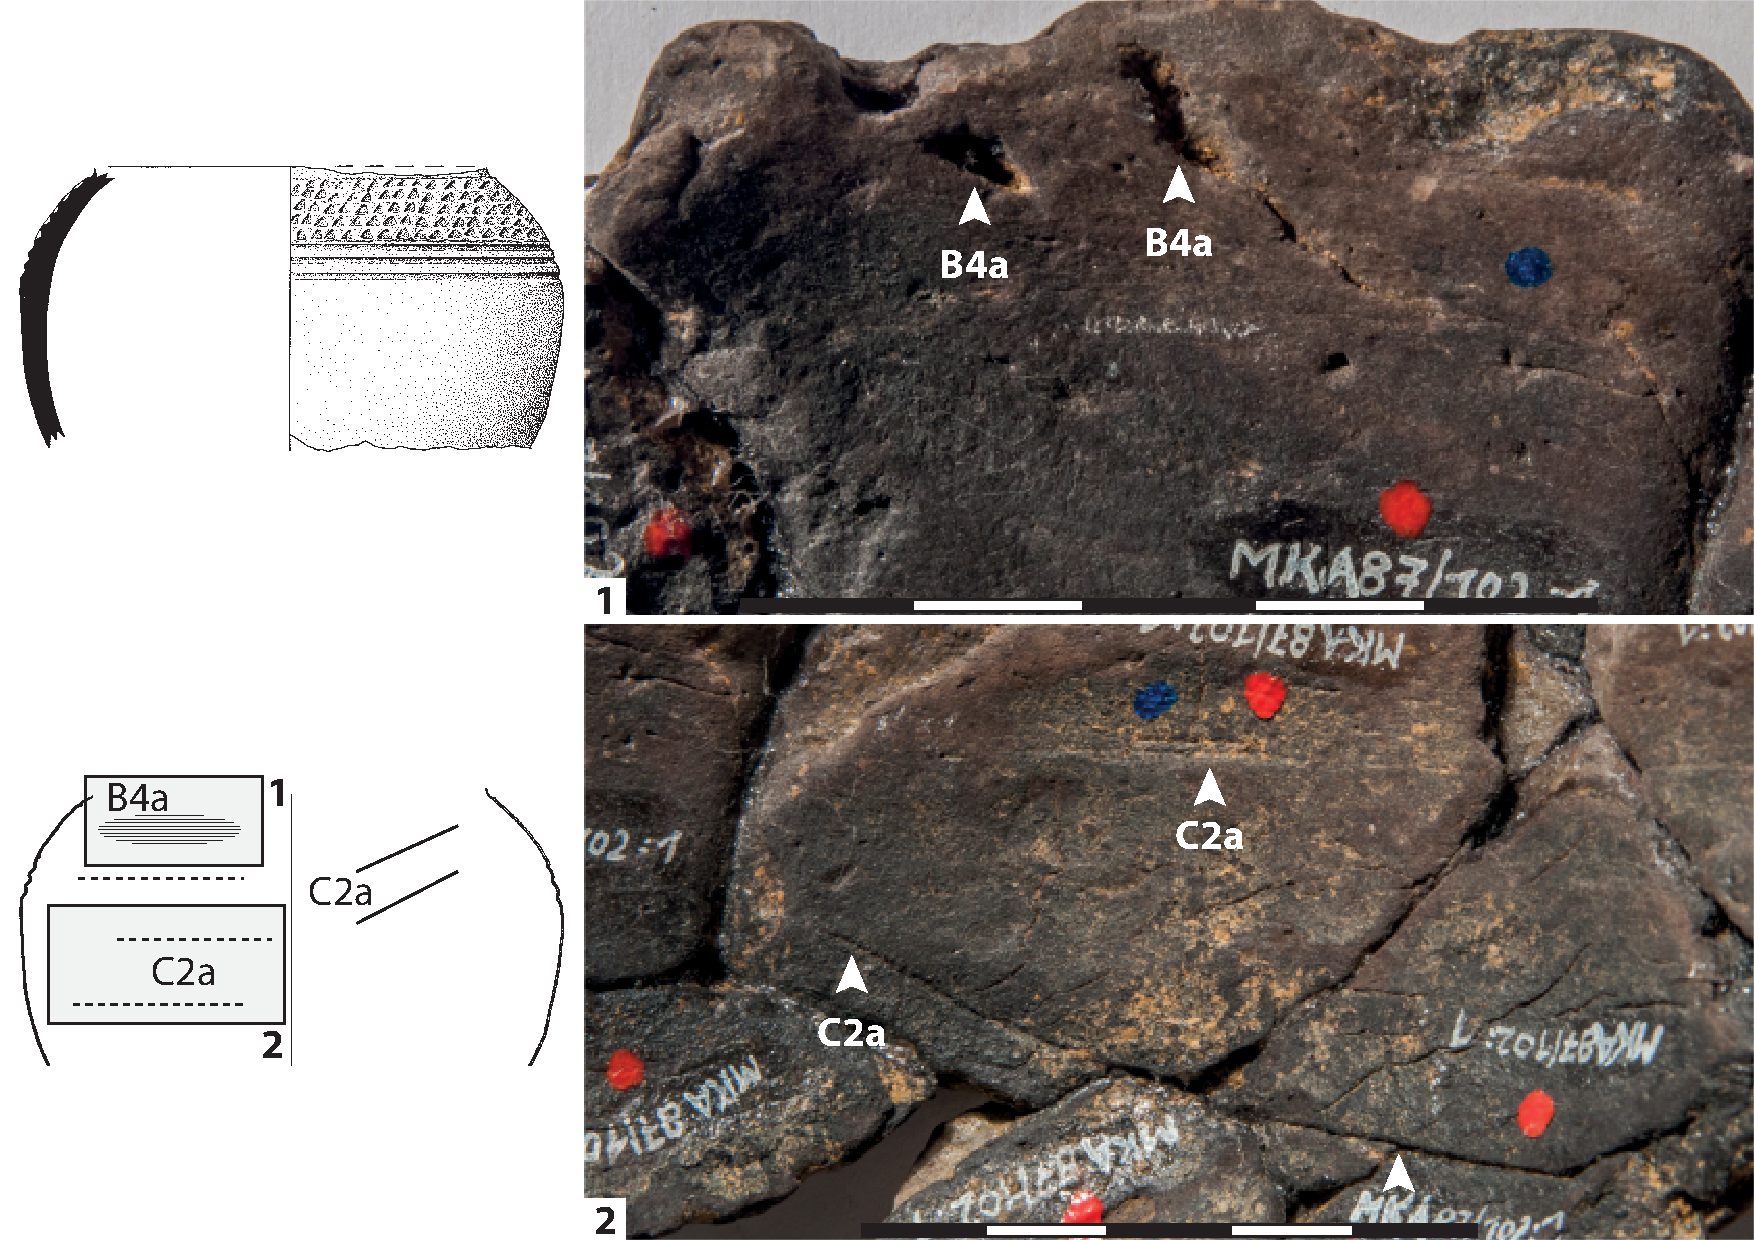
\includegraphics[height = .45\textheight]{misc/KeramikHerstellungstechnik/Gef/MKA87-102-1.pdf}
		\caption{Mobaka (Fpl.~246): Obj.~MKA~87/102:1 (Taf.~39.5).\vspace{1em}}
		\label{MKA87-102-1_Makrospuren}
	\end{subfigure}
	\begin{subfigure}{\textwidth}
		\centering
		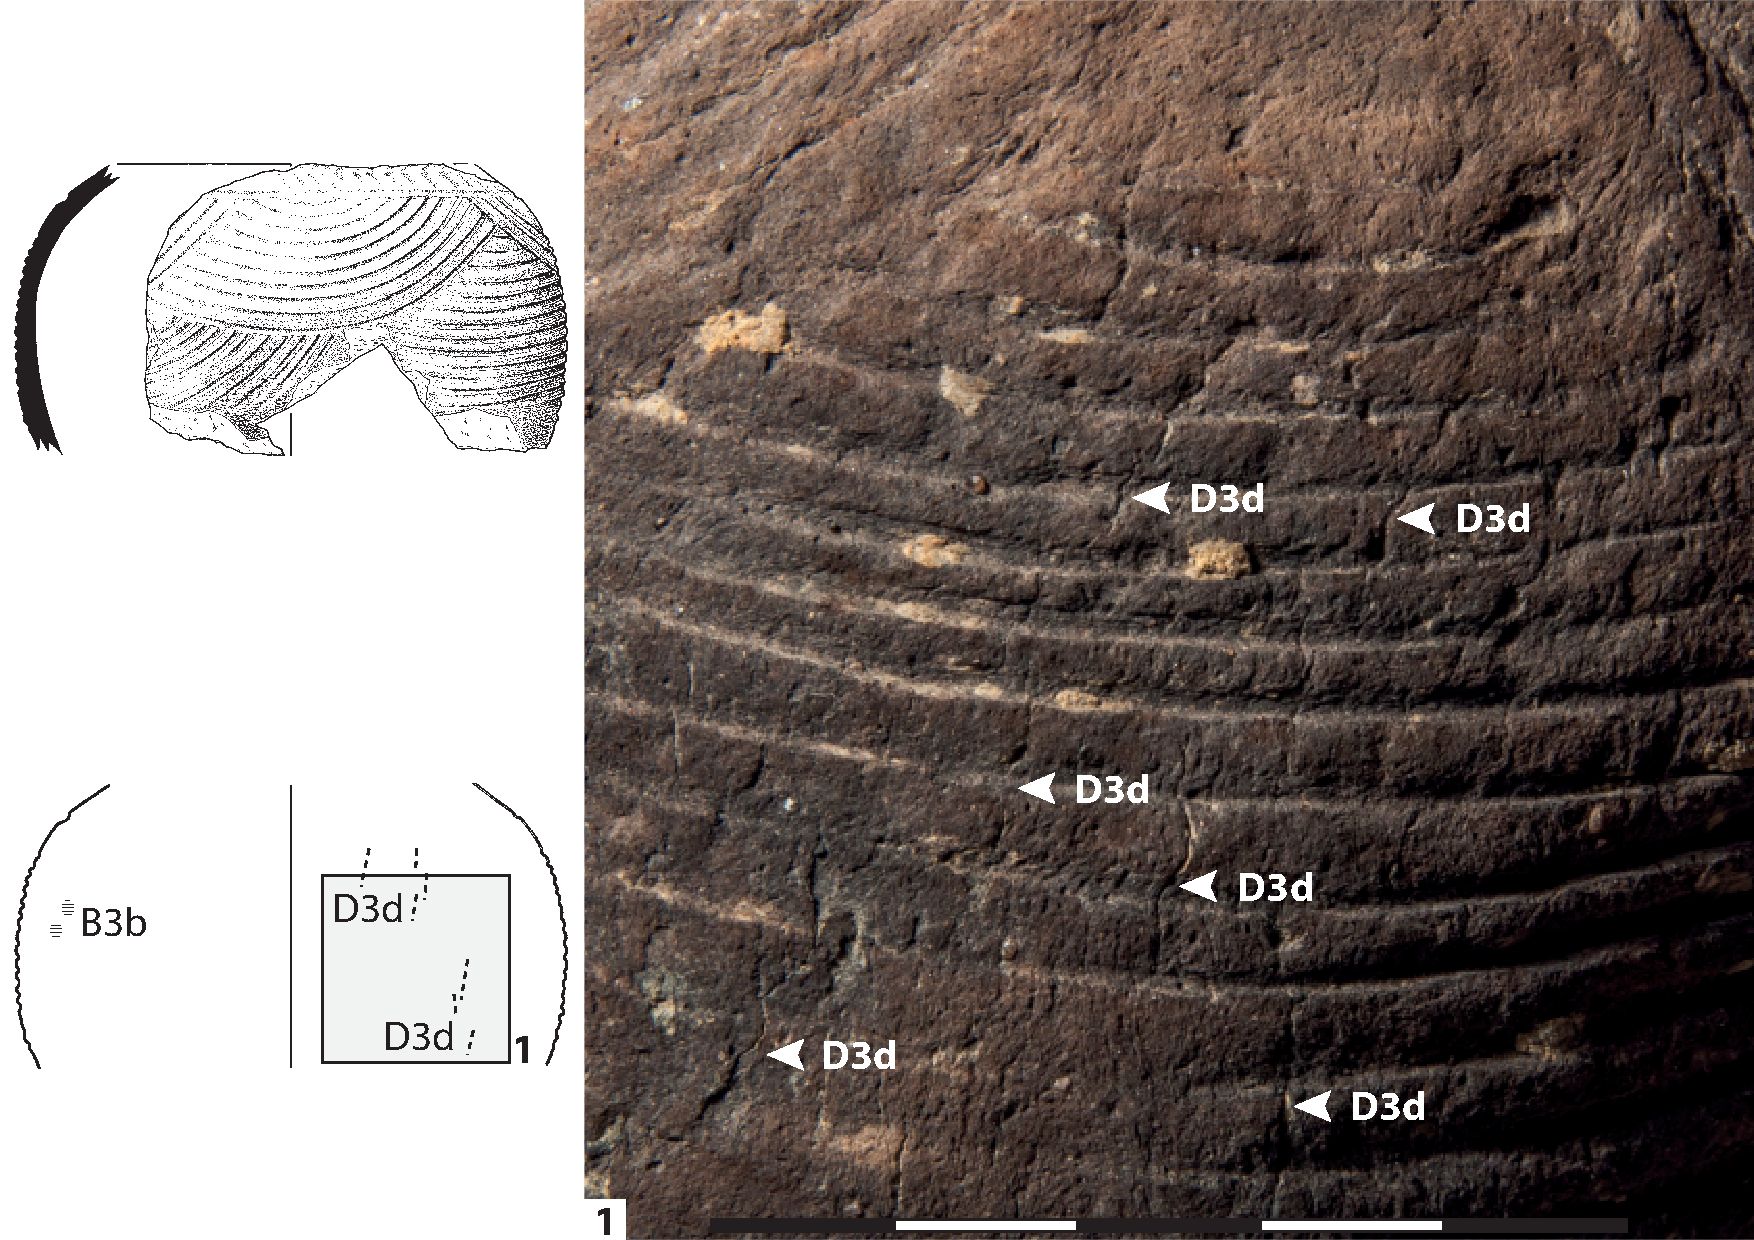
\includegraphics[height = .45\textheight]{misc/KeramikHerstellungstechnik/Gef/MIT87-103-1.pdf}
		\caption{Mitula (Fpl.~251): Obj.~MIT~87/103:1 (Taf.~42.10).}
		\label{MIT87-103-1_Makrospuren}
	\end{subfigure}
	\caption{Makrospuren: Aufnahme und Details.}
\end{figure*}

Stellvertretend für die ältesten im Arbeitsgebiet vertretenen Stilgruppen wurden Stücke aus ausgegrabenen und gut datierten Komplexen ausgewählt. Die beiden der Imbonga-Gruppe (Kap. \ref{sec:IMB-Gr}) zuweisbaren Stücke aus Mobaka und Mitula liefern einen ersten Einblick in die mit den Herstellungsprozessen in Zusammenhang stehenden Makrospuren dieser vor allem weiter östlich verbreiteten, frühesten Keramik der Region. An der Außenseite des Gefäßes aus Mobaka (Abb.~\ref{MKA87-102-1_Makrospuren}) finden sich im Bereich der größten Weite flache, diagonal aufsteigende rippenartige Erhebungen, die zu einer schwankenden Wandungsdicke führen (C2a). An der Innenseite lassen sich im Bereich des Gefäßbauches horizontale, flache Verdickungen und Eintiefungen beobachten, die ebenfalls zu Schwankungen der Wandungsstärke entlang des Profils führen (Abb.~\ref{MKA87-102-1_Makrospuren}.2:~C2a). Unterhalb des Schulter-Umbruches befinden sich bis auf etwa die halbe Wandungsdicke reichende Eintiefungen (Abb.~\ref{MKA87-102-1_Makrospuren}.1:~B4a), die möglicherweise auf die Verbindung einzeln gefertigter Abschnitte hinweisen. Die Brüche lassen eine plattige beziehungsweise parallel zur Wandung verlaufende Struktur erkennen (D1a), die auf einen Aufbau durch Treiben hindeutet \parencite[siehe Kap.~\ref{sec:ToepfereiEthnogr};][140 Abb. 8.c--d]{Lindahl.2010}. Die Außenseite des Gefäßes aus Mitula weist einige feine, vertikal verlaufende Bündel aus Rissen auf (Abb.~\ref{MIT87-103-1_Makrospuren}.1:~D3d). An der Innenseite sind neben vereinzelten leicht inselartigen Erhebungen und Eintiefungen keine Makrospuren zu erfassen. 

%\addtocounter{figure}{-1}
\begin{figure*}[p]
	\centering
	\begin{subfigure}{\textwidth}
		%\setcounter{subfigure}{2}
		\centering
		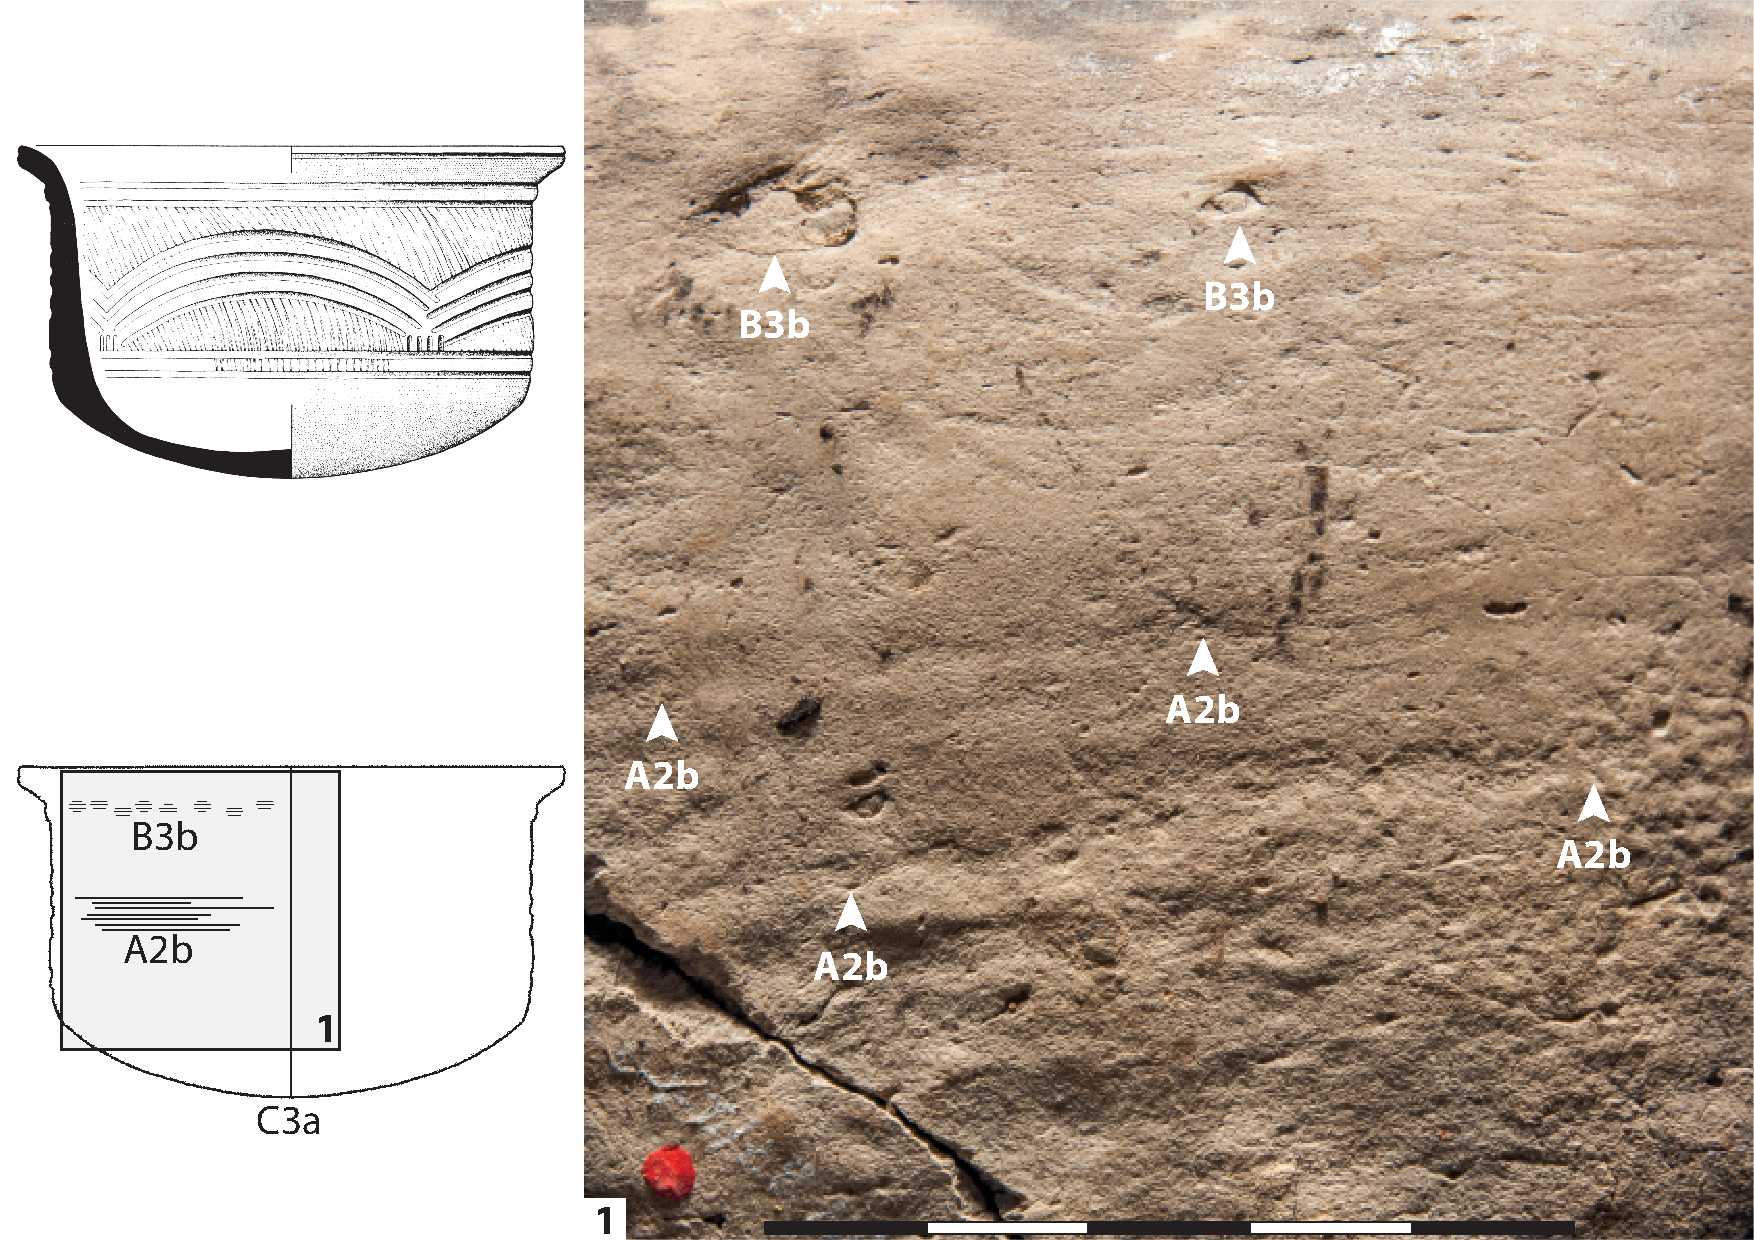
\includegraphics[height = .45\textheight]{misc/KeramikHerstellungstechnik/Gef/MUN87-2-1-1-4-2.pdf}
		\caption{Munda (Fpl.~304): Obj.~MUN~87/2-1-1-4:2 (Taf.~91.1).\vspace{1em}}
		\label{MUN87-2-1-1-4-2_Makrospuren}
	\end{subfigure}
	\begin{subfigure}{\textwidth}
		\centering
		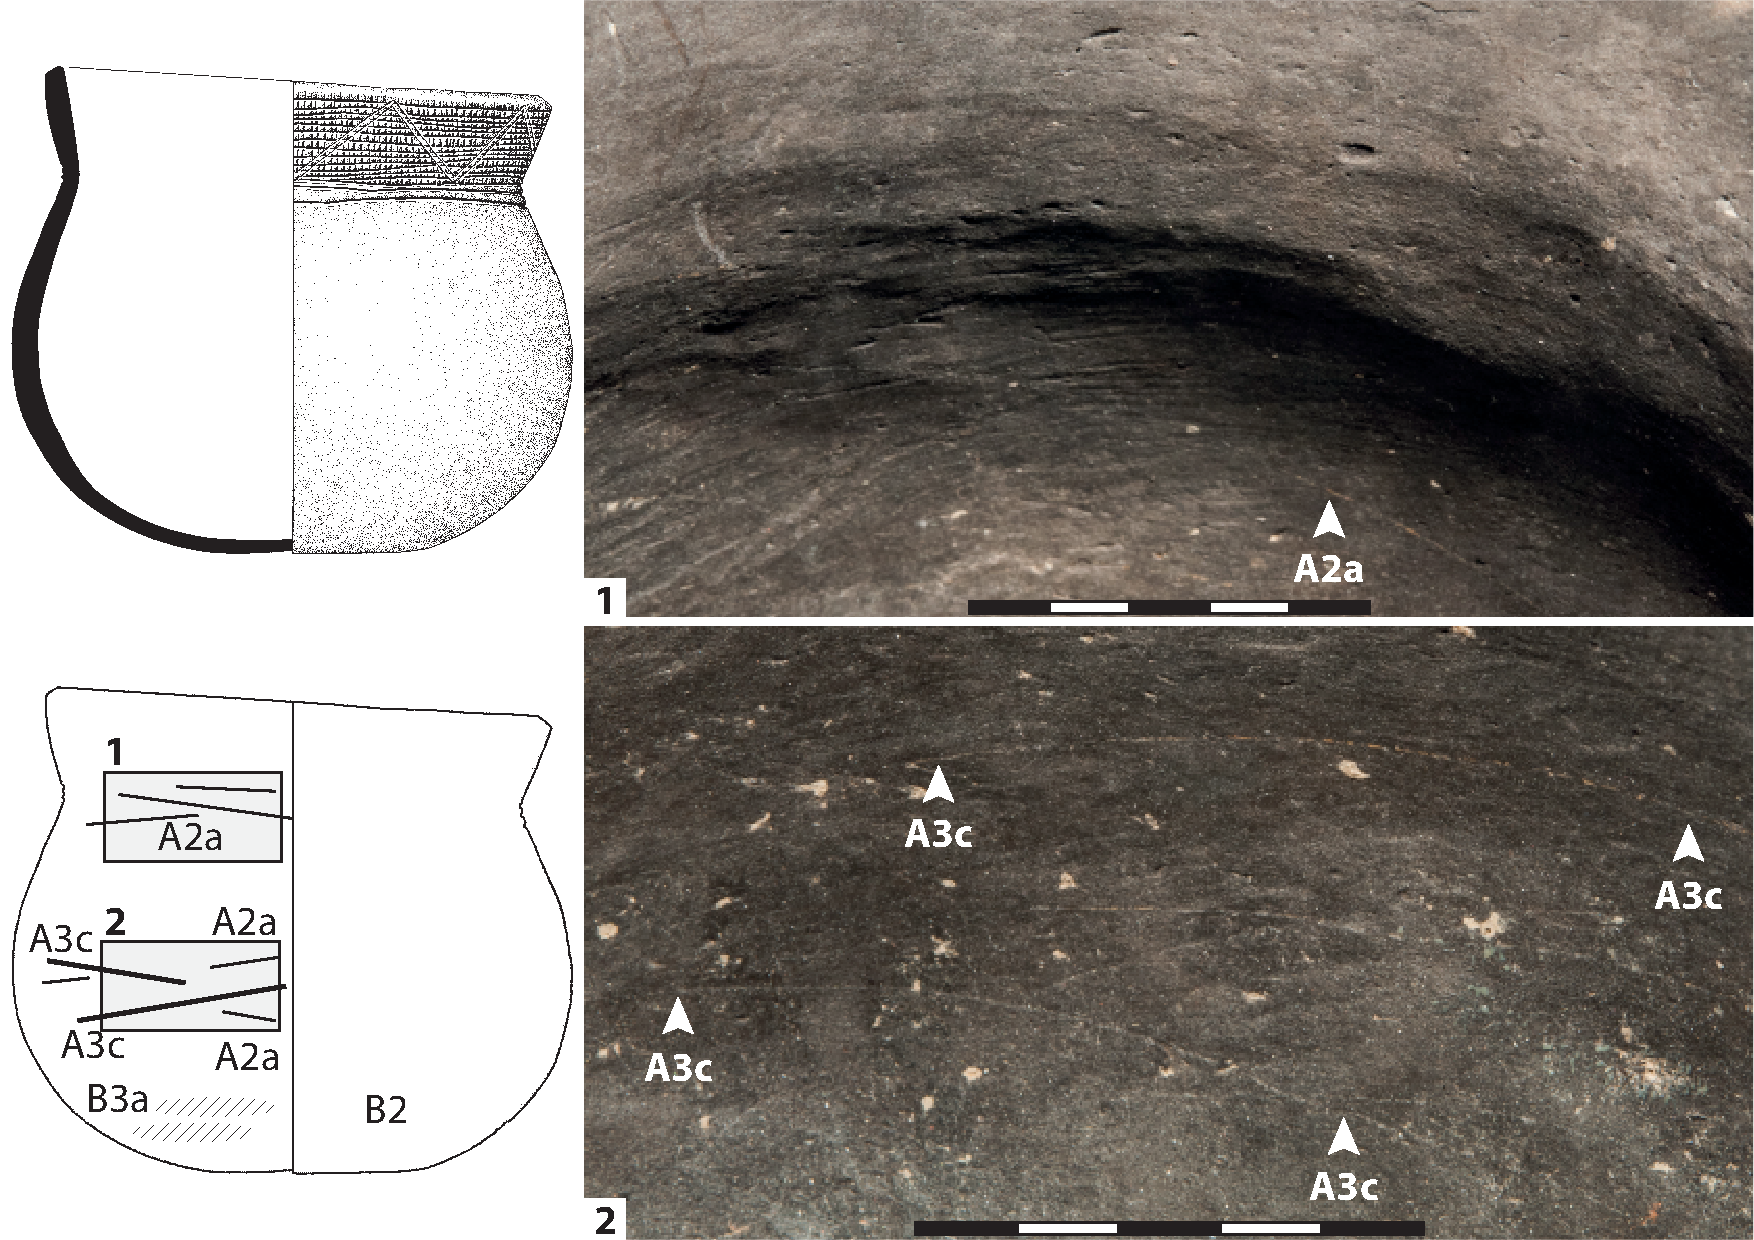
\includegraphics[height = .45\textheight]{misc/KeramikHerstellungstechnik/Gef/MUN87-2-1-3-10_Gef10.pdf}
		\caption{Munda (Fpl.~304): Obj.~MUN~87/2-1-3:10 (Taf.~93.3).}
		\label{MUN87-2-1-3-10_Makrospuren}
	\end{subfigure}
	\caption{Makrospuren: Aufnahme und Details.}
\end{figure*}

Zwei Gefäße aus dem in Pikunda am mittleren Sangha ausgegrabenen Befund PIK~87/1 (Kat.-Nr.~8) sowie je zwei weitere Gefäße aus den in Munda am oberen Likwala-aux-Herbes ergrabenen Gruben MUN~87/2-1-1 (Kat.-Nr.~16) sowie MUN~87/2-1-3 (Kat.-Nr.~17) stehen stellvertretend für das Formenspektrum der Pikunda-Munda-Gruppe (Kap.~\ref{sec:PKM-Gr}). Aufgrund seiner flächigen Verzierung lassen sich an der Außenseite eines aus dem Befund PIK~87/1 in Pikunda am Sangha stammenden Gefäßes der Pikunda-Munda-Gruppe (Kat.-Nr.~8; Taf.~44.3) keine Makrospuren erkennen. An der Innenseite zeigen sich im oberen Teil lediglich sehr feine, etwa nur 5\,mm voneinander entfernt sitzende Glättspuren (A2b), während der untere Teil feine spiralig beziehungsweise diagonal aufsteigende Risse zeigt (D3b; siehe Abb.~\ref{LKW87-186-1_3-13_Makrospuren}). Die Bruchlinien der einzelnen Fragmente verlaufen vorwiegend diagonal und folgen den feinen Rissen (D2b). Im Bereich des rund ausgeführten Gefäßbodens ließen sich keine Makrospuren beobachten. Die Bruch-Struktur des Stückes ist bis knapp unterhalb des Randes plattig beziehungsweise parallel zur Wandung (D1a; siehe ebd. 140 Abb. 8.c--d). Eine solche interne Strukturierung kann als Hinweis auf eine Herstellung durch Treiben angesehen werden. Im Randbereich hingegen verläuft die innere Struktur des Scherbens eher diagonal und deutet auf eine Aufbautechnik hin (D1b; siehe Kap.~\ref{sec:ToepfereiEthnogr}; ebd. 140 Abb. 8.b). Ein aus mehreren Fragmenten zusammensetzbares, ebenfalls aus dem Befund in Pikunda stammendes Gefäß (Taf.~45.1) weist eine vollständig geglättete Oberfläche auf, die keine Makrospuren zeigt. Im Schulterbereich ist eine leichte Verdickung der Wandung zu beobachten und das einzige auffällige Merkmal ist die Strukturierung der Brüche. Es zeigt diagonale Bruch-Facetten (D2d) und innerhalb der Bruchflächen lässt sich eine diagonale Strukturierung erkennen (D1b). Eine der Pikunda-Munda-Schalen aus dem Befund MUN~87/2-1-1 in Munda am Likwala-aux-Herbes (Kat.-Nr.~16) weist unterhalb des Randes eine mehr oder weniger horizontale Reihe kleiner runder bis leicht ovaler Löcher beziehungsweise Eindrücke auf (Abb.~\ref{MUN87-2-1-1-4-2_Makrospuren}.1:~B3b). Die Innenseite der Wandung zeigt vereinzelt eng beieinander sitzende Glättspuren (Abb.~\ref{MUN87-2-1-1-4-2_Makrospuren}.1:~A2b) und der für die Schale der Pikunda-Munda-Gruppe so charakteristische Profilknick zwischen Wandung und Boden ist im Bruch eine zusätzlich aufgebrachte Wulst sichtbar. Höchstwahrscheinlich markiert der Knick einen Wechsel in der Aufbautechnik. Der rund ausgeführte Boden ist mittig deutlich verdickt (C3a), was auf überschüssiges Material beim möglicherweise finalen Verschließen der Bodenpartie hinweisen kann. Die Innenseite eines zweiten Gefäßes (Taf.~91.5) zeigt ebenfalls flächige, eng beieinander sitzende, feine Glättspuren (A2b). Der Boden hingegen ist glatt und mittig ebenfalls leicht verdickt (C3a). Überdies zeigen sich im Bodenbereich sternförmig zum Zentrum zulaufende Risse (D3c). Zusammengenommen deuten diese Merkmale an, dass der Gefäßboden erst zum Ende des Formgebungsprozesses geschlossen wurde. Im Bruch lässt sich eine plattige, parallel zur Wandung verlaufende innere Struktur des Gefäßes (D1a) beobachten, die als Anzeiger für einen Aufbau durch Treiben angesehen werden kann (siehe Kap.~\ref{sec:ToepfereiEthnogr}; ebd. 140 Abb. 8.c--d). Ein Gefäß mit geschweifter Wandung und ausbiegendem Rand aus der benachbarten Grube MUN~87/2-1-3 (Kat.-Nr.~17) zeigt im unteren Bereich außen deutlichen Wurzelfraß. Auffällig ist eine leichte Facettierung des Gefäßunterteils (B2), die eine Formgebung unter Zuhilfenahme eines Töpferpaddels möglich erscheinen lässt. Die Wandungsdicke im Bereich des rund ausgeführten Bodens ist teilweise deutlich ausgedünnt (C3b), was ebenfalls als Hinweis darauf gewertet werden, dass der Boden erst gegen Ende der Formgebung geschlossen wurde, wobei nicht ausreichend Material zur Verfügung stand. An der Innenseite zeigen sich im Bereich des Halsansatzes leicht diagonale bis horizontale feine Glättspuren (Abb.~\ref{MUN87-2-1-3-10_Makrospuren}.1:~A2a). Im Bereich des größten Umfangs sind innen bogenförmige, mehr oder minder horizontal verlaufende feine Glättrillen zu sehen (Abb.~\ref{MUN87-2-1-3-10_Makrospuren}.2:~A3c). Ebenfalls fallen in dieser Bereich leichte, spiralig aufsteigende Absätze auf (C2a). Im Bereich des Gefäßbodens zeigen sich innen etwa fingerbreite leichte Eindrücke (B3a), die -- wie auch im Fall der Außenseite -- zu einer leichten Facettierung führen. Ein zweites Gefäße, eine der klassischen Pikunda-Munda-Schalen aus dem selben Befund, weist ebenfalls eine stark angelöste und erodierte Oberfläche auf (Taf.~93.1). Nur noch an wenigen Stellen sind Makrospuren sichtbar. Im oberen Gefäßteil zeigen sich innen sehr feine und eng sitzende Glättspuren (A2b). Im unteren Gefäßteil beziehungsweise am Bodensatz schwankt die Wandungsdicke leicht; es bilden sich leicht erhabene und eingetiefte Zonen aus (C2a). Die Wandungsdicke im Bodenbereich ist auffällig gering (C3b). Dies kann darauf hindeuten, dass der Boden erst am Ende geschlossen wurde.

%\addtocounter{figure}{-1}
\begin{figure*}[p]
	\centering
	\begin{subfigure}{\textwidth}
		%\setcounter{subfigure}{4}
		\centering
		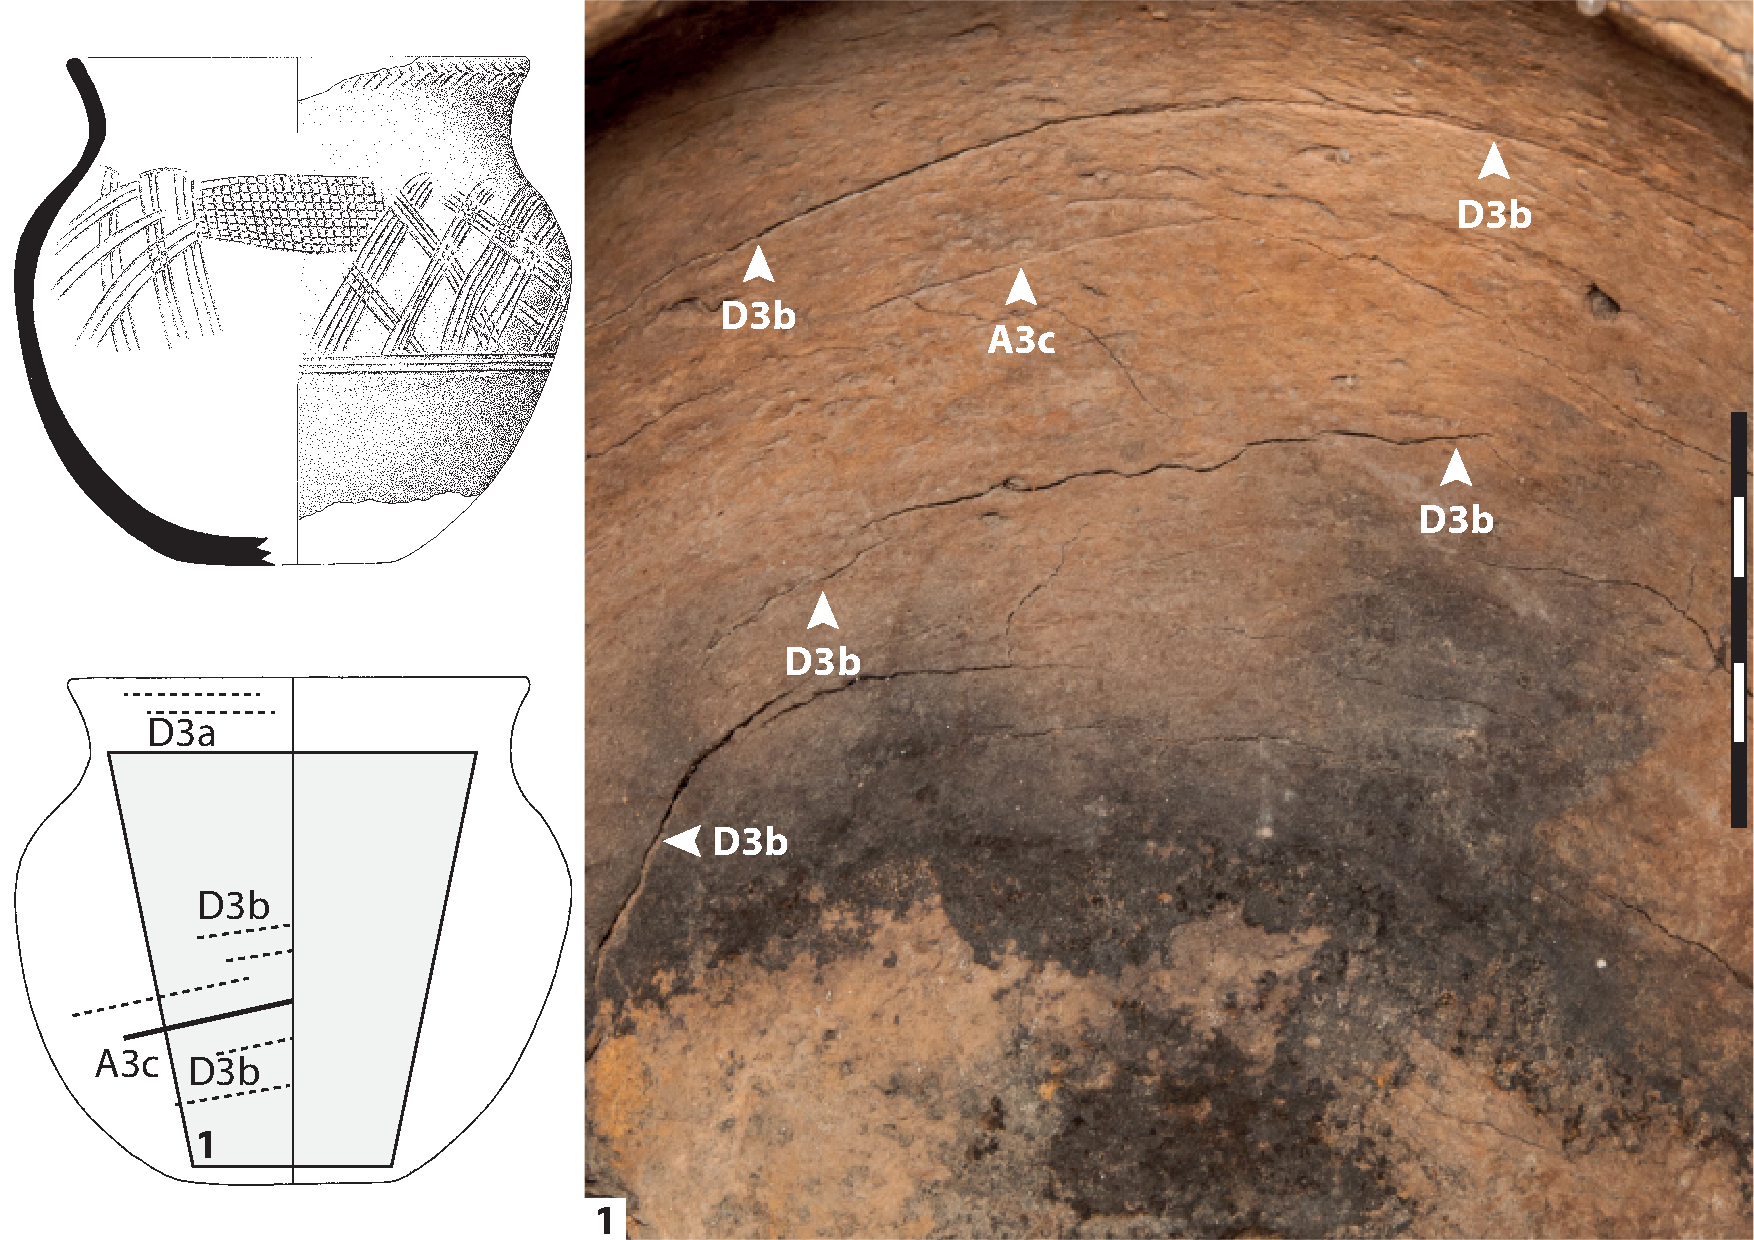
\includegraphics[height = .45\textheight]{misc/KeramikHerstellungstechnik/Gef/LKW87-186-1_3-13.pdf}
		\caption{Likwala-aux-Herbes, Flusskilometer 186 (Fpl.~291): Obj.~LKW~87/186-1:3--13 (Taf.~76.1).\vspace{1em}}
		\label{LKW87-186-1_3-13_Makrospuren}
	\end{subfigure}
	\begin{subfigure}{\textwidth}
		\centering
		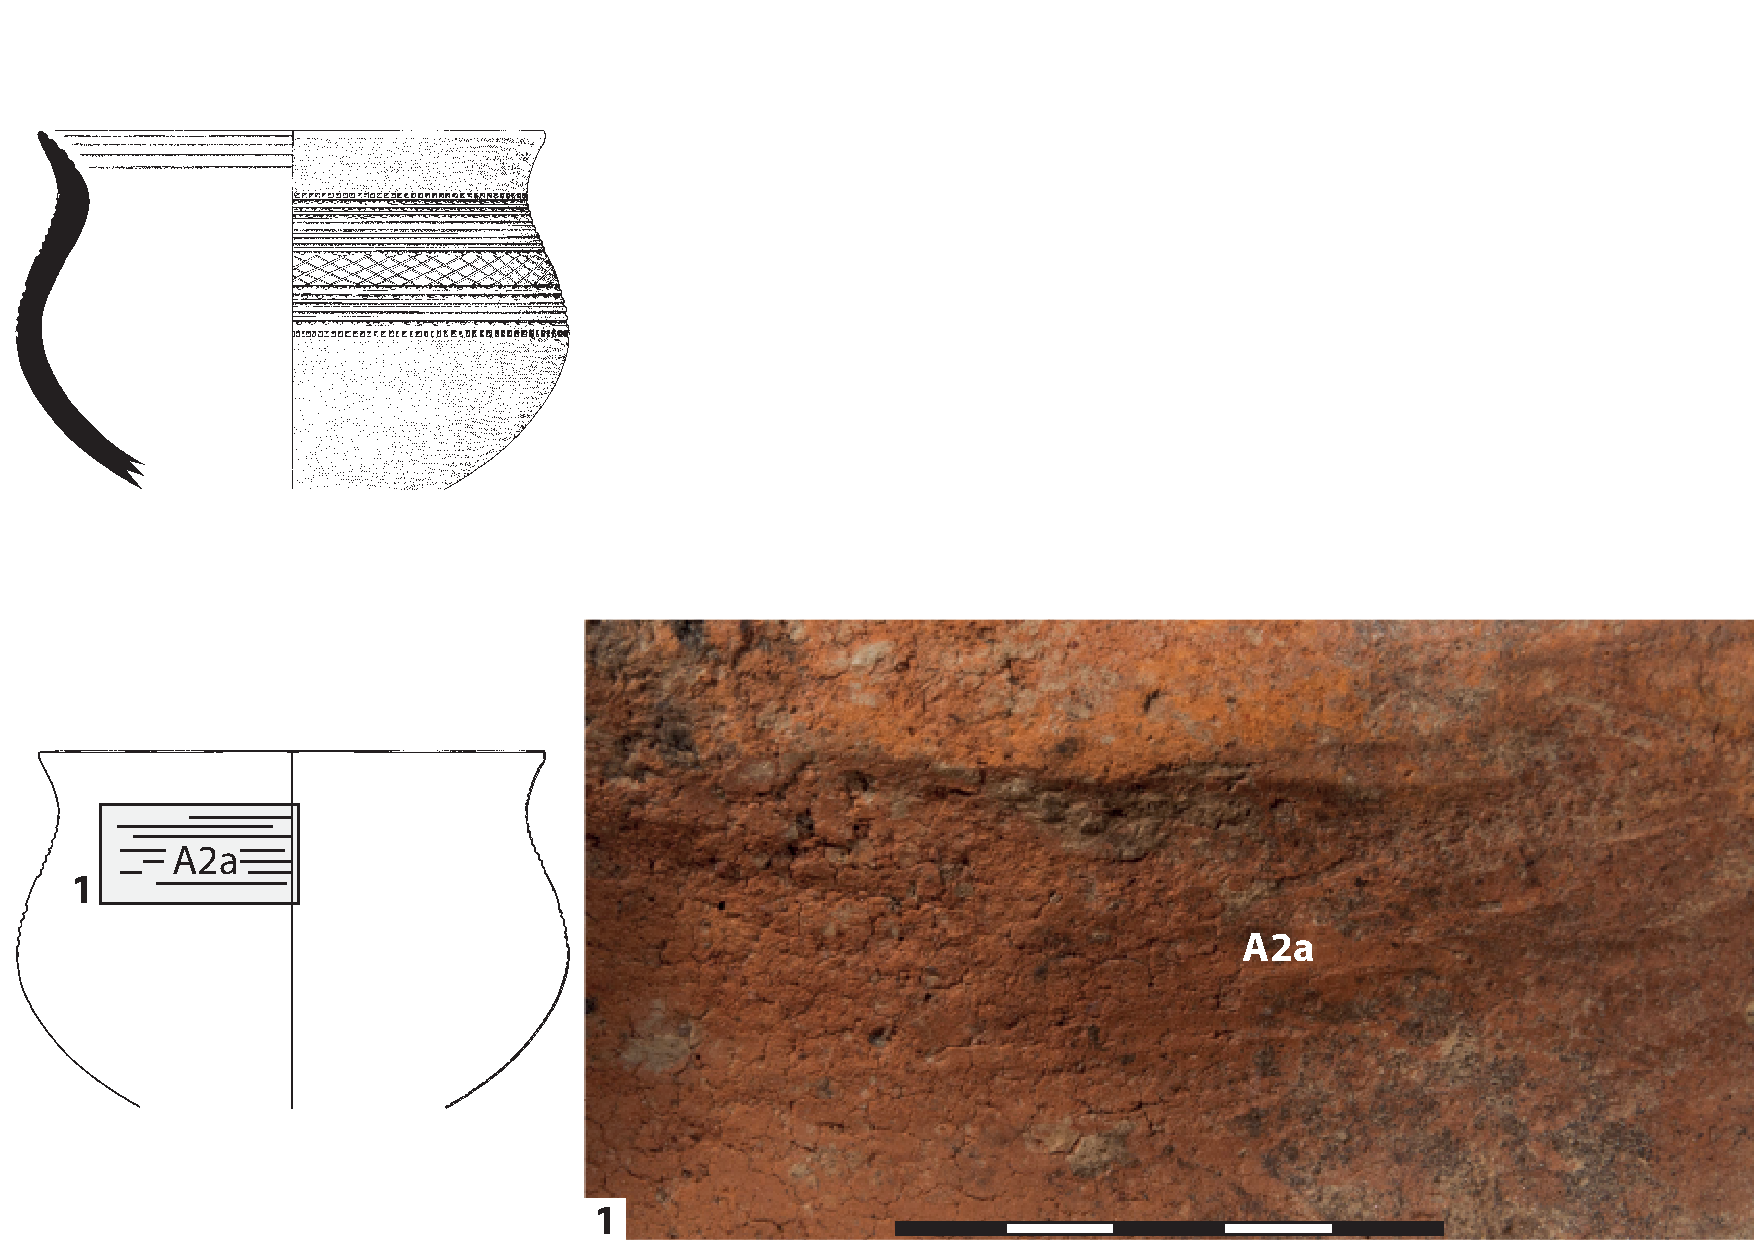
\includegraphics[height = .45\textheight]{misc/KeramikHerstellungstechnik/Gef/NGB85-101-130.pdf}
		\caption{Ngbanja (Fpl.~199): Obj.~NGB~85/101:131 (Taf.~7.6).}
		\label{NGB85-101-130-01_Makrospuren}
	\end{subfigure}
	\caption{Makrospuren: Aufnahme und Details.}
\end{figure*}

Ein Gefäße aus dem am Flusskilometer 186 am Likwala-aux-Herbes erfassten Grubeninventar (Kat.-Nr.~19) zeigt im Randbereich  feine, horizontale Glättspuren (A2) sowie Risse (Abb.~\ref{LKW87-186-1_3-13_Makrospuren}.1:~D3a). Den gesamten Gefäßbauch durchziehen innen spiralig aufsteigende, lange und tiefe Risse (Abb.~\ref{LKW87-186-1_3-13_Makrospuren}.1:~D3b). In gleicher Orientierung lassen sich auch einige Glättriefen (Abb.~\ref{LKW87-186-1_3-13_Makrospuren}.1:~A3c) beobachten. 
% Diese Risse könnten einen Hinweis darauf geben, dass das Gefäß durch Modellieren\todo{?}{} hergestellt wurde, wobei angenommen werden muss, dass der Rohling dabei beständig gedreht wurde.

%\addtocounter{figure}{-1}
\begin{figure*}[p]
	\centering
	\begin{subfigure}{\textwidth}
		%\setcounter{subfigure}{8}
		\centering
		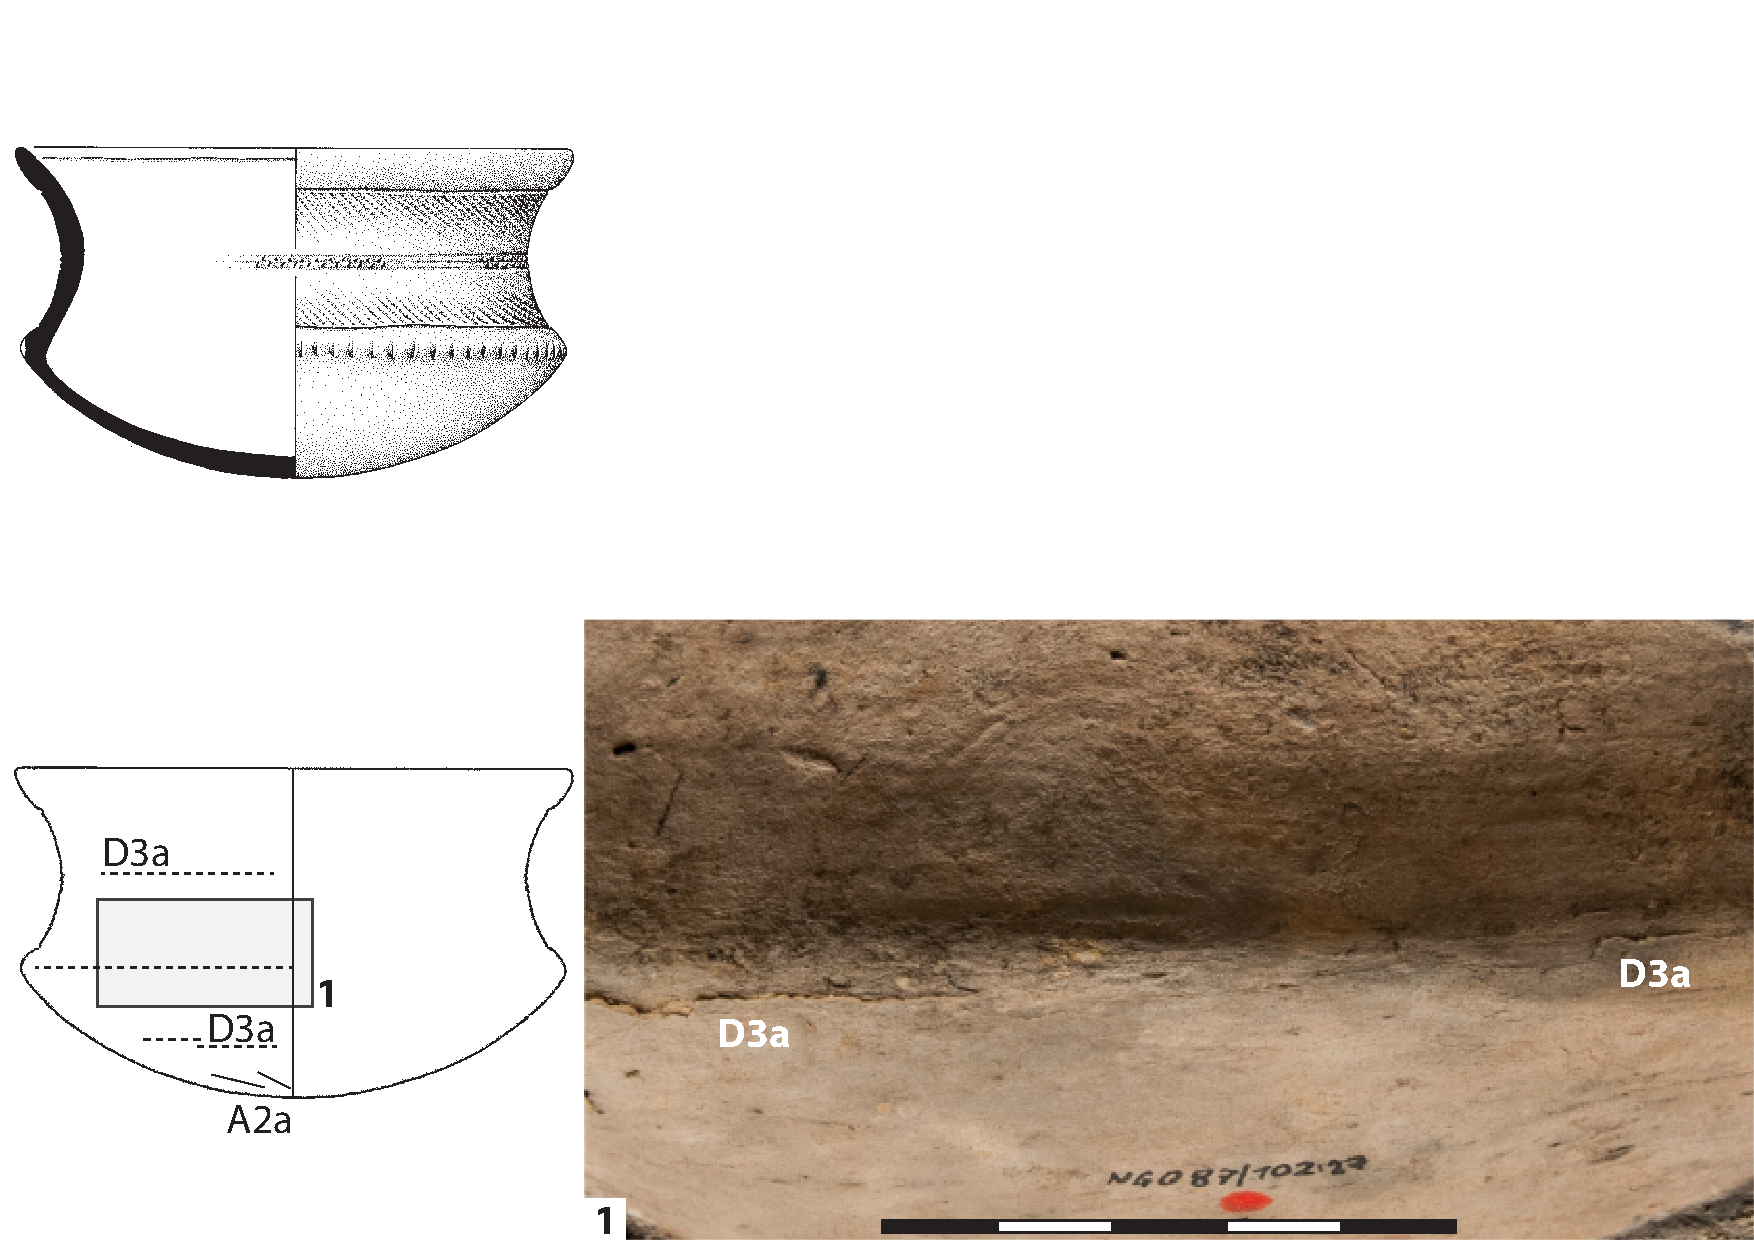
\includegraphics[height = .45\textheight]{misc/KeramikHerstellungstechnik/Gef/NGO87-102-27.pdf}
		\caption{Ngombe (Fpl.~252): Obj.~NGO~87/102:27 (Taf.~42.16).\vspace{1em}}
		\label{NGO87-102-27_Makrospuren}
	\end{subfigure}
	\begin{subfigure}{\textwidth}
		\centering
		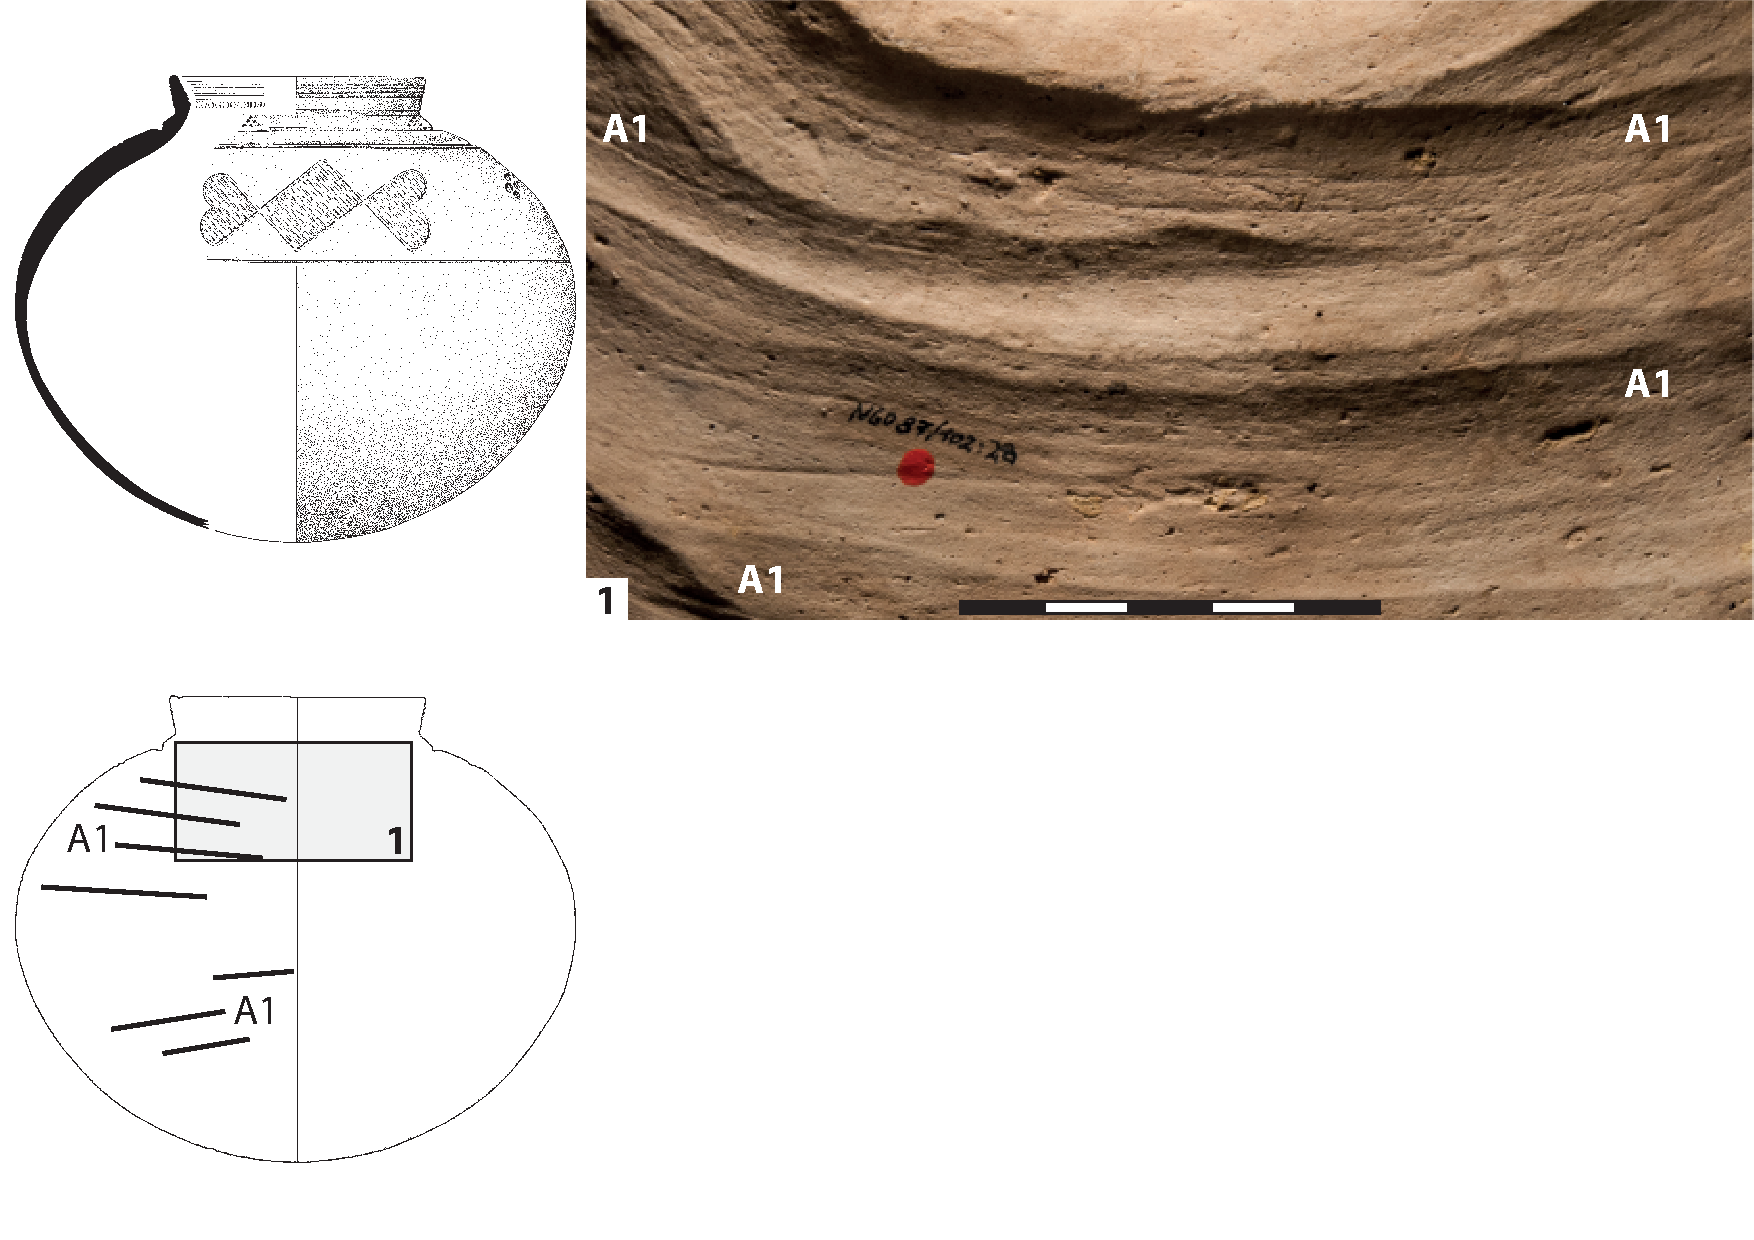
\includegraphics[height = .45\textheight]{misc/KeramikHerstellungstechnik/Gef/NGO87-102-28_29.pdf}
		\caption{Ngombe (Fpl.~252): Obj.~NGO~87/102:28--29 (Taf.~43.1).}
		\label{NGO87-102-28_29_Makrospuren}
	\end{subfigure}
	\caption{Makrospuren: Aufnahme und Details.}
\end{figure*}

Die Keramik der Ngombe-Gruppe (Kap.~\ref{sec:NGO-Gr}) ist durch zwei formal durchaus unterschiedliche Gefäße repräsentiert. Beide stammen aus dem für die Beschreibung der Stilgruppe entscheidenden Befund in Ngombe am mittleren Sangha (Kat.-Nr.~11). Die Keramik dieser Stilgruppe weist formal starke Tendenzen zu Material aus dem Inneren Kongobecken auf, vor allem der Longa-Gruppe \parencite[121--128]{Wotzka.1995}. Die erfassten Makrospuren einer Knickwandschale umfassen im oberen Gefäßteil sowie nahe des Bodens feine horizontale Risse (D3a) sowie im Bereich des Bodens feine spiralige Glättspuren (Abb.~\ref{NGO87-102-27_Makrospuren}.1:~A2a). Der Boden des Gefäßes weist eine Durchlochung auf und wurde eventuell am Ende des Aufbaues geschlossen oder ausgearbeitet, wie die spiralige Spuren im Bodenbereich andeuten. Das stark bauchige, zweite Gefäße weist innen deutliche Glättspuren eines konkaven Werkzeugs auf, die regelhaft etwa 20--25\,mm auseinander liegen (Abb.~\ref{NGO87-102-28_29_Makrospuren}.1:~A1). Zudem verlaufen die Bruchlinien des Gefäßes vor allem horizontal (D2a), was erfahrungsgemäß im Zusammenhang mit in Aufbautechnik hergestellter Keramik zu beobachten ist, bei der die Nahtbereiche zwischen den einzelnen Wülsten strukturelle Schwachstellen bilden.

Ein Gefäß der Batalimo-Maluba-Gruppe (Taf.~26.12), der ältesten entlang des Ubangi belegten keramischen Stilgruppe (Kap.~\ref{sec:BTM-Gr}), zeigt lediglich am Übergang von der Gefäßschulter zum Hals sowie dem größten Bauchdurchmesser einige wenige, leichte Glättspuren (A2a). Der Übergang zwischen Schulter und Hals ist innen durch eine scharfe Kante markiert, was andeutet, dass hier zwei separate Teile zusammengefügt wurden. Zwei GE der der Batalimo-Maluba-Gruppe stilistisch sehr nah stehenden Keramik, die vor allem entlang des mittleren Ubangi zu finden ist und als Ngbanja-Gruppe systematisiert ist (Kap.~\ref{sec:NGB-Gr}), wurden ebenfalls ausgewählt. Ein Gefäß aus dem eponymen Fundort Ngbanja weist innen im Bereich der Gefäßschulter sowie oberhalb der größten Gefäßweite einige eng sitzende leichte Glättspuren auf (Abb.~\ref{NGB85-101-130-01_Makrospuren}.1:~A2b), während der untere Teil gänzlich glatt ist. An einem zweiten, aus der gleichen Fundstelle stammenden Gefäß (Taf.~6.8) finden sich innen bis auf einige leichte Riefen im Bereich der größten Gefäßweite keinerlei Makrospuren. Die Keramik der Ngbanja-Gruppe zeichnet sich, wie auch die Batalimo-Maluba-Keramik, durch nur sehr wenige makroskopisch sichtbare Spuren aus, die Hinweise auf die Herstellung liefern können.

%\addtocounter{figure}{-1}
\begin{figure*}[p]
	\centering
	\begin{subfigure}{\textwidth}
		%\setcounter{subfigure}{6}
		\centering
		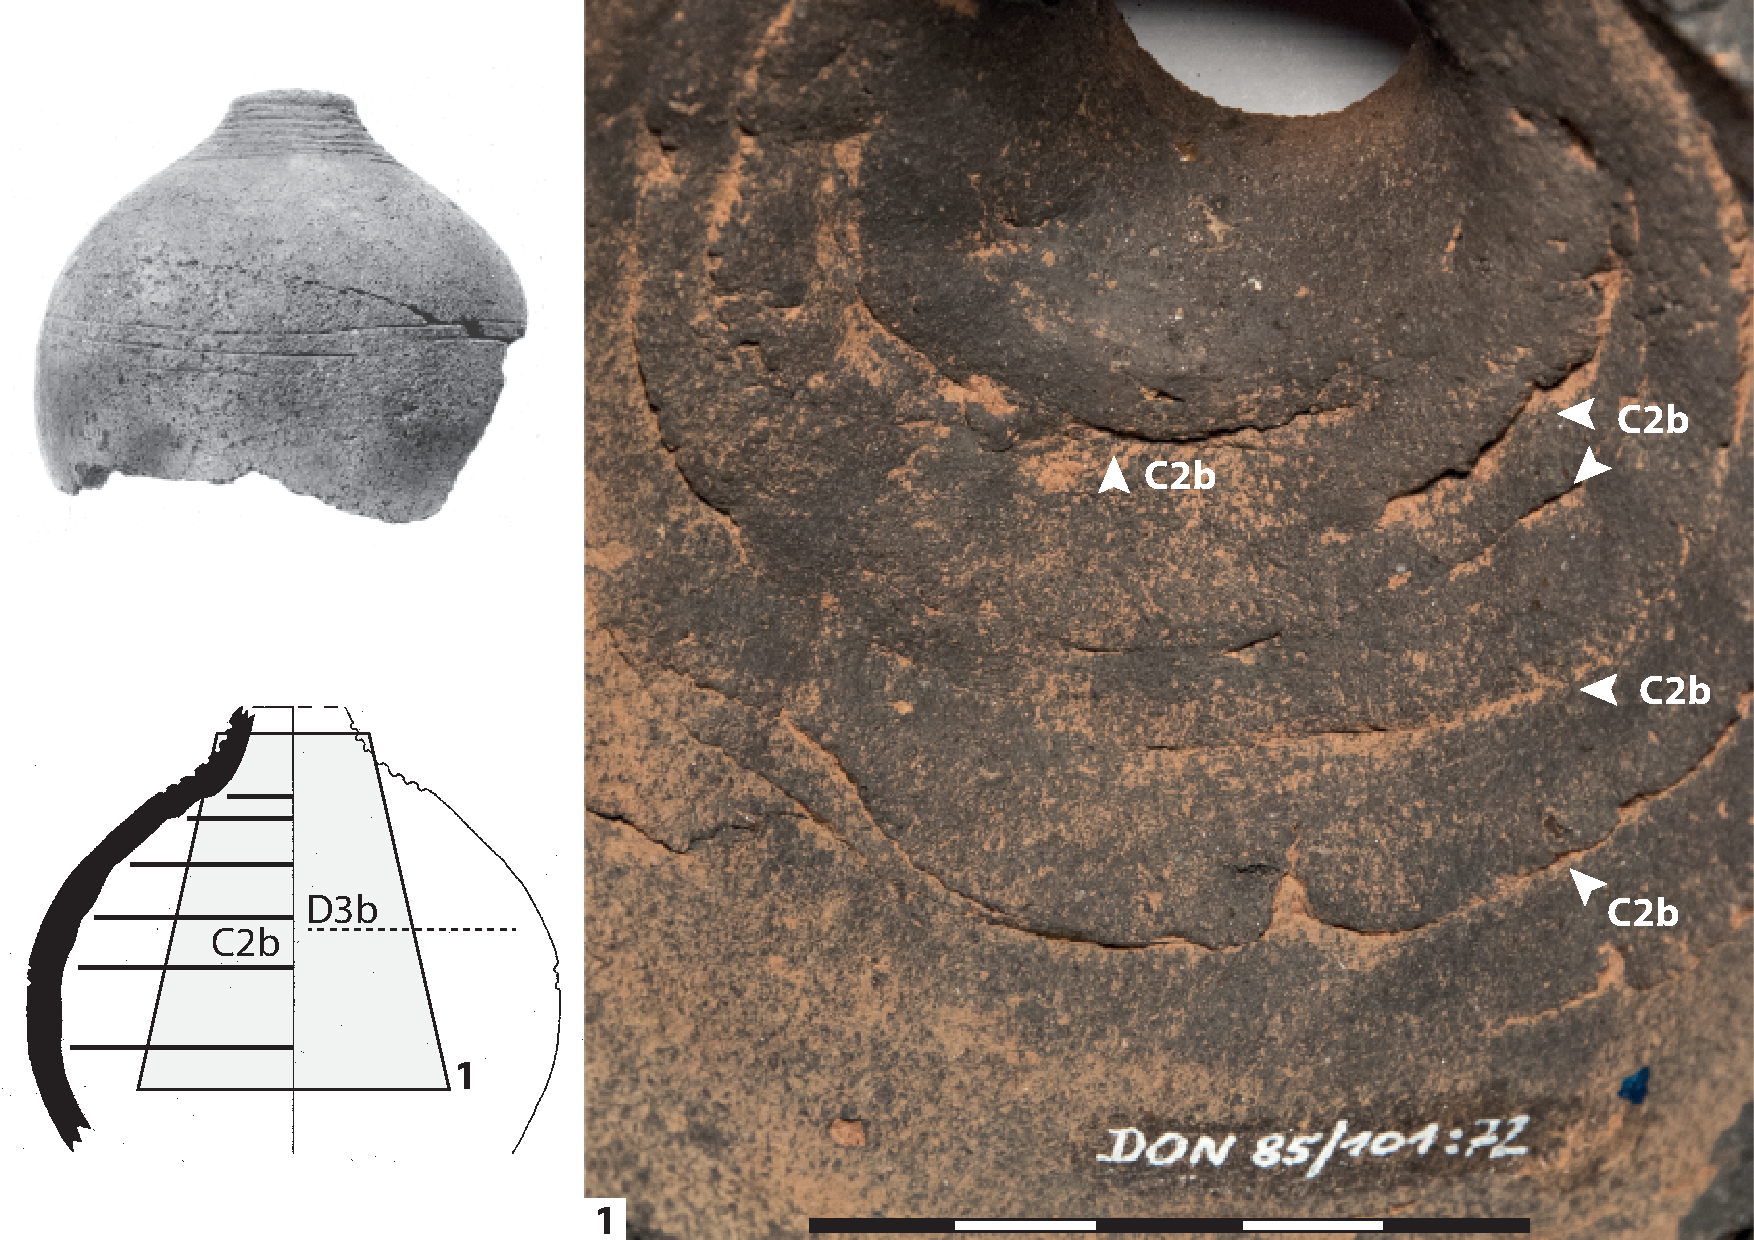
\includegraphics[height = .45\textheight]{misc/KeramikHerstellungstechnik/Gef/DON85-101-72.pdf}
		\caption{Dongo (Fpl.~202): Obj.~DON~85/101:72 (Taf.~7.14).\vspace{1em}}
		\label{DON85-101-71_Makrospuren}
	\end{subfigure}
	\begin{subfigure}{\textwidth}
		\centering
		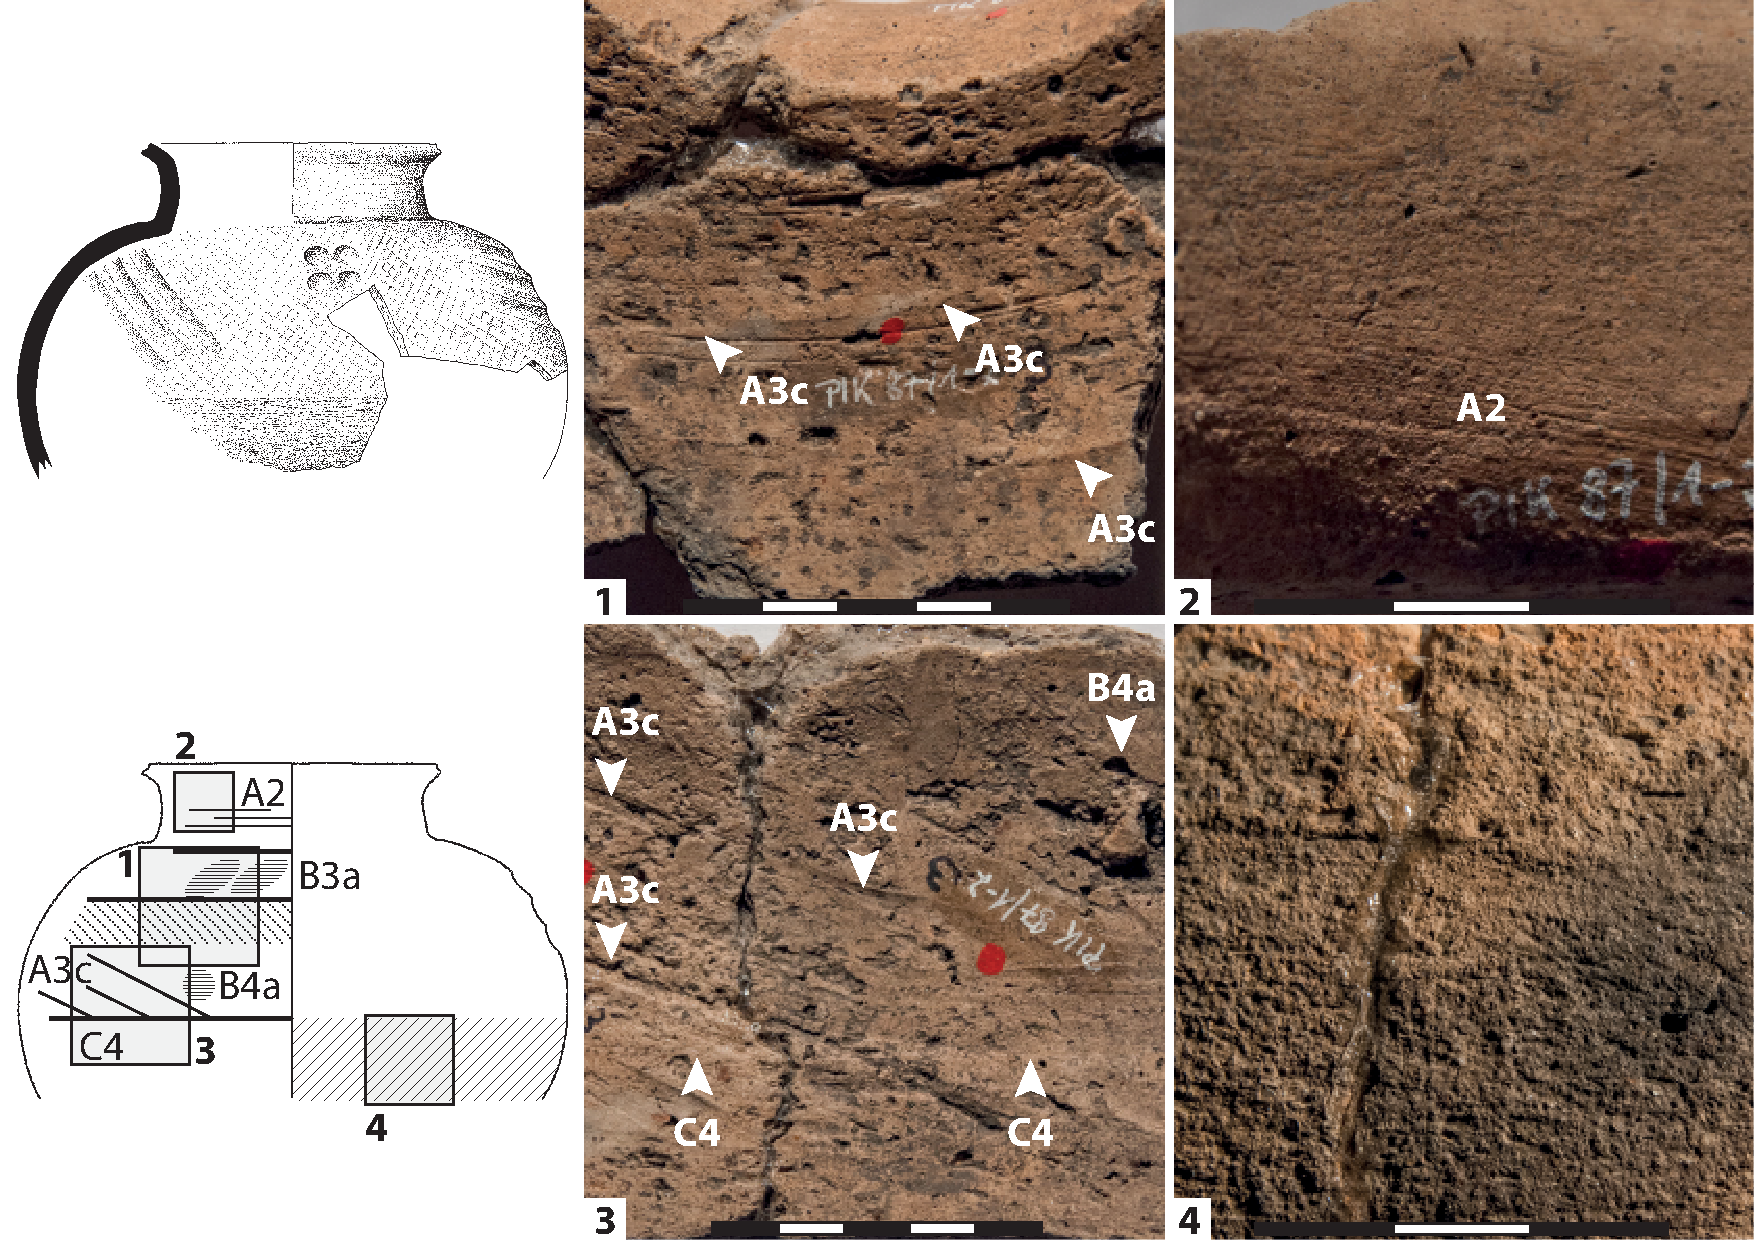
\includegraphics[height = .45\textheight]{misc/KeramikHerstellungstechnik/Gef/PIK87-1-2-3_1-3-7.pdf}
		\caption{Pikunda (Fpl.~255): Obj.~PIK~87/1-2:3 \& /1-3:7 (Taf.~47.24).}
		\label{PIK87-1-2-3_1-3-7_Makrospuren}
	\end{subfigure}
	\caption{Makrospuren: Aufnahme und Details.}
\end{figure*}

Eine aus Dongo am Ubangi stammende Flasche der gleichnamigen Stilgruppe (Kap.~\ref{sec:DON-Gr}) zeigt innen sehr deutlich nicht verstrichene Wülste (Abb.~\ref{DON85-101-71_Makrospuren}.1:~C2b). Vor allem im Bereich unterhalb des Gefäßoberteils sind die Wülste nicht überarbeitet, während sie im Bereich des Unterteils größtenteils verstrichen sind. Dies deutet an, dass das Gefäß von unten nach oben aufgebaut wurde.

Stellvertretend für das Material der Mandombe-Gruppe (Kap.~\ref{sec:MDB-Gr}) wurden zwei Gefäße aus der im Schnitt PIK~87/1 erfassten Grube A (siehe Kat.-Nr.~8) ausgewählt. Das erste Gefäß weist auf der Innenseite des fein geglätteten Halses leichte horizontale Glättspuren auf (Abb.~\ref{PIK87-1-2-3_1-3-7_Makrospuren}.2:~A2). Der innere Bereich unterhalb des Zylinderhalses ist deutlich rauer und nur grob überglättet. Unterhalb der Gefäßschulter sind horizontale, flache Grate zu beobachten sowie fingerbreite leichte Eindrücke (B3a). Letzte sind möglicherweise das Resultat einer separat erfolgten Anbringung des Halses. Deutlich unterhalb der größten Gefäßweite, in etwa auf einer Höhe mit der außen aufgebrachten Schlickerrauung, befindet sich ein markanter, horizontal verlaufender, etwa 1\,mm breiter Absatz im Profil, unterhalb derer die Wandung nach innen abrupt dicker wird (Abb.~\ref{PIK87-1-2-3_1-3-7_Makrospuren}.3:~C4). Oberhalb dieses Absatzes finden sich diagonal beziehungsweise spiralig nach oben laufende Glättrillen (A3c) sowie tiefe, bis etwa 1/3 in die Wandung ragende Eindrücke beziehungsweise Einbrüche der Gefäßwandung (Abb.~\ref{PIK87-1-2-3_1-3-7_Makrospuren}.3:~B4a). Das zweite, aus dem selben Befund stammende Gefäß weist innen ebenfalls horizontale, flache Erhöhungen beziehungsweise Grate sowie Senken auf (B3a; Taf.~47.22). Der Innenbereich des Gefäßes wurde lediglich grob überglättet, da noch viele durch ausgebrannte organische Partikel entstandene Porenräume sichtbar sind, während der Hals- und Randbereich innen -- wie auch die gesamte äußere Oberfläche -- fein geglättet und verstrichen ist. Innen, am für die Gefäße der Mandombe-Gruppe charakteristischen Zylinderhals, finden sich kurze, vertikale Risse (D3a) sowie Rillen (A2a). Der Übergang zwischen Gefäßbauch und -hals wird innen durch einen deutlichen Umbruch markiert. Es kann angenommen werden, dass der Halsbereich als separates Element aufgesetzt wurde. Beiden Stücken ist gemein, dass die Innenseite zwar grob geglättet wurde, wie die sichtbaren Glättspuren belegen (Abb.~\ref{PIK87-1-2-3_1-3-7_Makrospuren}.1, 3), die Oberfläche an allen sichtbaren Partien aber noch einmal besonders geglättet wurde. So zeigen sich im Halsbereich der Gefäße sehr feine, eng sitzende Glättspuren (siehe Abb.~\ref{PIK87-1-2-3_1-3-7_Makrospuren}.2). Diese könnten auf ein Überglätten der betreffenden Stellen mit Stoff oder Leder hindeuten; möglicherweise wurden die Bereiche auch noch einmal leicht angefeuchtet. Die nicht entsprechend behandelten Innenbereiche der Gefäße zeigen deutlich die Spuren der im Scherben vorhandenen, nunmehr ausgebrannten Organik. Eine systematische Modifikation bildet auch der Auftrag eines gröberen Schlickers auf der Gefäßunterseite (siehe Abb.~\ref{PIK87-1-2-3_1-3-7_Makrospuren}.4).

Zwei Randstücke der Konda-Gruppe (Kap.~\ref{sec:KON-Gr}), beide aus dem namensgebenden Fundplatz Konda (Fpl.~268) am oberen Sangha, zeigen innen im Schulterbereich deutliche horizontalen Lücken, die als Überreste nicht vollständig verstrichener Zwischenräume zwischen Wülsten angesprochen werden können (C2b). Für beide Stücke kann zumindest für den oberen Teil des Gefäße eine Wulstaufbautechnik postuliert werden (siehe Kap.~\ref{sec:ToepfereiEthnogr}). Da keine Bodenstücke der Konda-Gruppe bekannt sind, muss die Herstellungstechnik des Unterteils der Konda-Gefäße als unbekannt gelten.

%\addtocounter{figure}{-1}
\begin{figure*}[p]
	\centering
	\begin{subfigure}{\textwidth}
		%\setcounter{subfigure}{10}
		\centering
		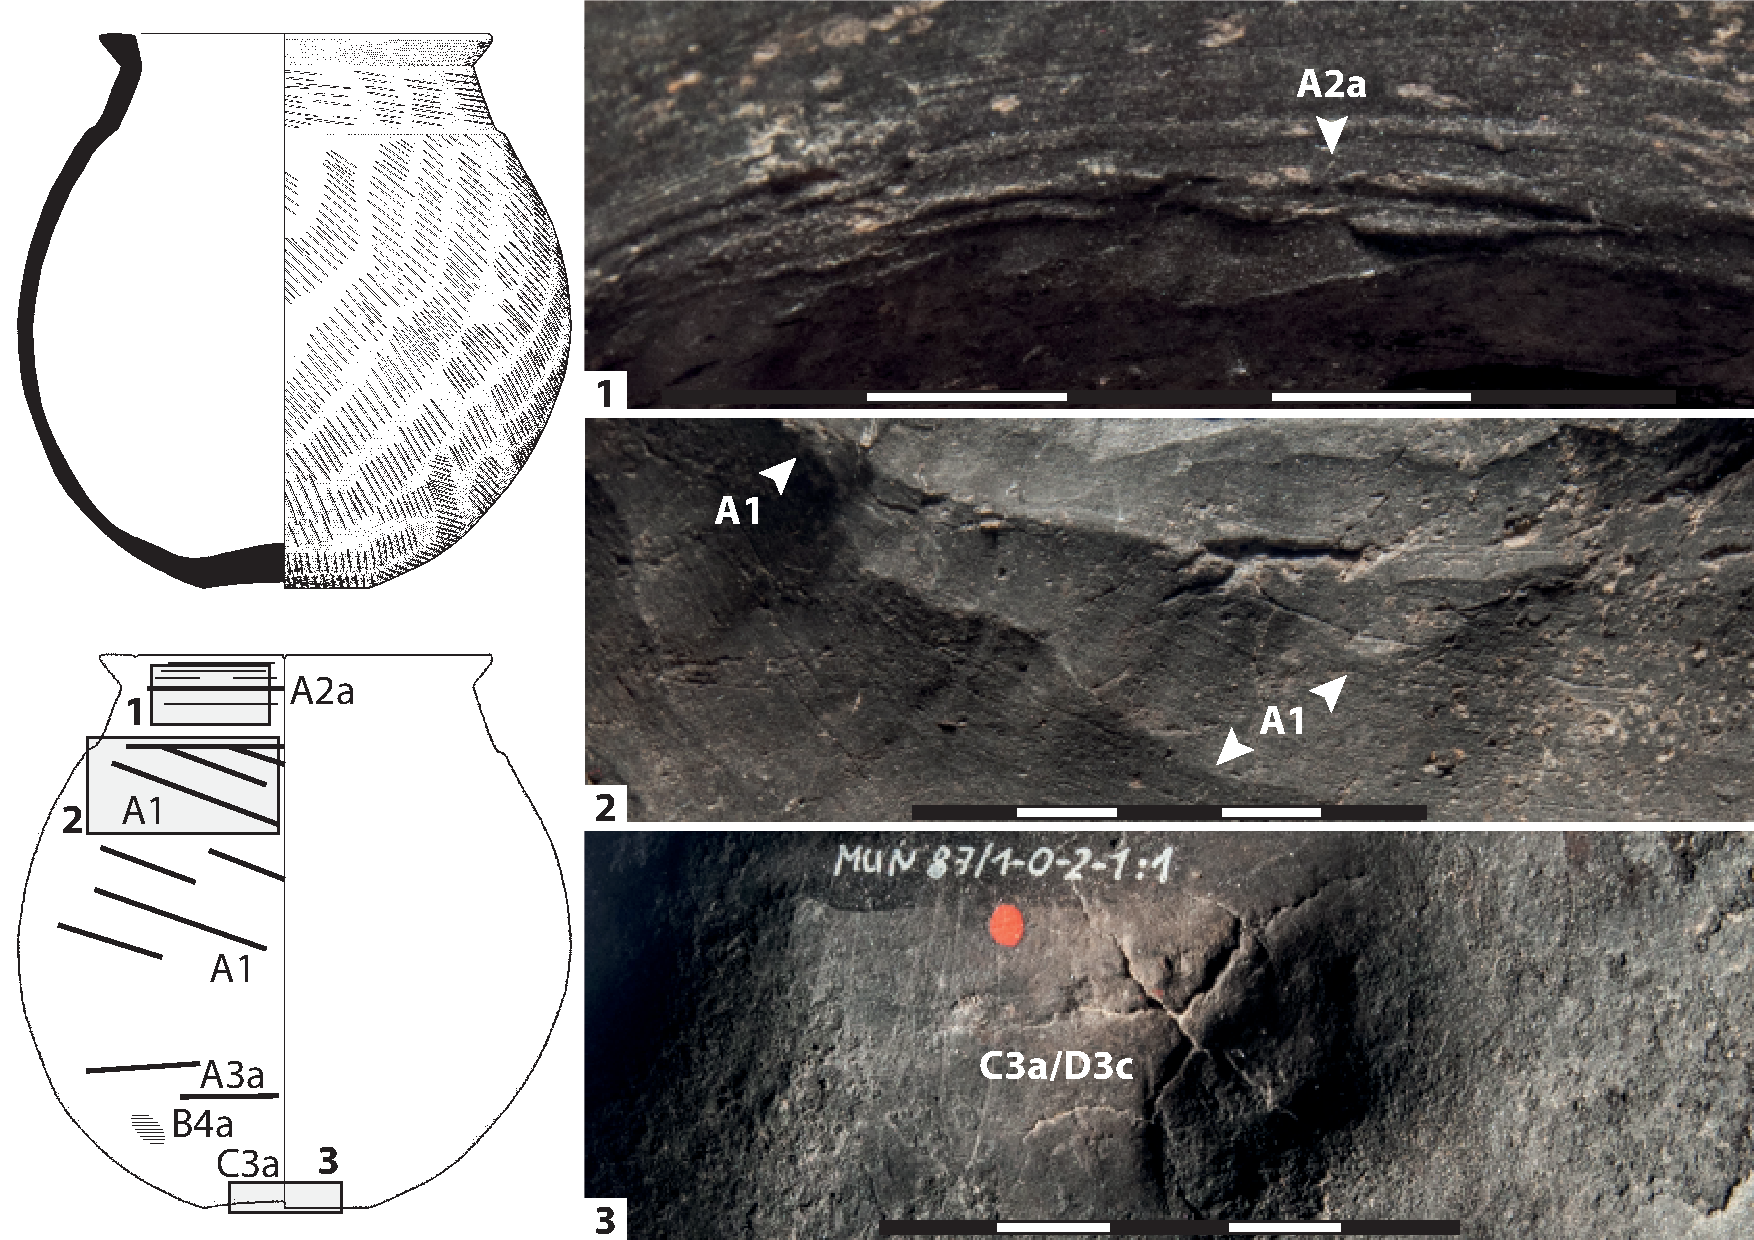
\includegraphics[height = .45\textheight]{misc/KeramikHerstellungstechnik/Gef/MUN87-1-0-2-1-1.pdf}
		\caption{Munda (Fpl.~304): Obj.~MUN~87/1-0-2-1:3 (Taf.~89.4).\vspace{1em}}
		\label{MUN87-1-0-2-1-3_Makrospuren}
	\end{subfigure}
	\begin{subfigure}{\textwidth}
		\centering
		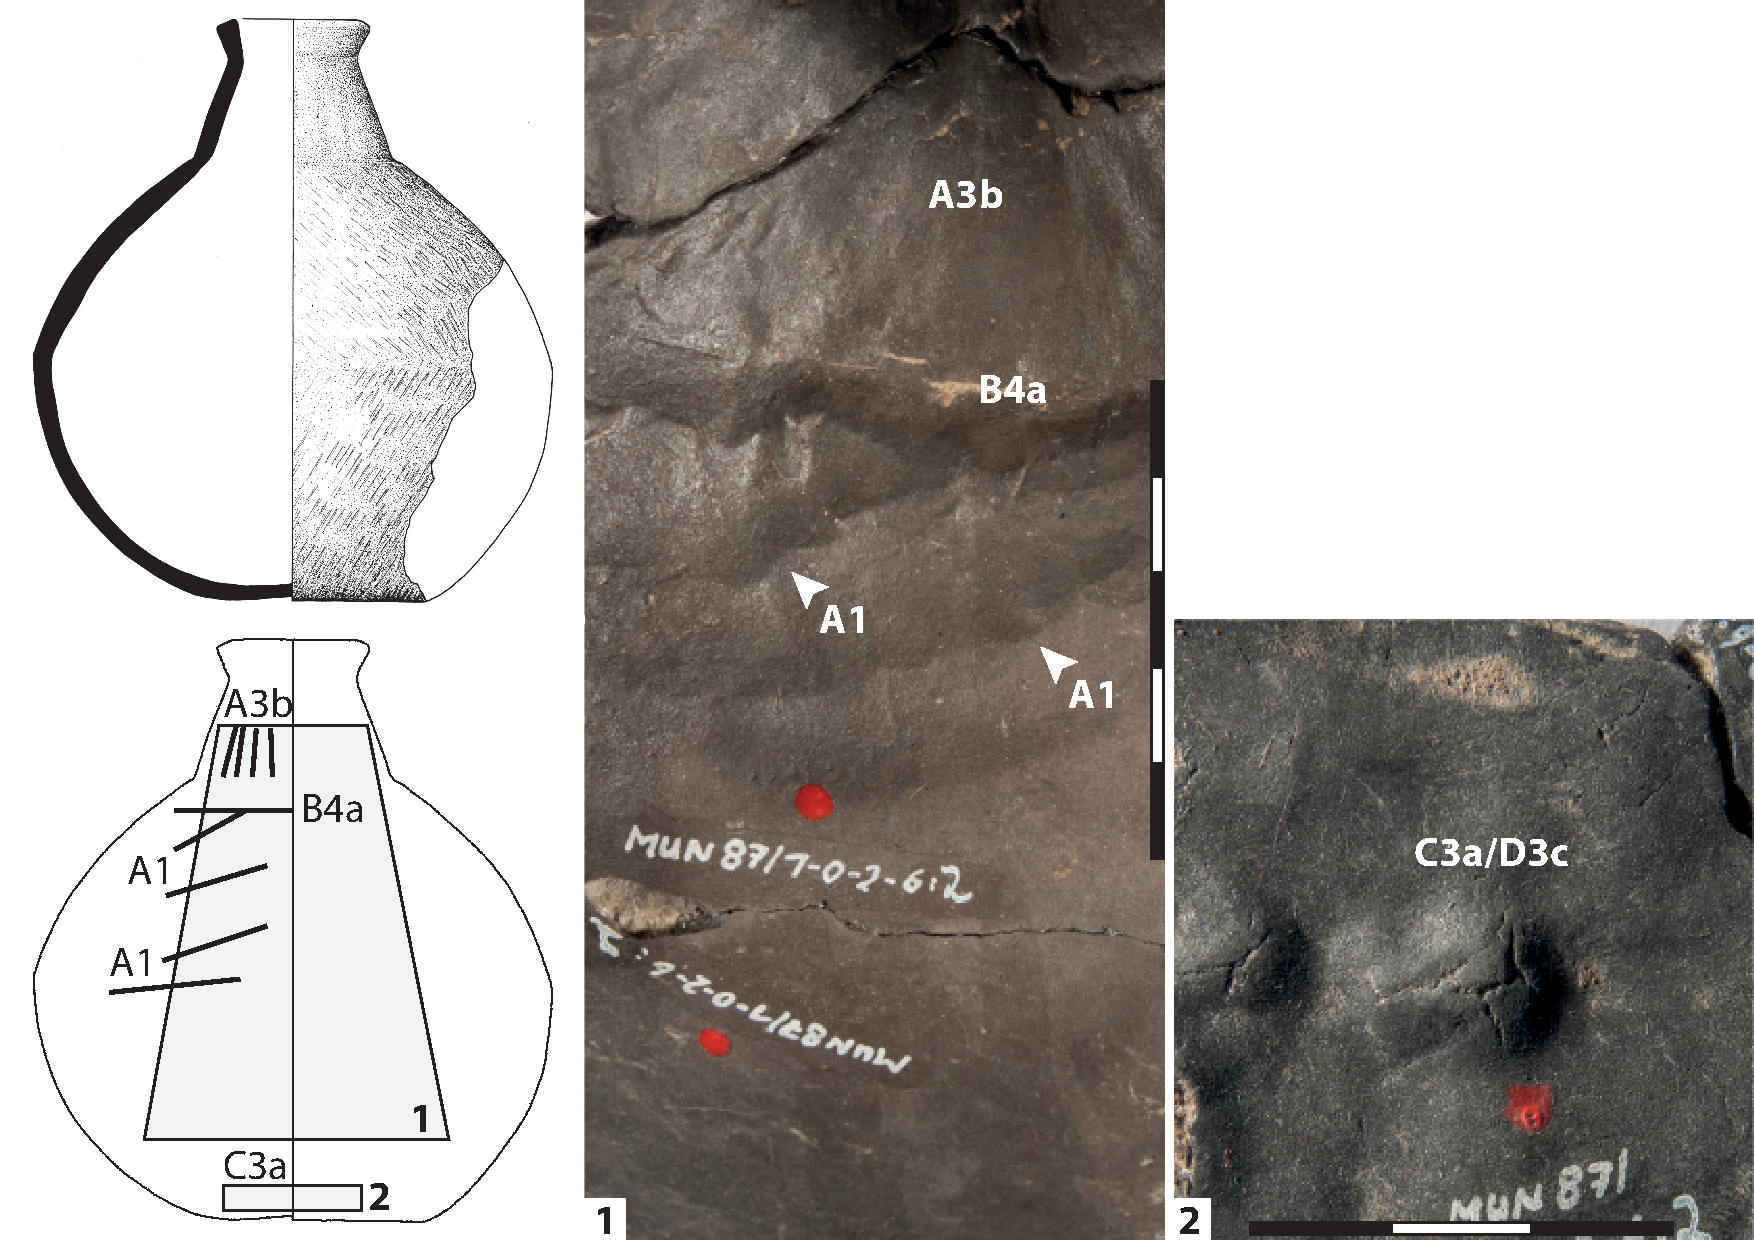
\includegraphics[height = .45\textheight]{misc/KeramikHerstellungstechnik/Gef/MUN87-1-0-2-6-2.pdf}
		\caption{Munda (Fpl.~304): Obj.~MUN~87/1-0-2-6:2 (Taf.~90.1).}
		\label{MUN87-1-0-2-6-2_Makrospuren}
	\end{subfigure}
	\caption{Makrospuren: Aufnahme und Details.}
\end{figure*}

%\addtocounter{figure}{-1}
\begin{figure*}[p]
	\centering
	\begin{subfigure}{\textwidth}
		%\setcounter{subfigure}{12}
		\centering
		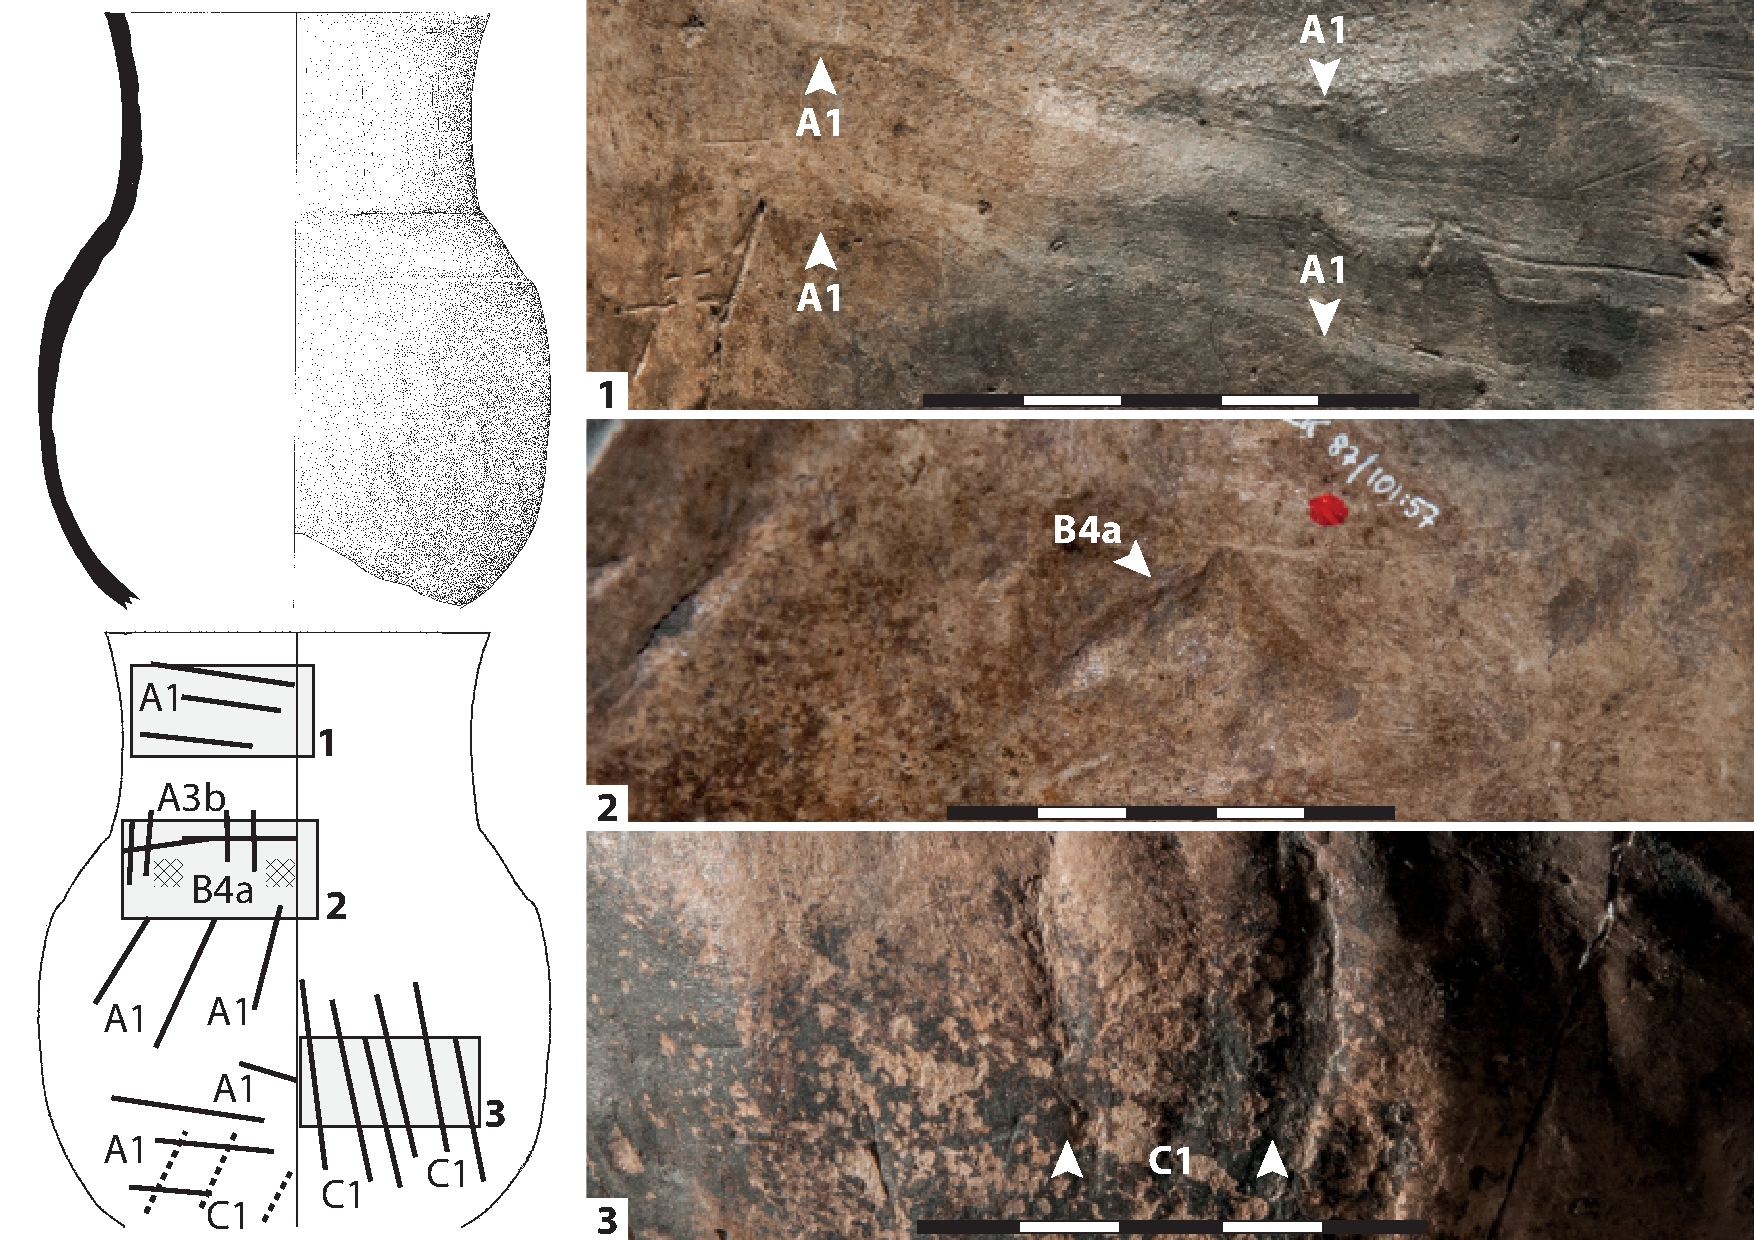
\includegraphics[height = .45\textheight]{misc/KeramikHerstellungstechnik/Gef/JEK87-101-57.pdf}
		\caption{Jeke (Fpl.~303): Obj.~JEK~87/101:57 (Taf.~88.1).\vspace{1em}}
		\label{JEK87-103-57_Makrospuren}
	\end{subfigure}
	\begin{subfigure}{\textwidth}
		\centering
		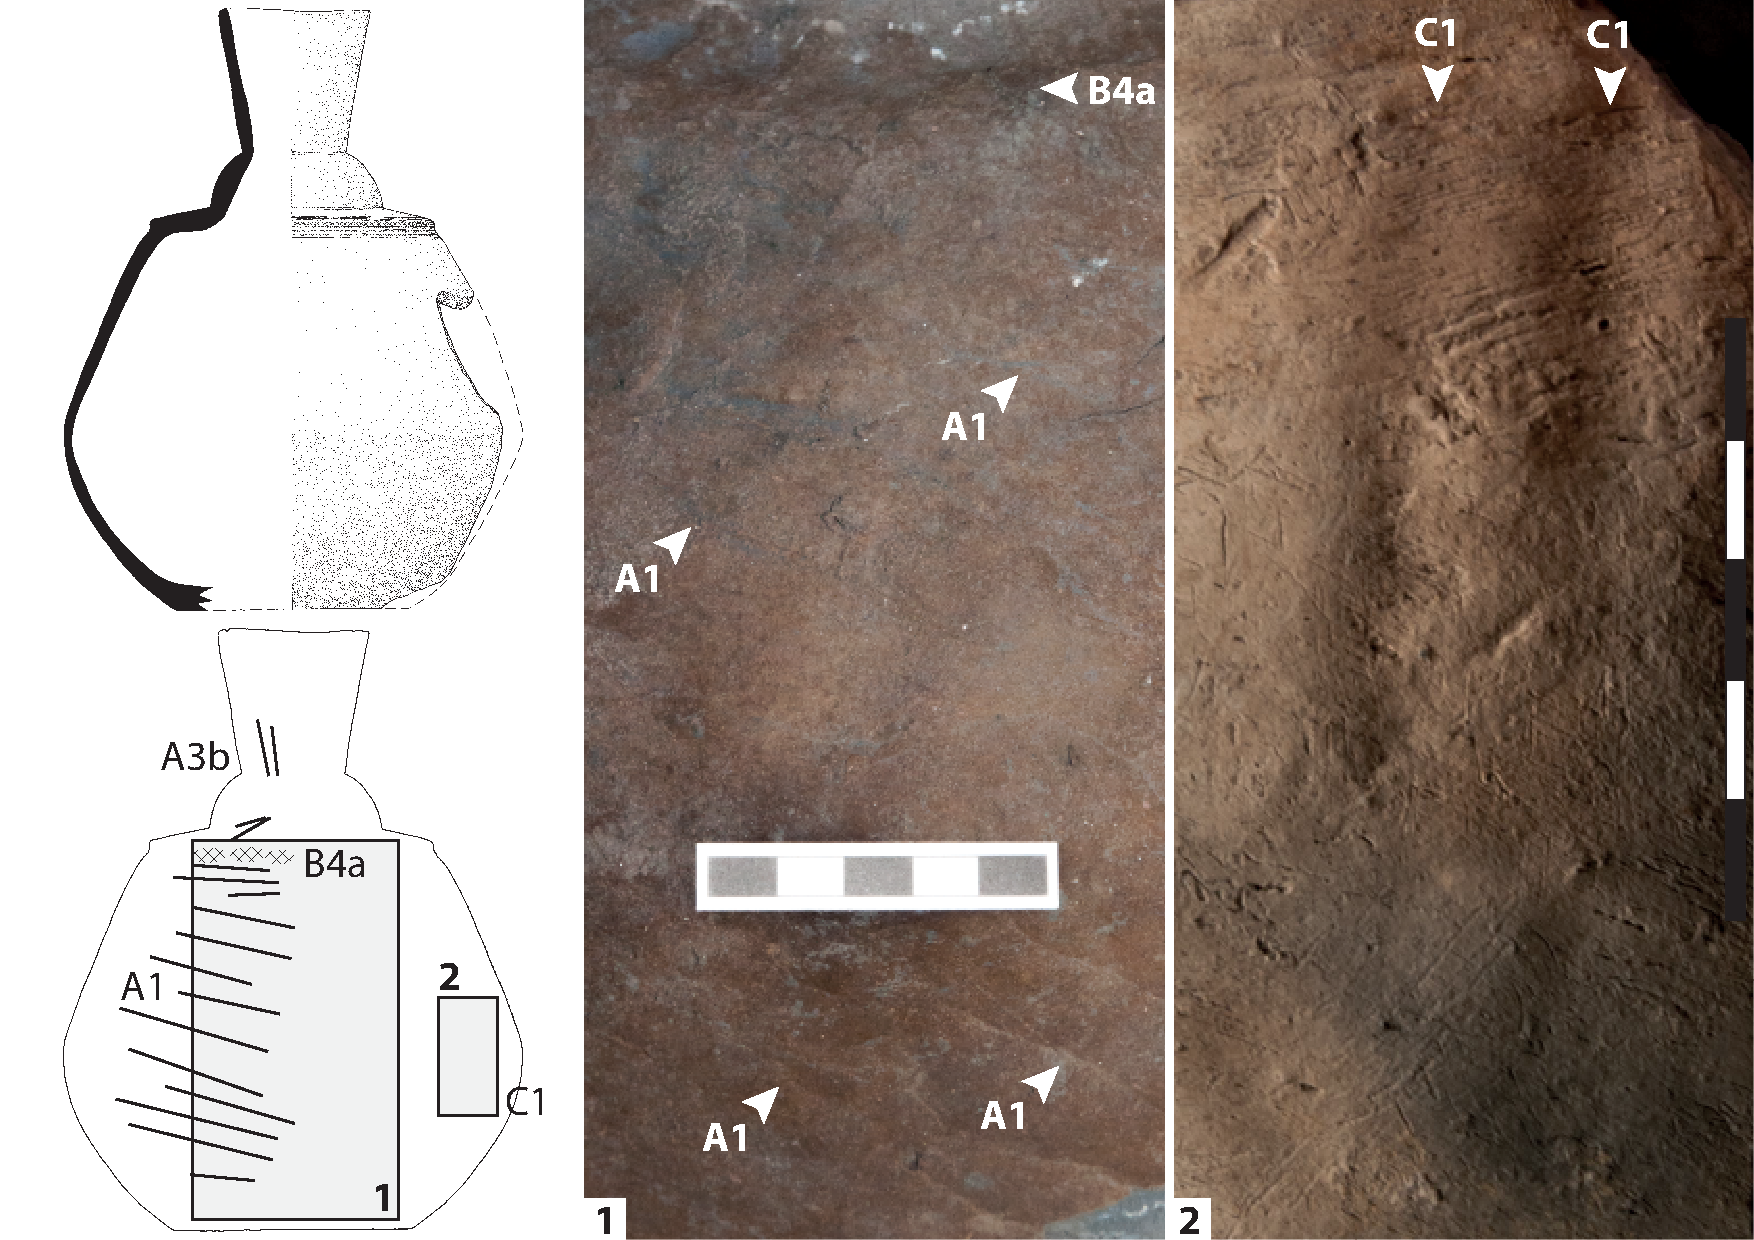
\includegraphics[height = .45\textheight]{misc/KeramikHerstellungstechnik/Gef/ITN87-103.pdf}
		\caption{Itanga (Fpl.~305): Obj.~ITN~87/103 (Taf.~97.4).}
		\label{ITN87-103_Makrospuren}
	\end{subfigure}
	\caption{Makrospuren: Aufnahme und Details.}
\end{figure*}

Die rezente Keramik des Likwala-aux-Herbes-Gebietes, die unter der Bezeichnung Epena-Gruppe (Kap.~\ref{sec:EPE-Gr}) zusammengefasst wurde, ist durch zwei Stücke vertreten. Ein Gefäß aus Jeke zeichnet sich innen durch deutliche Makrospuren aus. Im Randbereich sowie im gesamten inneren Bauchbereich zeigen sich diagonal, spiralig aufsteigende Grate (Abb.~\ref{JEK87-103-57_Makrospuren}.1:~A1). Sie weisen einen Abstand von zirka 20--30\,mm zueinander auf. Im unteren Gefäßteil beziehungsweise im Bereich des Bodenansatzes sind diese Grate von überkreuzten, ebenfalls diagonal aufsteigenden Riefen überlagert (A1). Im Schulterbereich finden sich tiefe Werkzeugspuren (Abb.~\ref{JEK87-103-57_Makrospuren}.2:~B4a), die auf das Zusammenfügen von einem separat gefertigten Hals- und Randbereich sowie dem Gefäßkörper hindeuten. Die Außenseite des Gefäßunterteils ist vertikal ziehharmonikaartig verformt (Abb.~\ref{JEK87-103-57_Makrospuren}.3:~C1). Dies kann als Hinweis gedeutet werden, dass der Boden und die Gefäßunterseite erst gegen Ende geschlossen beziehungsweise ausgeformt wurden. Eine Flasche aus Itanga zeichnet sich innen durch spiral aufsteigende Grate aus (Abb.~\ref{ITN87-103_Makrospuren}.1:~A1). Die Grate weisen einen durchgehenden Abstand von etwa 25\,mm auf und lassen eventuell auf die Glättung der Innenseite durch eine Muschel oder ein ähnliches Werkzeug schließen. Der Halsbereich wurde in einem getrennten Arbeitsschritt ausgeformt, weist innen vertikale Riefen (Abb.~\ref{ITN87-103_Makrospuren}.1:~A3b) auf, die eventuell auf eine Komprimierung des Material hindeuten, und wurde dann mit dem Gefäßkörper verbunden. Die unter der Gefäßschulter sichtbaren tiefen Eindrücke (Abb.~\ref{ITN87-103_Makrospuren}.1:~B4a) deuten auf die Nutzung eines Werkzeugs hin, um die Verbindung herzustellen. Der Boden des Gefäßes ist nicht erhalten. Die äußere Wandung ist ebenfalls, wie schon bei dem Gefäß aus Jeke, ziehharmonikaartig verformt (Abb.~\ref{ITN87-103_Makrospuren}.2:~C1), was auf eine Komprimierung von Material hindeutet.

Die Epena-Keramik lässt sich deutlich aus dem formalen Spektrum der Ebambe-Keramik ableiten (Kap.~\ref{sec:EBA-Gr}). Um den starken Bezug der beiden Stilgruppen näher zu beleuchten, wurden zwei in Munda am oberen Likwala-aux-Herbes (Fpl.~304) sowie eine aus Pikunda am mittleren Sangha (Fpl.~255) stammende GE ausgewählt.\footnote{Die Herstellung einer entsprechenden Flasche mit langem Kegelhals, die formal der Ebambe-Gruppe zugerechnet werden kann, wurde 1987 in Boleko am unteren Likwala-aux-Herbes (Fpl.~285) beobachtet (Kap.~\ref{sec:ToepfereiEthnogr}; Abb.~\ref{fig:BLK87_Töpferei}).} Eines der beiden aus Munda stammenden Gefäße weist innen markante spiralig nach oben laufende, feine Riefen beziehungsweise Grate auf (Abb.~\ref{MUN87-1-0-2-1-3_Makrospuren}.2:~A1). Unterhalb des Schulterbereiches zeigen sich weitere deutliche spiralig nach oben laufende Grate (A1). Der Übergang vom Gefäßbauch zum Halsbereich ist ebenfalls durch einen deutlichen Grat markiert. Im Hals- und Randbereich des Gefäßes sind feine Glättspuren zu beobachten (Abb.~\ref{MUN87-1-0-2-1-3_Makrospuren}.1:~A2a). Im Zentrum des leicht einziehenden Bodens befindet sich eine Verdickung, die von sternförmig verlaufenden Rissen durchzogen ist (Abb.~\ref{MUN87-1-0-2-1-3_Makrospuren}.3:~C3a, D3c). Dieses Merkmal kann als Hinweis darauf gedeutet werden, dass der Boden des Gefäßes erst zum Ende des Herstellungsprozesses geschlossen wurde, wobei in geringem Maße überschüssiges Material anfiel. Eine ebenfalls aus Munda stammende Flasche weist innen, vor allem im Schulterbereich, die gleichen, diagonal aufsteigenden flachen Grate auf (Abb.~\ref{MUN87-1-0-2-6-2_Makrospuren}.1:~A1). Der flache Boden zeichnet sich durch eine mit feinen Rissen durchzogene Verdickungen aus (Abb.~\ref{MUN87-1-0-2-6-2_Makrospuren}.2:~C3a, D3c). Dies kann darauf hindeuten, dass der Boden gegen Ende des Herstellungsprozesses geschlossen wurde. Der tiefe vertikal verlaufende Eintiefungen aufweisende Hals scheint in einem gesonderten Arbeitsprozess ausgearbeitet zu sein (Abb.~\ref{MUN87-1-0-2-6-2_Makrospuren}.1:~A3b). Sie können das Resultat einer Verengung des Material und einer damit einhergehenden Komprimierung sein. Das aus Pikunda am Sangha stammende und der Ebambe-Gruppe (Taf.~49.16) zuzurechnende Gefäßfragment zeigt im Schulterbereich feine Glättspuren (A2a) und kleine Eintiefungen (B3b). Am Gefäßbauch befinden sich diagonale bis vertikale fingerbreite Eindrücke (B3a). Die Außenseite ist im unteren Bereich des Gefäßbauches kaum geglättet und leicht rau.

%\addtocounter{figure}{-1}
\begin{figure*}[p]
	\centering
	\begin{subfigure}{\textwidth}
		%\setcounter{subfigure}{14}
		\centering
		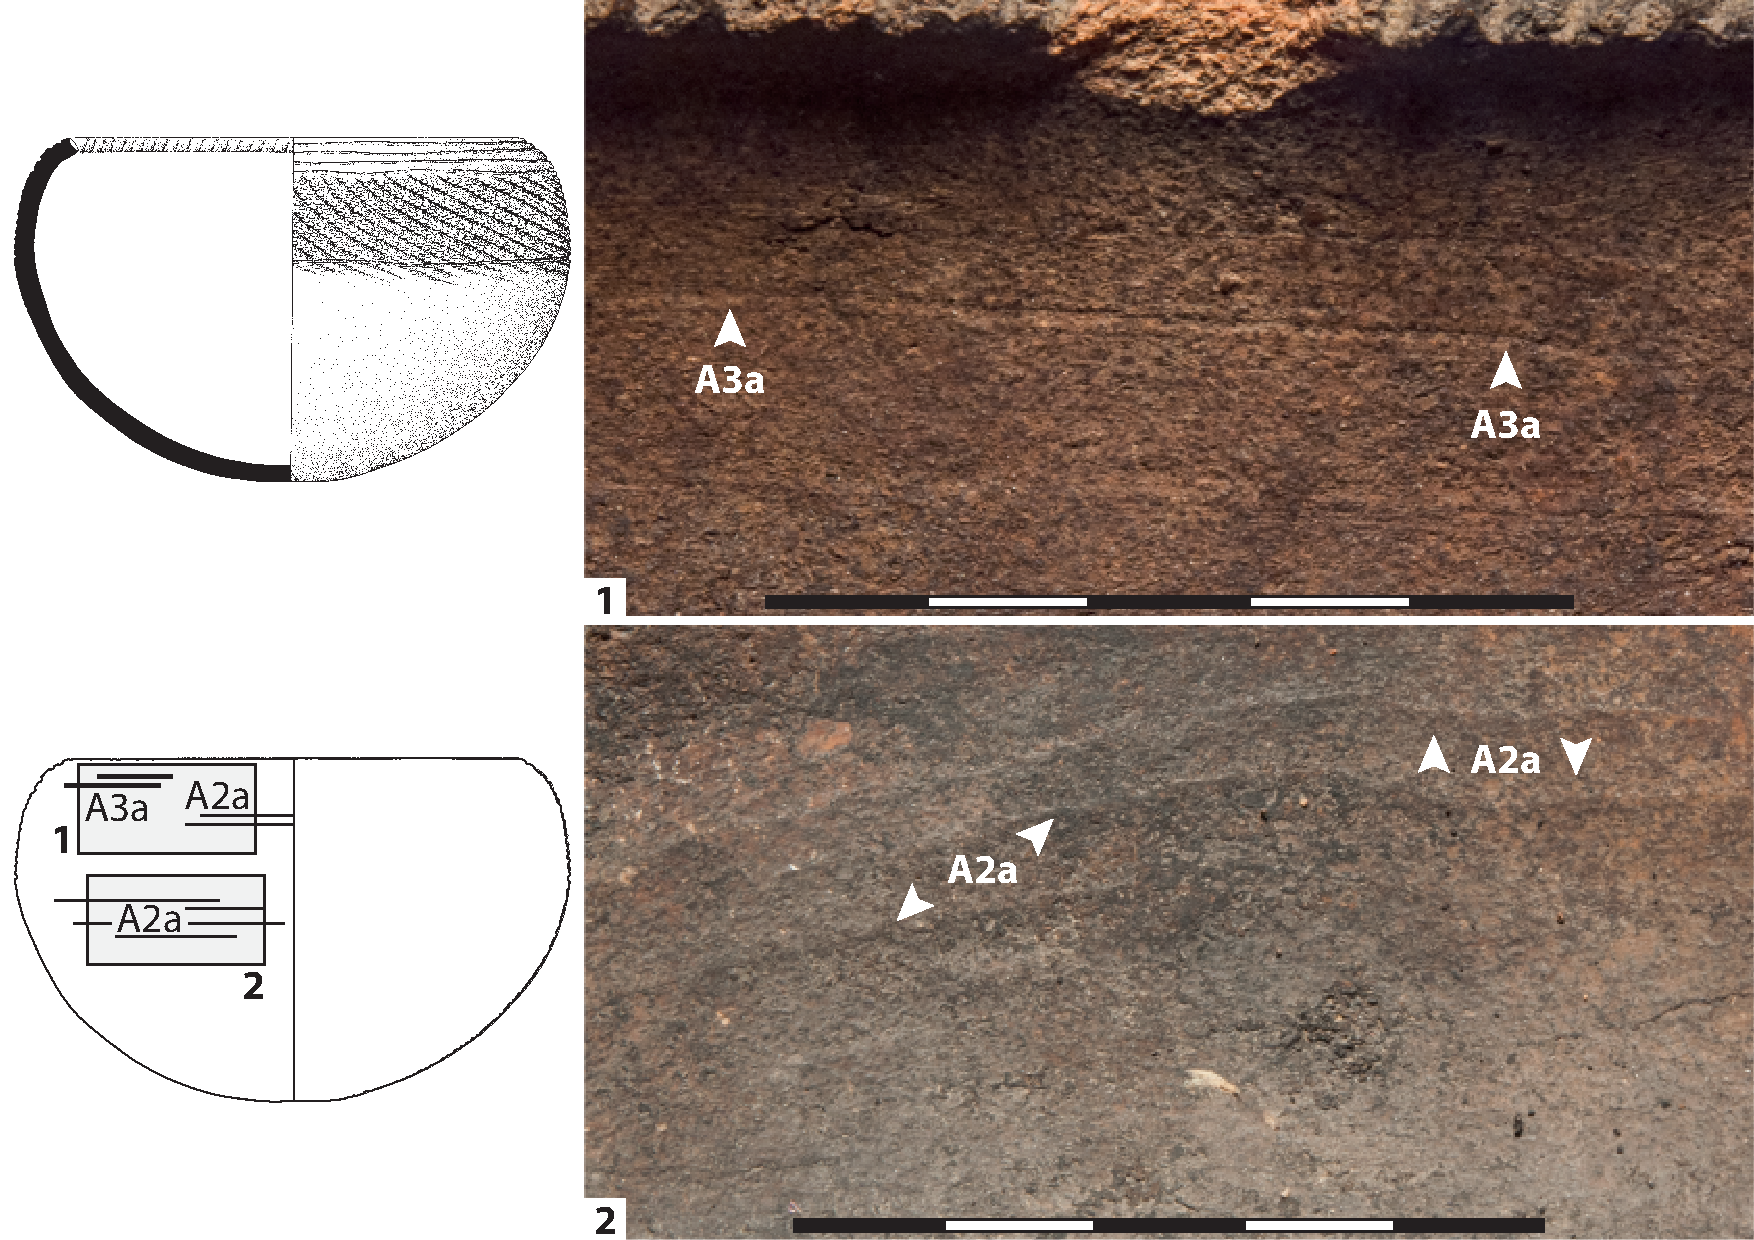
\includegraphics[height = .45\textheight]{misc/KeramikHerstellungstechnik/Gef/MBN85-501-1.pdf}
		\caption{Mbati-Ngombe (Fpl.~204): Obj.~MBN~85/501:1 (Taf.~11.1).\vspace{1em}}
		\label{MBN85-501-1_Makrospuren}
	\end{subfigure}
	\begin{subfigure}{\textwidth}
		\centering
		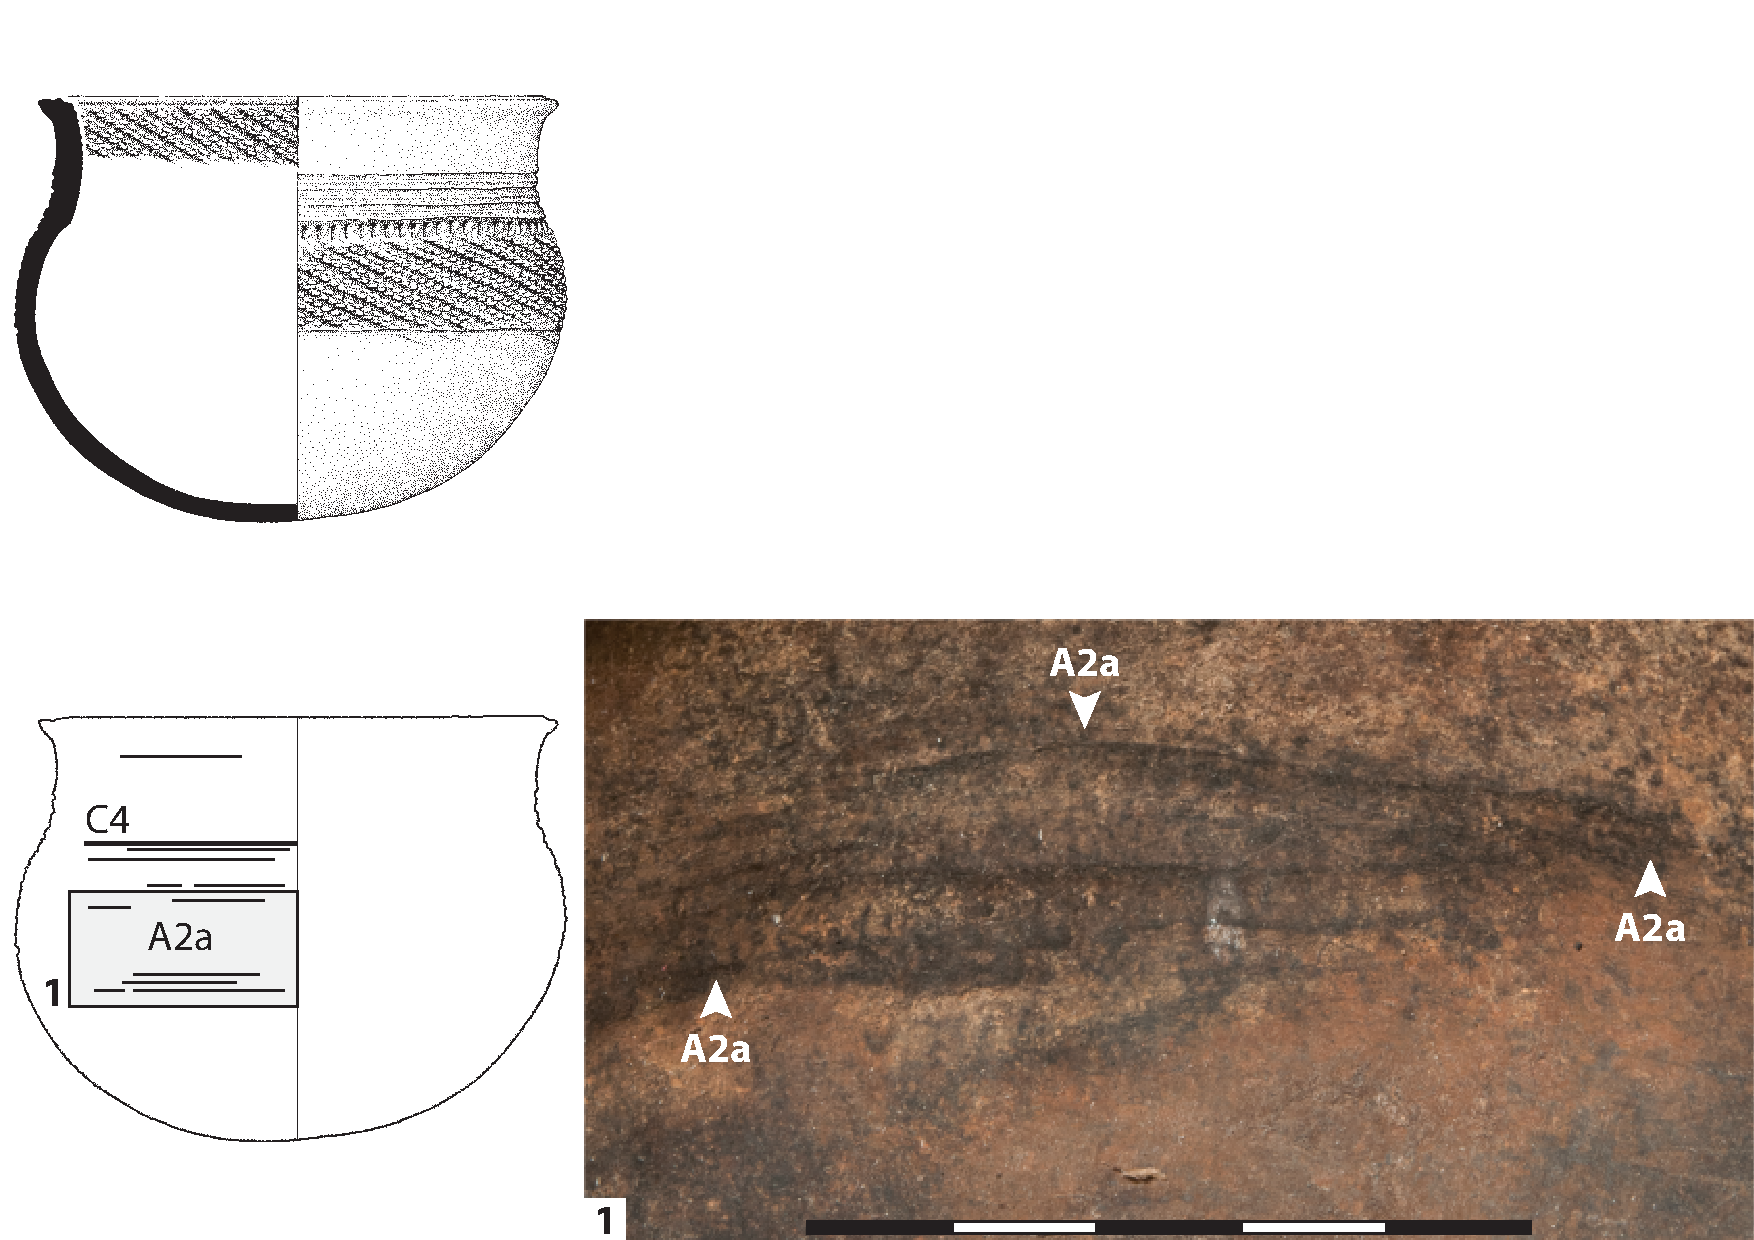
\includegraphics[height = .45\textheight]{misc/KeramikHerstellungstechnik/Gef/MBN85-501-2.pdf}
		\caption{Mbati-Ngombe (Fpl.~204): Obj.~MBN~85/501:2 (Taf.~11.2).}
		\label{MBN85-501-2_Makrospuren}
	\end{subfigure}
	\caption{Makrospuren: Aufnahme und Details.}
\end{figure*}

Die rezente Keramik entlang des mittleren Ubangi, repräsentiert durch die Mbanti-Ngombe-Gruppe (Kap.~\ref{sec:MBN-Gr}), ist durch zwei GE aus dem eponymen Fundort in der Untersuchung vertreten. Das Unterteil des ersten Gefäßes zeigt keine Makrospuren und der runde Boden weist nur leichte Unregelmäßigkeiten auf, während sich im oberen Bereich leichte, horizontale Glättspuren beobachten lassen (Abb.~\ref{MBN85-501-1_Makrospuren}.2:~A2a). Unterhalb des Randes finden sich zudem kurze, tiefere Glättriefen (Abb.~\ref{MBN85-501-1_Makrospuren}.1:~A3a). Das zweite Gefäße zeichnet sich innen auch durch feine, horizontale Glättspuren aus (Abb.~\ref{MBN85-501-2_Makrospuren}.1:~A2a). Im Bereich des Übergangs vom Bauch- zum Halsbereich zeigt sich ein deutlicher, horizontal verlaufender Grat (C4). Der Innenbereich des Gefäßbodens ist auffällig glatt und der runde Boden regelmäßig geformt.

%\addtocounter{figure}{-1}
\begin{figure*}[p]
	\centering
	\begin{subfigure}{\textwidth}
		%\setcounter{subfigure}{16}
		\centering
		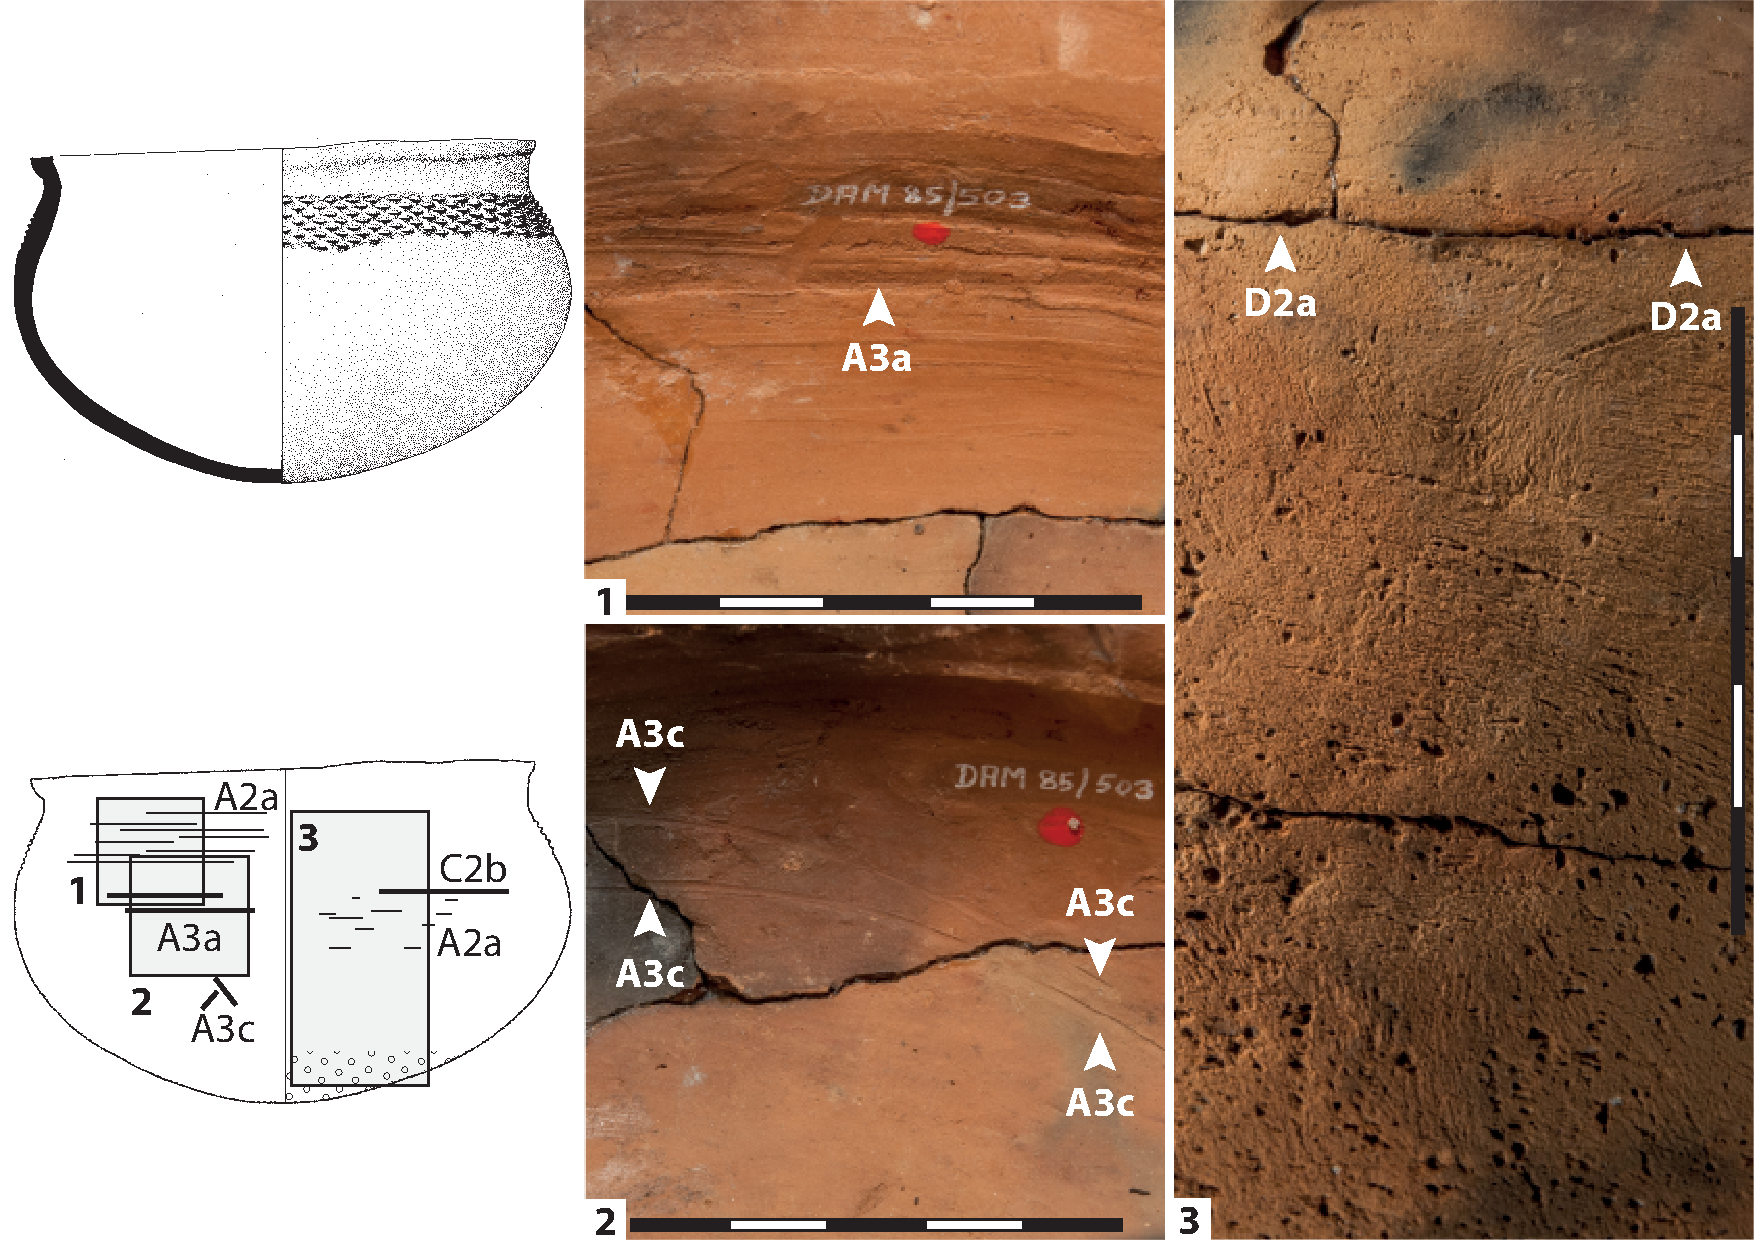
\includegraphics[height = .45\textheight]{misc/KeramikHerstellungstechnik/Gef/DAM85-503-a.pdf}
		\caption{Dama (Fpl.~222): Obj.~DAM~85/503:1 (Taf.~23.2).\vspace{1em}}
		\label{DAM85-503-1_Makrospuren}
	\end{subfigure}
	\begin{subfigure}{\textwidth}
		\centering
		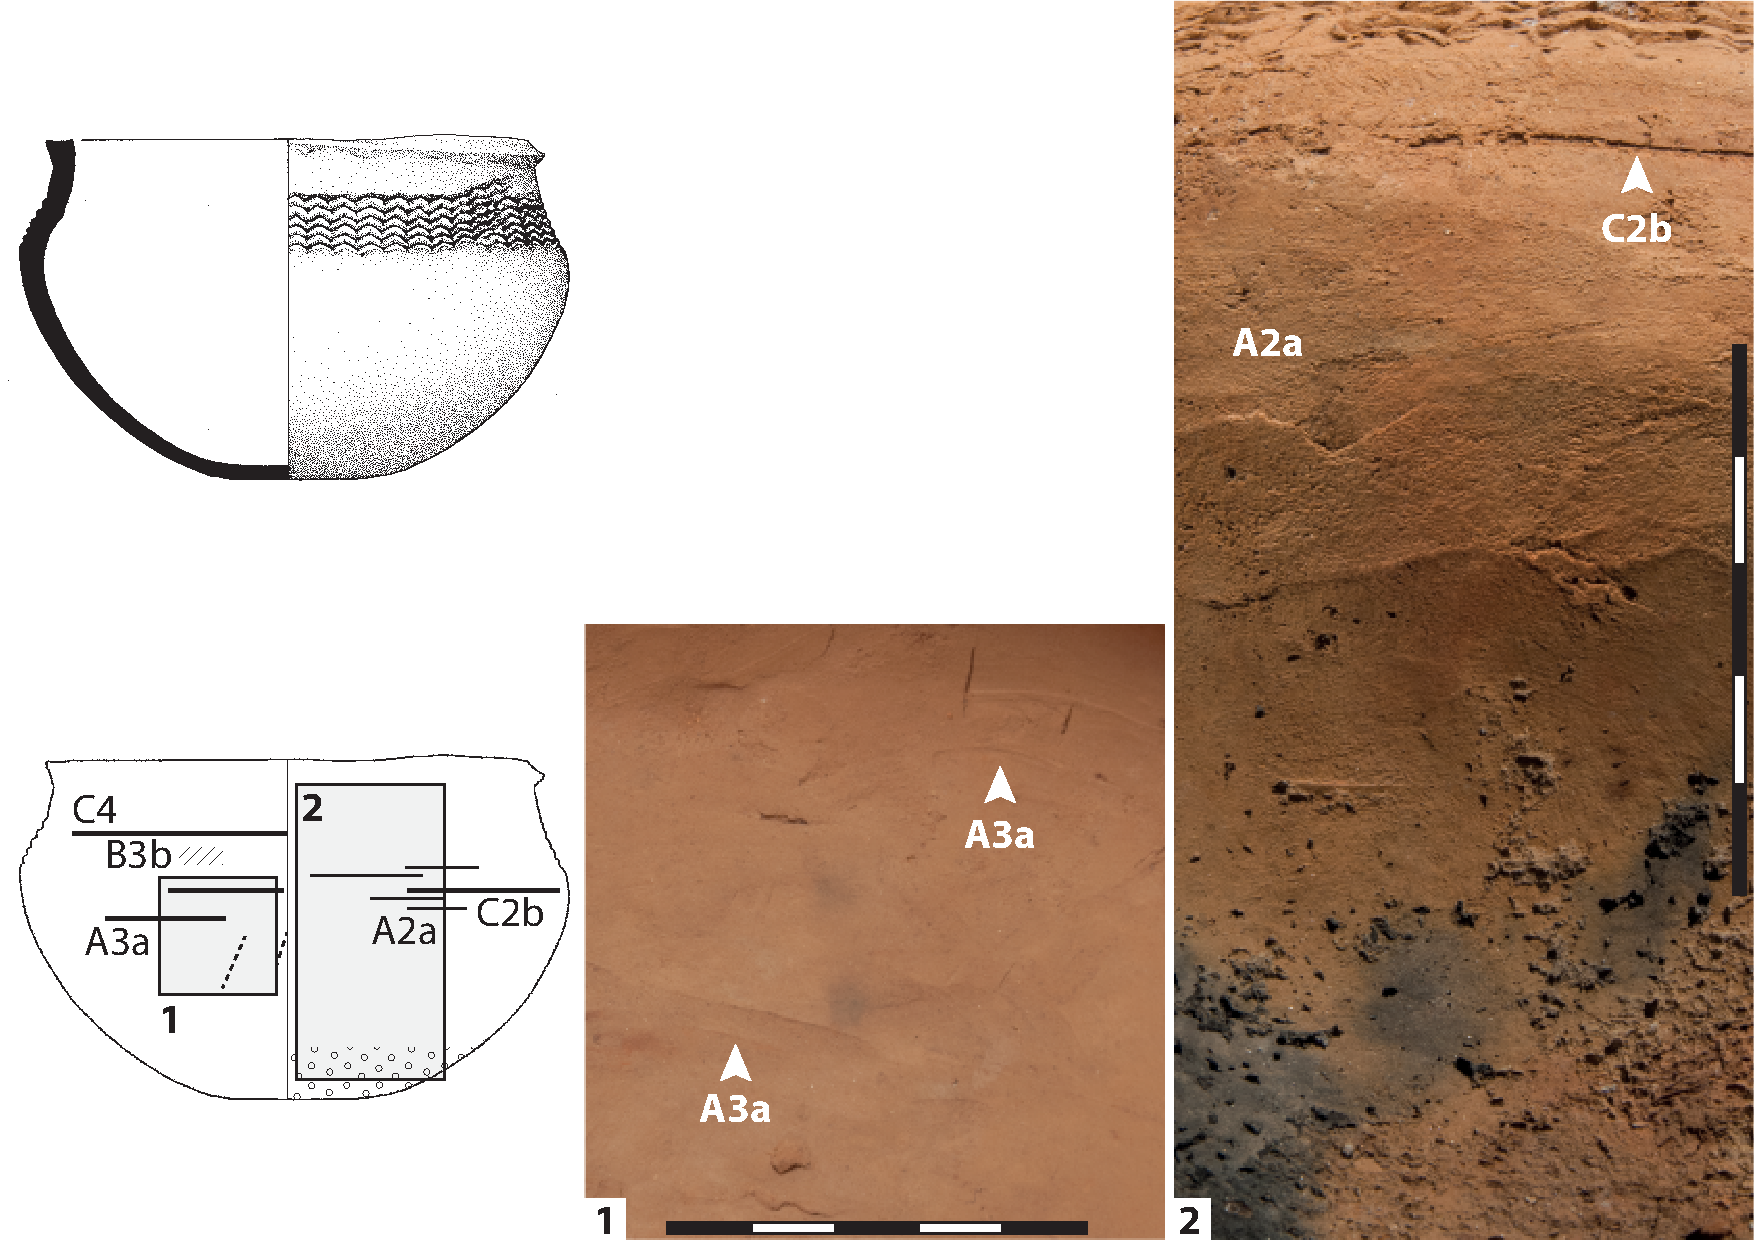
\includegraphics[height = .45\textheight]{misc/KeramikHerstellungstechnik/Gef/DAM85-503-b.pdf}
		\caption{Dama (Fpl.~222): Obj.~DAM~85/503:2 (Taf.~23.3).}
		\label{DAM85-503-2_Makrospuren}
	\end{subfigure}
	\caption{Makrospuren: Aufnahme und Details.}
\end{figure*}

Die weiter nördlich, entlang des mittleren bis oberen Ubangi verbreitete, rezente Dama-Gruppe (Kap.~\ref{sec:DAM-Gr}) wird durch zwei Gefäße repräsentiert, deren Herstellung 1985 im eponymen Fundort direkt beobachtet werden konnte (Kap.~\ref{sec:DAM_Herstellung}). Das erste Gefäß ist beim späteren Brand durch das \textit{River Reconnaissance Project} zersprungen. Auffällig sind die vornehmlich horizontalen Brüche (Abb.~\ref{DAM85-503-1_Makrospuren}.3:~D2a) knapp oberhalb des größten Durchmessers, die auf den Aufbau in zwei Abschnitten hinweisen. Außen finden sich lediglich im Bereich knapp unterhalb der größten Gefäßweite einige feine und kurze Glättspuren (A2a). Der kurz ausgeformte Halsbereich weist innen horizontale, eng sitzende, feine Glättriefen auf (A2a). Im Bereich der größten Gefäßweiten finden sich zirka 5--10\,cm lange, zwar deutlich bogenförmige aber grundsätzlich horizontal ausgerichtete, tiefe Riefen (Abb.~\ref{DAM85-503-1_Makrospuren}.1:~A3a). Unterhalb der größten Weite lassen sich lediglich kurze, diagonal verlaufende und sich stellenweise überlagernde, feine Riefen beobachten (Abb.~\ref{DAM85-503-1_Makrospuren}.2:~A3c). Das Gefäßunterteil ist sehr regelmäßig ausgeformt.	Das zweite, intakt gebliebene Gefäß zeigt auf der Außenseite im Bereich des größten Durchmessers feine horizontale, leicht bogenförmige Glättspuren (Abb.~\ref{DAM85-503-2_Makrospuren}.2:~A2a). Knapp oberhalb des größten Durchmessers ist ein horizontal verlaufender, teilweise überstrichener Grad (Abb.~\ref{DAM85-503-2_Makrospuren}.2:~C2b), der die Grenze zwischen zwei unterschiedlich gefertigten Gefäßteilen markiert. Innen ist der Ansatz des Halses durch einen deutlichen Grad markiert (C4). Im Bereich des Gefäßbauches finden sich bogenförmige tiefe Glättspuren (Abb.~\ref{DAM85-503-2_Makrospuren}.1:~A3a) sowie feine, diagonale wirbelähnliche Aufhäufungen von Ton. Im Schulterbereich sind auf der Innenseite einige Eintiefungen (B3b) zu beobachten. Der Gefäßboden ist sehr symmetrisch und gleichmäßig ausgearbeitet. Beide Gefäße zeigen Abplatzungen der äußeren Oberfläche im Bereich der Gefäßböden. Diese wurden als nicht beabsichtigt angesehen und in den weiteren Betrachtungen ausgelassen. Inwieweit sie darauf zurück zu führen sind, dass die Gefäße in einer kleinen Erdgrube gefertigt wurden (Kap.~\ref{sec:ToepfereiEthnogr}) und keine konkav geformte \enquote*{Schablone}, wie ein altes Gefäßfragment, genutzt wurde, muss im Rahmen dieser Betrachtungen offen bleiben.

\vspace{1.5em}
\noindent Basierend auf den beobachteten Makrospuren der untersuchten Gefäße ließen sich diese in drei Gruppen gliedern (Tab.~\ref{tab:Makrospuren_ChaineOperatoire}). Die Gruppe A bilden Gefäße, die grundsätzlich in einem Arbeitsgang, von unten nach oben aufgebaut wurden und horizontal orientierte Schwankungen der Wandungsdicke (C2a) oder sogar sichtbare, unverstrichene Wülste aufweisen (siehe Abb.~\ref{DON85-101-71_Makrospuren}.1). Weitere Indizien, die für die Zuweisung zu dieser Gruppe herangezogen wurden, sind ein diagonal verlaufender, interner Aufbau der Bruchflächen gemäß \textcite[140 Abb.~8.b]{Lindahl.2010} sowie vornehmlich horizontale, durch den Gefäßkörper laufende Bruchlinien (D2a) oder Risse (D3a). Gruppe B zeichnet sich vornehmlich durch Hinweise darauf aus, dass der Aufbau vom Rand zum Boden hin und in zwei Teilen erfolgte. Beobachtungen, wonach der Boden mutmaßlich erst zum Ende des Arbeitsprozesses geschlossen oder ausgeformt wurde, lassen sich aus Verengungen des Gefäßdurchmessers und damit einhergehenden vertikal laufenden ziehharmonikaartigen \enquote*{Rippen} (C1), die sich vor allem oberhalb des Bodenansatzes finden, ableiten. Ebenfalls können buckelartige, isolierte Verdickungen der Gefäßboden (C3a) oder eine drastische Ausdünnung des Boden (C3b) als Indizien dafür gewertet werden, dass der Boden ausschließlich mit vorhandenem Material geschlossen oder ausgeformt wurde. Die beobachteten buckelartigen Verdickungen des Gefäßbodens zeigen häufig auch radiale laufende beziehungsweise sternförmige Risse, die ebenfalls andeuten, dass der Boden nicht aus einem Stück gefertigt wurde (siebe Abb.~\ref{MUN87-1-0-2-1-3_Makrospuren}--b). Des Weiteren lässt sich bei Gefäßen der Gruppe B ein lagiger Aufbau der in den Bruchflächen sichtbaren, inneren Struktur des Scherbens ausmachen (ebd. 140 Abb.~8.c--d). Zudem können vornehmlich diagonal durch den Gefäßkörper laufende Brüche (D2b) sowie Risse (D3b) als Indikatoren für die Zuweisung zu Gruppe B gelten. Die Gefäße der Gruppe C zeichnen sich durch äußerst regelmäßig geformte, runde Boden beziehungsweise Gefäßunterteile aus. Die Unterteile haben häufig einen stark komprimierten und dichten Scherben. Oft sind die Gefäße dieser Gruppe in zwei Teilen hergestellt, mit einem deutlich sicht- oder fühlbaren Übergang. 


\section{Traditionelle Töpferei und ethnoarchäologischer Vergleich}\label{sec:ToepfereiEthnogr}

Im Zuge der Untersuchung der beobachtbaren Makrospuren, die Hinweise auf die Herstellungstechniken der Gefäße geben, wurde eine stichprobenhafte Recherche rezenter Töpfereibelege unternommen. Die umfangreiche ethnografische Studie von \textcite[44]{Drost.1967} unterscheidet drei grundsätzliche Grundtechniken: Treiben, Abformen und Aufbauen. Beim Treiben wird der Gefäßkörper durch Herausdrücken aus einem Klumpen, aus dem Vollen hergestellt, während das Abformen auf der Nutzung einer konkaven oder konvexen Vorlage basiert. Die dritte Grundtechnik, das Aufbauen, basiert auf dem Zusammenfügen einzelner Teile, vornehmlich einzelner Wülste. Zusätzlich zu den ethnografisch beschriebenen Beispielen für rezente Töpfereitechniken wurden die Töpfereitraditionen des Arbeitsgebietes, wie auch des Inneren Kongobeckens, im Rahmen der Prospektionen des \textit{River Reconnaissance Project} direkt beobachtet und dokumentiert. Eine dezidierte Auswertung der im Zusammenhang mit diesen ethnografischen Beobachtungen gemachten Interviews und Beschreibungen liegt zum gegenwärtigen Zeitpunkt nicht vor.\footnote{Eine umfangreiche Veröffentlichung der im Zuge des \textit{River Reconnaissance Project} dokumentierten Belege rezenter Töpfereitechnologien, mit besonderem Fokus auf die Töpferei aus Ikenge am Ruki, ist gegenwärtig in Vorbereitung \parencite{Eggert.inVorb.}.} Die jeweilige fotografische Dokumentation hingegen kann hier in Auszügen wiedergegeben werden. 

\begin{figure*}[p]
	\centering
	\begin{subfigure}[t]{0.32\textwidth}
		\centering
		\includegraphics[width = \textwidth]{figs/MBN85_E85-017-32.jpg}
		\caption{Werkzeuge.}
		\label{fig:MBN85_Töpferei_a}
	\end{subfigure}
	\begin{subfigure}[t]{0.32\textwidth}
		\centering
		\includegraphics[width = \textwidth]{figs/MBN85_E85-018-06.jpg}
		\caption{Wulstaufbau.}
		\label{fig:MBN85_Töpferei_b}
	\end{subfigure}
	\begin{subfigure}[t]{0.32\textwidth}
		\centering
		\includegraphics[width = \textwidth]{figs/MBN85_E85-018-09.jpg}
		\caption{Tonring und Rohling.}
		\label{fig:MBN85_Töpferei_d}
	\end{subfigure}
	\begin{subfigure}[t]{0.32\textwidth}
		\centering
		\includegraphics[width = \textwidth]{figs/MBN85_E85-018-12.jpg}
		\caption{Weiterer Wulstaufbau.}
		\label{fig:MBN85_Töpferei_c}
	\end{subfigure}
	\begin{subfigure}[t]{0.32\textwidth}
		\centering
		\includegraphics[width = \textwidth]{figs/MBN85_E85-018-13.jpg}
		\caption{Rohling auf Tonring.}
		\label{fig:MBN85_Töpferei_e}
	\end{subfigure}
	\begin{subfigure}[t]{0.32\textwidth}
		\centering
		\includegraphics[width = \textwidth]{figs/MBN85_E85-018-25.jpg}
		\caption{Zwei Rohlinge.}
		\label{fig:MBN85_Töpferei_f}
	\end{subfigure}
	\begin{subfigure}[t]{0.32\textwidth}
		\centering
		\includegraphics[width = \textwidth]{figs/MBN85_E85-018-32.jpg}
		\caption{Glätten der Wandung.}
		\label{fig:MBN85_Töpferei_g}
	\end{subfigure}
	\begin{subfigure}[t]{0.32\textwidth}
		\centering
		\includegraphics[width = \textwidth]{figs/MBN85_E85-018-35.jpg}
		\caption{Überblick.}
		\label{fig:MBN85_Töpferei_h}
	\end{subfigure}
	\begin{subfigure}[t]{0.32\textwidth}
		\centering
		\includegraphics[width = \textwidth]{figs/MBN85_E85-018-36.jpg}
		\caption{Abschneiden des Randes.}
		\label{fig:MBN85_Töpferei_i}
	\end{subfigure}
	\begin{subfigure}[t]{0.32\textwidth}
		\centering
		\includegraphics[width = \textwidth]{figs/MBN85_E85-019-9.jpg}
		\caption{Glätten.}
		\label{fig:MBN85_Töpferei_j}
	\end{subfigure}
	\begin{subfigure}[t]{0.32\textwidth}
		\centering
		\includegraphics[width = \textwidth]{figs/MBN85_E85-019-18.jpg}
		\caption{Verzierung.}
		\label{fig:MBN85_Töpferei_k}
	\end{subfigure}
	\begin{subfigure}[t]{0.32\textwidth}
		\centering
		\includegraphics[width = \textwidth]{figs/MBN85_E85-019-26.jpg}
		\caption{Vegetabilische Roulette.}
		\label{fig:MBN85_Töpferei_l}
	\end{subfigure}
	\caption{Mbati Ngombe (Fpl.~204): Herstellung von Keramikgefäßen\\(Fotos: M.~K.~H. Eggert).}
	\label{fig:MBN85_Töpferei}
\end{figure*}

\subsection*{Mbati-Ngombe (Fpl.~204)}\label{sec:MBN_Herstellung}

Im Zuge der Prospektion an der Fundstelle Mbati-Ngombe am mittleren Ubangi (Fpl.~204) wurde am 19.08.1985 die dort noch praktizierte Herstellung von Gefäßkeramik beobachtet und aufgenommen. Eine Beschreibung der Arbeitsschritte wurde von C. Kanimba Misago angefertigt.\footnote{Das Feldbuch C.~Kanimba Misago von 1985 ließ sich, wie auch jenes aus dem Jahr 1987, nicht mehr auffinden (siehe Kap.~\ref{sec:Quellen}).\label{ftn:Kanimba_Feldbuch85_fehlt}} Die Gefäße sind in WulstaufbauTechnik hergestellt und ihr Schulterbereich sowie die Innenseite des Randes eines der Gefäße mit vegetabilischem Roulette verziert (Abb.~\ref{MBN85-501-1_Makrospuren}--\ref{MBN85-501-2_Makrospuren}; siehe Kap.~\ref{sec:MBN-Gr}).\footnote{Mit Blick auf die formalen und stilistischen Aspekte ähnelt die Keramik aus Mbati-Ngombe jener aus Dama~I. Entsprechende Stücke wurden auch in Motenge-Boma (Fpl.~206) sowie in Maluba am Lua (Fpl.~230) gefunden. Mit der weiter unten beschriebenen Keramik aus Dama~I, weiter nördlich, verbindet sie eine Reihe formaler Merkmale wie Rundböden, kurze, leicht kegel- oder zylinderförmige Halspartien, gerillte Ränder sowie Rouletteverzierung in horizontalen Bändern auf der Gefäßschulter. Die Unterschiede mit Blick auf die Herstellungstechnik -- die Keramik in Mbati-Ngombe wird in Aufbautechnik hergestellt, während in Dama~I mit einer Abformtechnik in einer Negativform gearbeitet wird (siehe Kap.~\ref{sec:DAM_Herstellung}) -- zeigen jedoch grundlegende Unterschiede zwischen den beiden Orten auf. Diese Unterschiede setzen sich auch in der Art des genutzten Roulettes fort: Die Keramik in Mbati-Ngombe weist vegetabilische Rouletteverzierung auf, während die Gefäße aus Dama~I mit Schnitzroulette verziert sind (Taf.~23.2--3).} Nachdem die Töpferin die erste Tonwulst zu einem Kegel geformt hat (Abb.~\ref{fig:DAM85_Töpferei_b}), nutzt sie während der folgenden Arbeitsschritte einen kleinen, kegelförmigen Tonring als Gegenlager (Abb.~\ref{fig:DAM85_Töpferei_c}, \ref{fig:DAM85_Töpferei_e}). Das Glätten der Innen- wie Außenseite erfolgt mit den Händen sowie einem kleinen Stock. Generell kommt die in Mbati-Ngombe beobachtete Töpferei ohne dezidierte Werkzeuge aus. Ist der Rohling grob geformt werden die sichtbaren Grenzen zwischen den Wülsten weiter verstrichen und die Form nachbearbeitet (Abb.~\ref{fig:DAM85_Töpferei_h}, \ref{fig:DAM85_Töpferei_j}) sowie der Rand abgeschnitten (Abb.~\ref{fig:DAM85_Töpferei_i}). Den letzten Arbeitsschnitt bildet die Verzierung der Gefäße mit breiten Riefen sowie vegetabilischem Roulette (Abb.~\ref{fig:DAM85_Töpferei_k}). Das genutzte Roulette, die Gefäße (Taf.~11.1--3) sowie eine kleine Flasche (Taf.~11.4), welche von der selben Töpferin stammt, wurden im Anschluss an die Prospektion des Ubangi von Manfred Eggert angekauft.

\begin{figure*}[p]
	\centering
	\begin{subfigure}[t]{0.32\textwidth}
		\centering
		\includegraphics[width = \textwidth]{figs/DAM85_E85-024-23.jpg}
		\caption{Aufbereitung des Tons}
		\label{fig:DAM85_Töpferei_a}
	\end{subfigure}
	\begin{subfigure}[t]{0.32\textwidth}
		\centering
		\includegraphics[width = \textwidth]{figs/DAM85_E85-024-34.jpg}
		\caption{Ausheben einer Kuhle}
		\label{fig:DAM85_Töpferei_b}
	\end{subfigure}
	\begin{subfigure}[t]{0.32\textwidth}
		\centering
		\includegraphics[width = \textwidth]{figs/DAM85_E85-024-36.jpg}
		\caption{Formgebung mit Stempel}
		\label{fig:DAM85_Töpferei_d}
	\end{subfigure}
	\begin{subfigure}[t]{0.32\textwidth}
		\centering
		\includegraphics[width = \textwidth]{figs/DAM85_E85-025-3.jpg}
		\caption{Aufbau durch Ziehen}
		\label{fig:DAM85_Töpferei_c}
	\end{subfigure}
	\begin{subfigure}[t]{0.32\textwidth}
		\centering
		\includegraphics[width = \textwidth]{figs/DAM85_E85-025-7.jpg}
		\caption{Ziehen des Oberteils}
		\label{fig:DAM85_Töpferei_e}
	\end{subfigure}
	\begin{subfigure}[t]{0.32\textwidth}
		\centering
		\includegraphics[width = \textwidth]{figs/DAM85_E85-025-36.jpg}
		\caption{Glättung der Wandung}
		\label{fig:DAM85_Töpferei_f}
	\end{subfigure}
	\begin{subfigure}[t]{0.32\textwidth}
		\centering
		\includegraphics[width = \textwidth]{figs/DAM85_E85-025-17.jpg}
		\caption{Übersicht}
		\label{fig:DAM85_Töpferei_g}
	\end{subfigure}
	\begin{subfigure}[t]{0.32\textwidth}
		\centering
		\includegraphics[width = \textwidth]{figs/DAM85_E85-025-21a.jpg}
		\caption{Verzierung}
		\label{fig:DAM85_Töpferei_h}
	\end{subfigure}
	\begin{subfigure}[t]{0.32\textwidth}
		\centering
		\includegraphics[width = \textwidth]{figs/DAM85_E85-025-25.jpg}
		\caption{Verzierung}
		\label{fig:DAM85_Töpferei_i}
	\end{subfigure}
	\begin{subfigure}[t]{0.32\textwidth}
		\centering
		\includegraphics[width = \textwidth]{figs/DAM85_E85-025-31.jpg}
		\caption{Trocknen}
		\label{fig:DAM85_Töpferei_j}
	\end{subfigure}
	\begin{subfigure}[t]{0.32\textwidth}
		\centering
		\includegraphics[width = \textwidth]{figs/DSC_0494a.jpg}
		\caption{Schnitzroulette}
		\label{fig:DAM85_Töpferei_k}
	\end{subfigure}
	\begin{subfigure}[t]{0.32\textwidth}
		\centering
		\includegraphics[width = \textwidth]{figs/DAM85-501a.jpg}
		\caption{Werkzeuge}
		\label{fig:DAM85_Töpferei_l}
	\end{subfigure}
	\caption{Dama~I (Fpl.~222): Herstellung von Keramikgefäßen in Dama am Ubangi\\(Fotos: M.~K.~H. Eggert \textbf{a}--\textbf{j}, D. Seidensticker \textbf{k}--\textbf{l}).}
	\label{fig:DAM85_Töpferei}
\end{figure*}

\subsection*{Dama~I (Fpl.~222)}\label{sec:DAM_Herstellung}

In Dama~I am obere Ubangi (Fpl.~222) konnte am 27.08.1985 die Herstellung mehrerer Keramikgefäße durch zwei Töpferinnen dokumentiert werden (Abb.~\ref{fig:DAM85_Töpferei}). Der Ton wurde in einem konkaven Holzstück\footnote{Den Fotos nach zu urteilen könnte es sich um Reste eines Einbaumes handeln.} mittels der Rückseite eines in einem Knieholz geschäfteten Dechsels aufbereitet (Abb.~\ref{fig:DAM85_Töpferei_a}). Im Anschluss daran wurde eine kleine Kuhle ausgehoben und als Negativform für die Ausformung des Gefäßes genutzt wurde (Abb.~\ref{fig:DAM85_Töpferei_b}--\ref{fig:DAM85_Töpferei_c}). Dafür wurde von den beiden Töpferinnen unter Zuhilfenahme eines Holzstempels\footnote{Zur Nutzung von Stößeln beziehungsweise Stempeln im Zusammenhang mit der Abformtechnik in einer Negativform siehe auch \textcites{Huysecom.199192}{Huysecom.1996}.} das Innere des Gefäßbauches ausgeformt, während sie mit ihren Händen sowie einem Spatel den äußeren Teil der Wandung formten (Abb.~\ref{fig:DAM85_Töpferei_d}--\ref{fig:DAM85_Töpferei_e}). Die Unterseiten wurden anschließend mit Hilfe einer Muschel geglättet (Abb.~\ref{fig:DAM85_Töpferei_f}). Die Arbeitsschritte wurden schriftlich von C. Kanimba Misago\footnote{Siehe Anm.~\ref{ftn:Kanimba_Feldbuch85_fehlt}.} und fotografisch von Manfred Eggert dokumentiert. Die Arbeitsgeräte, bestehend aus einer Muschel, einem Holzstempel und Knochenspatel sowie die beiden Schnitzroulettes wurden von Manfred Eggert angekauft (Abb.~\ref{fig:DAM85_Töpferei_i}). Auf dem Rückweg den Ubangi stromab, wurden auch die zu diesem Zeitpunkt noch nicht gebrannten Gefäße mitgenommen (Abb.~\ref{DAM85-503-1_Makrospuren}--b; Taf.~23.2--3). Eines der Gefäße ist beim anschließenden Brand vollständig zersprungen. Die Verzierung der Gefäße aus Dama~I besteht nur aus einem horizontalen Schnitzroulette-Band auf der Gefäßschulter (Abb.~\ref{fig:DAM85_Töpferei_g}--\ref{fig:DAM85_Töpferei_h}) und die formalen Aspekte der beiden Gefäße bildeten den Ausgangspunkt für die Beschreibung der gleichnamigen Stilgruppe (siehe Kap.~\ref{sec:DAM-Gr}).


\subsection*{Boduna (Fpl.~225)}

Während der Prospektion am 28.08.1985 in Buduna am oberen Ubangi (Fpl.~225) wurde das Team um Manfred Eggert darauf hingewiesen, dass im Dorf noch getöpfert werde. Eine Befragung bei einer der vier Töpferinnen erbrachte, dass diese nach dem selben technischen Prinzip wie in Dama~I (Fpl.~222) arbeiten.


\begin{figure*}[tb]
	\centering
	\begin{subfigure}{0.49\textwidth} % Choose 0.49 to prevent minipages stacking
		\centering
		\includegraphics[width = \textwidth]{figs/SID85_FN85-25-24_29-VIII-85.jpg}
		\caption{Überarbeitung der Gefäße}
		\label{fig:Sidi_KeramikherstellungA}
	\end{subfigure}
	\begin{subfigure}{0.49\textwidth} % Choose 0.49 to prevent minipages stacking
		\centering
		\includegraphics[width = \textwidth]{figs/SID85_FN-85-25-26_29-VIII-85.jpg}
		\caption{Gefäße beim Trocknen}
		\label{fig:Sidi_KeramikherstellungB}
	\end{subfigure}
	\caption{Sidi (Fpl.~228): rezente Keramikproduktion (Fotos: F.~Nikulka).}
	\label{fig:Sidi_Keramikherstellung}
\end{figure*}

\subsection*{Sidi (Fpl.~228)}

Am 29.08.1985 konnte im ebenfalls am oberen Ubangi gelegenen Sidi (Fpl.~228) die Herstellung von Keramikgefäßen beobachtet werden (Abb.~\ref{fig:Sidi_Keramikherstellung}). Die Technik entspricht jener, die zuvor in Dama~I (Fpl.~222) dokumentiert wurde. Wie in Dama~I werden die Gefäße in Sidi in kleinen, in den Boden gegrabenen Mulden geformt. Auffällig sind dagegen die Dimensionen der Gefäße in Sidi, die deutlich größer sind als jene in Dama~I. Nicht nur mit Blick auf die Herstellungstechnik sondern auch formal und stilistisch entspricht das in Sidi beobachtete keramische Material jenem aus Dama~I.\footnote{Da lediglich die letzten Arbeitsschritte sowie das Trocknen der fertigen Gefäße beobachtet wurden, können über die Einzelheiten der Keramikproduktion in Sidi keine näheren Angaben gemacht werden.} Es kann folglich auch der Stilgruppe Dama zugerechnet werden (siehe Kap.~\ref{sec:DAM-Gr}). Alle fotografierten Stücke zeigen ein horizontales Band aus Schnitzroulette auf ihrer Gefäßschulter. Einige der Randabschlüsse sind wellenförmig oder gezackt ausgeformt (Abb.~\ref{fig:Sidi_KeramikherstellungB}).


\begin{figure*}[p]
	\centering
	\begin{subfigure}[t]{0.32\textwidth}
		\centering
		\includegraphics[width = \textwidth]{figs/PIK87_E87-014-13.jpg}
		\caption{Arbeitsgeräte}
		\label{fig:PIK87_Töpferei_a}
	\end{subfigure}
	\begin{subfigure}[t]{0.32\textwidth}
		\centering
		\includegraphics[width = \textwidth]{figs/PIK87_E87-014-18.jpg}
		\caption{Fruchtkern}
		\label{fig:PIK87_Töpferei_b}
	\end{subfigure}
	\begin{subfigure}[t]{0.32\textwidth}
		\centering
		\includegraphics[width = \textwidth]{figs/PIK87_E87-014-23.jpg}
		\caption{Tonkegel um Fruchtkern}
		\label{fig:PIK87_Töpferei_c}
	\end{subfigure}
	\begin{subfigure}[t]{0.32\textwidth}
		\centering
		\includegraphics[width = \textwidth]{figs/PIK87_E87-014-32.jpg}
		\caption{Wulsten}
		\label{fig:PIK87_Töpferei_d}
	\end{subfigure}
	\begin{subfigure}[t]{0.32\textwidth}
		\centering
		\includegraphics[width = \textwidth]{figs/PIK87_E87-015-6.jpg}
		\caption{Außen glätten}
		\label{fig:PIK87_Töpferei_e}
	\end{subfigure}
	\begin{subfigure}[t]{0.32\textwidth}
		\centering
		\includegraphics[width = \textwidth]{figs/PIK87_E87-015-11.jpg}
		\caption{Innen glätten}
		\label{fig:PIK87_Töpferei_f}
	\end{subfigure}
	\begin{subfigure}[t]{0.32\textwidth}
		\centering
		\includegraphics[width = \textwidth]{figs/PIK87_E87-015-22.jpg}
		\caption{Rouletteverzierung}
		\label{fig:PIK87_Töpferei_g}
	\end{subfigure}
	\begin{subfigure}[t]{0.32\textwidth}
		\centering
		\includegraphics[width = \textwidth]{figs/PIK87_E87-015-25.jpg}
		\caption{Riefen-Dekor}
		\label{fig:PIK87_Töpferei_h}
	\end{subfigure}
	\begin{subfigure}[t]{0.32\textwidth}
		\centering
		\includegraphics[width = \textwidth]{figs/PIK87_E87-015-33.jpg}
		\caption{Entfernung des Fruchtkerns}
		\label{fig:PIK87_Töpferei_i}
	\end{subfigure}
	\begin{subfigure}[t]{0.32\textwidth}
		\centering
		\includegraphics[width = \textwidth]{figs/PIK87_E87-015-37.jpg}
		\caption{Abrundung des Unterteils}
		\label{fig:PIK87_Töpferei_j}
	\end{subfigure}
	\begin{subfigure}[t]{0.32\textwidth}
		\centering
		\includegraphics[width = \textwidth]{figs/PIK87_E87-016-5.jpg}
		\caption{Überblick}
		\label{fig:PIK87_Töpferei_k}
	\end{subfigure}
	\begin{subfigure}[t]{0.32\textwidth}
		\centering
		\includegraphics[width = \textwidth]{figs/PIK87_E87-017-20.jpg}
		\caption{Brand}
		\label{fig:PIK87_Töpferei_l}
	\end{subfigure}
	\caption{Pikunda (Fpl.~255): Keramikherstellung (Fotos: M.~K.~H. Eggert).}
	\label{fig:PIK87_Töpferei}
\end{figure*}

\subsection*{Pikunda (Fpl.~255)}\label{sec:PIK_Herstellung}

Neben der Untersuchung zweier Gruben (Kat.-Nr.~8--9) und eines Verhüttungsbefundes (Kat.-Nr.~10) wurden zwischen dem 04.--06.06.1987 auch die Herstellung sowie der Brand einiger Keramikgefäße in Pikunda am mittleren Sangha (Fpl.~255) beobachtet und dokumentiert. Als Basis für die im Weiteren in Aufbautechnik durchgeführte Herstellung nutzt die Töpferin \textit{Véronique Makito Moyi} einen Fruchtkern (Abb.~\ref{fig:PIK87_Töpferei_b}).\footnote{Der Fruchtkern, mit dem die Gefäßherstellung begonnen wird, wird \enquote{mopandé} genannt und entspricht dem \enquote{lofandé} des Lomóngo (Feldtagebuch Eggert, 14.06.1987).} Dieser wurde zum Ende der Arbeiten wieder entfernt und der Boden rund ausgeformt (Abb.~\ref{fig:PIK87_Töpferei_g}, \ref{fig:PIK87_Töpferei_h}). Die Gefäße, die von Manfred Eggert angekauft wurden, sind allesamt intakt und wiesen keine eindeutigen Makrospuren auf. 


\begin{figure*}[p]
	\centering
	\begin{subfigure}[t]{0.32\textwidth}
		\centering
		\includegraphics[width = \textwidth]{figs/BLK87_E87-023-13.jpg}
		\caption{Ausgangsmaterialien}
		\label{fig:BLK87_Töpferei_1}
	\end{subfigure}
	\begin{subfigure}[t]{0.32\textwidth}
		\centering
		\includegraphics[width = \textwidth]{figs/BLK87_E87-023-17.jpg}
		\caption{Treiben}
		\label{fig:BLK87_Töpferei_2a}
	\end{subfigure}
	\begin{subfigure}[t]{0.32\textwidth}
		\centering
		\includegraphics[width = \textwidth]{figs/BLK87_E87-023-19.jpg}
		\caption{Treiben}
		\label{fig:BLK87_Töpferei_2}
	\end{subfigure}
	\begin{subfigure}[t]{0.32\textwidth}
		\centering
		\includegraphics[width = \textwidth]{figs/BLK87_E87-023-23.jpg}
		\caption{Treiben}
		\label{fig:BLK87_Töpferei_2c}
	\end{subfigure}
	\begin{subfigure}[t]{0.32\textwidth}
		\centering
		\includegraphics[width = \textwidth]{figs/BLK87_E87-023-33.jpg}
		\caption{Aufsetzen weiterer Wülste}
		\label{fig:BLK87_Töpferei_3}
	\end{subfigure}
	\begin{subfigure}[t]{0.32\textwidth}
		\centering
		\includegraphics[width = \textwidth]{figs/BLK87_E87-023-35.jpg}
		\caption{Rohling}
		\label{fig:BLK87_Töpferei_3a}
	\end{subfigure}
	\begin{subfigure}[t]{0.32\textwidth}
		\centering
		\includegraphics[width = \textwidth]{figs/BLK87_E87-024-17.jpg}
		\caption{Ausformung des Bodens}
		\label{fig:BLK87_Töpferei_3b}
	\end{subfigure}
	\begin{subfigure}[t]{0.32\textwidth}
		\centering
		\includegraphics[width = \textwidth]{figs/BLK87_E87-024-19.jpg}
		\caption{Ausformung des Bodens}
		\label{fig:BLK87_Töpferei_3c}
	\end{subfigure}
	\begin{subfigure}[t]{0.32\textwidth}
		\centering
		\includegraphics[width = \textwidth]{figs/BLK87_E87-024-23.jpg}
		\caption{Treiben des Halses}
		\label{fig:BLK87_Töpferei_4}
	\end{subfigure}
	\begin{subfigure}[t]{0.32\textwidth}
		\centering
		\includegraphics[width = \textwidth]{figs/BLK87_E87-025-9.jpg}
		\caption{Glätten}
		\label{fig:BLK87_Töpferei_5}
	\end{subfigure}
	\begin{subfigure}[t]{0.32\textwidth}
		\centering
		\includegraphics[width = \textwidth]{figs/BLK87_E87-025-28.jpg}
		\caption{Glätten}
		\label{fig:BLK87_Töpferei_6}
	\end{subfigure}
	\begin{subfigure}[t]{0.32\textwidth}
		\centering
		\includegraphics[width = \textwidth]{figs/BLK87_E87-025-30.jpg}
		\caption{Verzierung}
		\label{fig:BLK87_Töpferei_7}
	\end{subfigure}
	\caption{Boleko (Fpl.~285): Herstellung einer Flasche (Typ~A2; Fotos: M.~K.~H. Eggert).}
	\label{fig:BLK87_Töpferei}
\end{figure*}

\subsection*{Boleko (Fpl.~285)}\label{sec:BLK_Herstellung}

Während des Aufenthaltes in Boleko am unteren Likwala-aux-Herbes (Fpl.~285) wurde neben der Ausgrabung eines subrezenten Grabes (Kat.-Nr.~14) auch die Herstellung einer Flasche durch die Töpferin \textit{Angélique Kota} dokumentiert. Den Ausgangspunkt bildet ein hoher Tonklumpen (Abb.~\ref{fig:BLK87_Töpferei_1}). Dieser wird ausgehöhlt und durch stetiges Drücken und Ziehen aufgeweitet (Abb.~\ref{fig:BLK87_Töpferei_2a}--\ref{fig:BLK87_Töpferei_2c}). Auf diesen zylindrischen Teil der Gefäßwandung wird ein zusätzliches Wulst aufgelegt, der das Ausgangsmaterial für den Flaschenhals bildet (Abb.~\ref{fig:BLK87_Töpferei_3}). Vor der Herausarbeitung des Halses wird der Rohling von der Unterlage, einigen großen Blättern, abgelöst und mittels eines Töpferpaddels und Druck von der Innenseite ausgeformt (Abb.~\ref{fig:BLK87_Töpferei_3b}--\ref{fig:BLK87_Töpferei_3c}). Erst im Anschluss wird der Hals aufgebaut (Abb.~\ref{fig:BLK87_Töpferei_4}). Den Abschluss bildet das Glätten der Oberfläche, wieder unter Benutzung des Töpferpaddels (Abb.~\ref{fig:BLK87_Töpferei_5}) und eines nicht näher erkennbaren Werkzeugs, das zum Abschaben der Oberfläche genutzt wird (Abb.~\ref{fig:BLK87_Töpferei_6}).\footnote{Die Technik entspricht der von \textcite[144 Abb. 2.A]{LivingstoneSmith.2009} beschriebenen Variante 2 aus Katanga (Abb.~\ref{fig:LivingstoneSmith2009_144Fig3}).}


\subsection*{Epena (Fpl.~306)}\label{sec:EPE_Herstellung}

Das durch die Beobachtungen des \textit{River Reconnaissance Project} in den Feldkampagnen von 1985 und 1987 gewonnene Bild der Keramikherstellung im Arbeitsgebiet lässt sich um eine weitere Untersuchung ergänzen. Leopold \textcite{MpikaNgoma.1996} vergleicht in seiner Studie ethnografische Beobachtungen zur Herstellung von Gefäßkeramik in der Republik Kongo. Neben Beobachtungen im südlichen Teil des Landes dokumentiert der Autor im November und Dezember 1995 auch die Herstellung von Gefäßkeramik in Epena am Likwala-aux-Herbes (Fpl.~306; ebd. 25--36). Die Keramik soll in Wulstaufbau hergestellt worden sein. Formal lassen sich die abgebildeten Gefäße (ebd. 25, 32~Abb. unten) der Stilgruppe Epena zurechnen (Kap.~\ref{sec:EPE-Gr}). Neben dem Fundplatz Epena soll entsprechende Keramik auch in Enyele am Ibenga (2$^\circ$48$'$27$''$~N, 18$^\circ$00$'$42$''$~O) sowie in Impfondo am Ubangi (1$^\circ$37$'$05$''$~N, 18$^\circ$03$'$35$''$~O) zu finden sein (ebd. 25). \textcite{MpikaNgoma.1996} weist diesen drei Töpfereidörfern einen gemeinsamem kulturellen Hintergrund zu. Formal ebenfalls der Stilgruppe Epena (siehe Kap.~\ref{sec:EPE-Gr}) zurechenbare Keramik wurde von \textsc{Mpika-Ngoma} (ebd. 35) auch im  drei Kilometer von Epena entfernten Dorf Mabongo dokumentiert. 

In Epena wird das Rohmaterial für die Töpferei zum Zeitpunkt des Niedrigwassers im Dezember bis Februar direkt aus dem Uferbereich des Likwala-aux-Herbes gewonnen und anschließend zwei bis fünf Tage getrocknet (ebd. 25). Der getrocknete Ton wird auf einer hölzernen Unterlage, dem Fußboden oder Boden eines alten Einbaumes durchgeknetet und anschließend mit beiden Händen zu Wülsten geformt (ebd. 28--29). Der eigentliche Aufbau des Gefäßes erfolgt schließlich durch das Aufeinandersetzen dieser Tonwülste. Für das Glätten der Wandung werden die Hände oder ein Spatel genutzt (ebd. 30).


\subsection*{Ikenge (Fpl.~20)}

In Ikenge am Ruki \parencite[Fpl.~20, siehe][542~Karte~1]{Wotzka.1995} wurde zwischen 1977 und 1983 mehrfach die traditionelle Töpferei beobachtet, dokumentiert und eingehend untersucht \parencites{Eggert.1980c}{Wotzka.1991}. Das Töpfereihandwerk soll daher an dieser Stelle lediglich in groben Zügen vorgestellt werden. Ausgangspunkt der Töpferei in Ikenge ist ein hoher, teilweise konischer Tonklumpen, der sukzessive durch Treiben ausgehöhlt sowie ausgeformt wird \parencite[414 Abb.~3]{Eggert.1980c}. In einem ersten Schritt wird auf diese Art und Weise das zukünftige Gefäßoberteil fertig geformt und auch verziert. Erst im Anschluss wird unter Zuhilfenahme eines Stößels das Unterteil des Gefäßes herausgearbeitet (ebd. 414 Abb.~3.9--10, 415 Abb.~4.1). Verallgemeinert gründet die Töpfereitechnik in Ikenge auf dem Konzept, dass lediglich mit der Menge Ton gearbeitet wird, aus der zu Beginn der Tonkegel geformt wird. Die aus Ikenge bekannte Töpferei findet ihre Entsprechung in Boleko am unteren Likwala-aux-Herbes (Fpl.~285; siehe oben).\footnote{Untersuchungen von mit der Herstellung in Zusammenhang stehenden Makrospuren, wie sie für das Material des nordwestlichen Kongobeckens im Rahmen dieser Arbeit in Ansätzen realisiert werden konnte, stehen für das Material aus dem Inneren Kongobecken noch aus, sind aber in Vorbereitung.}


\subsection*{Balinga-Bokonda (Fpl.~95)}

Eine Abwandlung der in Ikenge am Ruki untersuchten Töpfereitechnik wurde in Balinga-Bokonda (Fpl.~95) und mehreren weiteren Dörfern am unteren Tshuapa beobachtet. Die sich lediglich in Nuancen unterscheidenden Techniken beginnen mit einem kegelstumpfförmigen Tonklumpen, der grob zu einem rundlichen Napf geformt wird \parencite[188]{Wotzka.1995}. Im Weiteren wird dieser unter Zuhilfenahme eines kleines Holzstößels aufgeweitet. Der rundbodige und kugelbauchige Rohling wird anschließend auf einer ebenerdig liegenden Matte abgelegt und mit dem Stempel unter ständigem Drehen weiter ausgeformt. Der als Unterlage genutzte Mattenstoff hinterlässt auf der Außenseite der Gefäße einen charakteristischen Abdruck. Die in Balinga-Bokonda beobachtete Töpferei kann im Grundsatz als Treiben mit Hilfe eines hölzernes Stempels beschrieben werden und fällt somit in die aus Ikenge bekannte Töpfereitradition.


\subsection*{Liyolongo (Fpl.~85)}

Die beobachtete Herstellung von Gefäßen in Liyolongo am Busira (Fpl.~85) steht in der Tradition der in Balinga-Bokonda (Fpl.~95) beobachteten Matten- beziehungsweise Korbgeflechtverzierten Keramik (ebd. 196). Auch hier dient eine ebenerdig ausgelegte Matte als Unterlage für die durch Treiben ausgeführte Formgebung der Gefäße.


\subsection*{Yopoko (Fpl.~175)}

Auch die in Yopoko am oberen Maringa dokumentierte Töpferei basiert auf dem Konzept, das ein pyramidenstumpfartiger Tonklumpen durch Treiben zu einem kugeligen Gefäßunterteil geformt wird (ebd. 197). Wie auch in Balinga-Bokonda (Fpl.~95) wird ein hölzerner Stößel verwendet und der Rohling auf einer Arbeitsunterlage aus Maschenstoff geformt, die gleichsam zu einem charakteristischen Dekor des Gefäßkörpers führt.


\begin{figure*}[!tb]
	\centering
	\begin{subfigure}[t]{0.49\textwidth}
		\centering
		\includegraphics[width = \textwidth]{lit/LivingstoneSmith2009_144Fig3a.jpg}
		\caption{Treiben durch Ziehen des Gefäßoberteils aus einem Ring.}
		\label{fig:LivingstoneSmith2009_144Fig3a}
	\end{subfigure}
	\begin{subfigure}[t]{0.49\textwidth}
		\centering
		\includegraphics[width = \textwidth]{lit/LivingstoneSmith2009_144Fig3b.jpg}
		\caption{Schließen des Gefäßunterteils mit überschüssigem Ton.}
		\label{fig:LivingstoneSmith2009_144Fig3b}
	\end{subfigure}
	\caption{Keramikherstellung: Treiben aus einem Ring \parencite[144 Abb.~3]{LivingstoneSmith.2009}.}
	\label{fig:LivingstoneSmith2009_144Fig3}
\end{figure*}

\subsection*{Katanga}

\textcite{LivingstoneSmith.2009} folgten bei Untersuchung rezenter wie subrezenter \enquote*{Technologietraditionen} im Südosten der Demokratischen Republik Kongo einem ethnoarchäologischen Ansatz. Die Untersuchungen zeigten, dass in der Region drei unterschiedliche Herstellungstechniken praktiziert werden:
\begin{enumerate*}
\item Die Gefäßwandungen werden aus übereinander gelegten Wülsten beziehungsweise Ringen hergestellt, während der Boden aus einer separaten scheibenförmigen Platte besteht \parencites[8]{LivingstoneSmith.2008}[144 Abb.~2]{LivingstoneSmith.2009}.
\item Die Gefäße werden durch Treiben beziehungsweise Ziehen aus einem Tonring geformt. Dieser wird für das Oberteil (Wandung, Schulter, Hals) nach oben gezogen. Ist dieser Teil fertig ausgestaltet und verziert, wird der Rohling umgedreht und aus dem überschüssigen Ton das Unterteil geformt \parencites[9]{LivingstoneSmith.2008}[144 Abb.~3; Abb.~\ref{fig:LivingstoneSmith2009_144Fig3}]{LivingstoneSmith.2009}.
\item Die Gefäße werden aus mehreren übereinander gelegten, groben Tonringen sowie durch Treiben geformt. Mehrere Tonringe werden für die Wandung übereinander gelegt. Wenn das Oberteil fertig ist gibt es verschiedene Varianten, mit dem restlichen Ton das Unterteil zu formen \parencites[10]{LivingstoneSmith.2008}[144 Abb.~4]{LivingstoneSmith.2009}.\footnote{Bei der so beschriebenen Technik, einer Kombination aus Aufbautechnik und Treiben, kann es sich unter Umständen um eine Entsprechung der von \textcite{MpikaNgoma.1996} dokumentierten Herstellung von Gefäßen in Epena am oberen Likwala-aux-Herbes (Fpl.~306) handeln.}
\end{enumerate*}

\begin{figure*}[p]
	\centering
	\includegraphics[width=\textwidth]{GIS/output/4_Keramikherstellung_Map.pdf}
	\caption{Herstellungstechniken: Ethnografische Belege im Arbeitsgebiet \parencites[nach][]{Eggert.1980c}{Wotzka.1995}{MpikaNgoma.1996}[Transparent:][]{Drost.1967}.}
	\label{fig:Keramikherstellung_Karte}
\end{figure*}

\vspace{1.5em}
\noindent Von besonderer Bedeutung für die Töpfereitradition des Arbeitsgebietes ist die zweite Technik, das Treiben oder Ziehen aus einem einzelnen Ring (Abb.~\ref{fig:LivingstoneSmith2009_144Fig3}). Das von \textcite{LivingstoneSmith.2009} beschriebene Beispiel illustriert eine Technik des Gefäßaufbaues, bei der aus einem einzelnen Tonring die oberen Bereiche der Gefäßwandung, der Schulter sowie des Halsbereiches ausgeformt werden, um im Anschluss den Gefäßboden mit dem überschüssigen Material zu verschließen (Abb.~\ref{fig:LivingstoneSmith2009_144Fig3b}). Bei dieser Technik wird grundsätzlich kein Material hinzugefügt, sondern ausschließlich mit jenem in dem anfangs angelegten Tonring vorhandenen Material gearbeitet.

Die vorgelegte Übersicht der ethnografischen Töpferei-Belege in Zentralafrika zeigen für den äquatorialen Regenwald zwei grundsätzliche Techniken (Abb.~\ref{fig:Keramikherstellung_Karte}): die Aufbau- oder Wulsttechnik \parencite[44]{Drost.1967} sowie das Modellieren beziehungsweise Treiben \parencite{Drost.1967} durch Ziehen aus einem Tonklumpen oder -ring. Das Abformen \parencite{Drost.1967} mittels eines Stempels in einer Negativform konnte im bereits im nördlichen Savannengürtel gelegenen Dama~I am oberen Ubangi (Abb.~\ref{fig:DAM85_Töpferei}) beobachtet werden. Es ließ sich in dieser Art und Weise weiter südlich, innerhalb des Regenwaldes, nicht belegen, wenngleich die entlang des Tshuapa beobachtete Tradition von matten- beziehungsweise korbgeflechtverzierten Gefäßen ebenfalls Stempel nutzt \parencite[188, 196--197]{Wotzka.1995}. Auch das Formen über einer positiven Form, wie sie von \textcite[229f. Abb.~1]{Langlois.2001} für die Region südlich des Tschad-Sees, in der kamerunischen Provinz Extreme-Nord beschrieben wird, findet sich im äquatorialen Regenwald nicht.


\section{Eigenschaften des Scherben und \textit{Fabrics}}\label{sec:Herstellung2_Fabric}

Im Rahmen einer Testreihe im Frühjahr 2012 wurde eine Auswahl von 25 Keramikscherben von 10 verschiedenen Fundplätzen\footnote{Die Testserie aus dem Inneren Kongobecken beinhaltete Scherben der Fundplätze Iyonda (Fpl.~8), Mbandaka (Fpl.~10), Bokele (Fpl.~14), Nkile (Fpl.~17), Bokuma (Fpl.~18), Ikenge (Fpl.~20), Longa (Fpl.~24), Benkombo (Fpl.~24a), Imbonga (Fpl.~43), Bonkake (Fpl.~47) und Mondjo (Fpl.~133).\label{ftn:Anschliffe2012_ICB_Fpl}} aus dem Inneren Kongobecken angeschliffen\footnote{Die Anschliffe wurden in den Jahren 2012--13 in der Forschungsstelle Afrika des Instituts für Ur- und Frühgeschichte der Universität zu Köln auf einer \textit{Wirtz TE 200} Schleifmaschine mittels Diamant-Schleifscheiben mit einer Körnung von 40\,$\mu$m angefertigt. Die Anschliffe wurden anschließend auf einem \textit{Epson GT-15000}-Flachbettscanner bei einer Auflösung von 1200\,dpi eingescannt. Theoretisch wurde dadurch eine Auflösung von 21,2\,$\mu$m je Pixel erzielt. Obschon der Scanner technisch höhere Auflösungen anbot, wies entsprechendes Bildmaterial keine weiteren diagnostischen Merkmale, sondern lediglich ein höheres Bildrauschen und Kompressionsartefakte auf.}, die von Wotzka für spätere Analysen separiert worden waren und einen chronologischen wie regionalen Querschnitt seines Untersuchungsraums widerspiegeln. Zusätzlich zu diesem von \textcite{Wotzka.1995} bereits stilistisch angesprochenen Material wurde auch eine Stichprobe von 20 Scherben aus dem nordwestlichen Kongobecken angeschliffen, die einen ersten Eindruck der regionalen und chronologischen Variation der technischen Eigenschaften des Scherbens liefern sollte. Die Gefäßeinheiten aus dem Inneren Kongobecken zeigten eine auffallende Homogentität.\footnote{Lediglich die Stilgruppen der \textit{Tshuapa-Tradition} (Kap.~\ref{sec:ICB_StilGrDatierungen}) umfassen auch Gefäße mit höheren Anteilen von Quarzsand, die von Wotzka (1995: 175, 181, 186, 197) als intentionelle Zuschläge im Sinne einer Magerung angesehen werden. GE mit Sandmagerung machen bis 56\,\% der entsprechenden Stilen aus (ebd. 181).\label{ftn:Sandmagerung}} Etwa 84\,\% ließen sich einer Gruppe zuweisen, die im späten Bearbeitungsprozess als \textit{Fabric} 1 konzeptionalisiert wurde (Tab.~\ref{tab:Fabrics_Bilder}: 1a--e). Diese Testreihe bildete den Ausgangspunkt für die hier beschriebene, systematische Untersuchung.

Die Materialaufnahme umfasste eine Beschreibung technischer Parameter der keramischen Inventare (Kap.~\ref{sec:AufnahmeTechnologie}), die als Grundlage für eine spätere Systematisierung und Gruppenbildung diente. Zur Gliederung der an den individuellen Scherben beobachteten Variabilität der Eigenschaften der genutzten Tone wurde das Konzept des \textit{Fabric}\footnote{Das hier genutzte Verständnis von \textit{Fabric} lehnt sich stark an das von \textcite[49]{Lange.2006} verwendete Konzept an, welches \textit{Fabric} als \enquote{Sammelbezeichnung für alle wichtigen chemischen und physikalischen Eigenschaften des Tones und der nichtplastischen Bestandteile} versteht und sich am besten mit \enquote{Rezept} übersetzen ließe.} herangezogen \parencite[ebd. 49, 54--56][38--51]{Riemer.2011}. Im Fall der hier diskutierten Gefäßkeramik wurden, entgegen dem durch \textcite[34]{Nordstrom.1972} vorgeschlagenen Konzept von \textit{Fabric}, die durch die Färbung der Scherben zurück zu schließenden Effekte des Brandes weitestgehend vernachlässigt.\footnote{Bei der Durchsicht des Materials wurde deutlich, dass die Färbung der Stücke in einem Maße heterogen ist, dass vor dem Licht der universal praktizierten offenen Haufenbrände bei dem vorliegenden zerscherbten Material zu selten für die gesamte GE gültige Ansprachen gemacht werden können.} \textit{Fabrics} sind in der vorliegenden Arbeit jedoch nicht als bloße Beschreibung der technischen Eigenschaften anzusehen, sondern spiegeln ein wiedererkennbares Konzept vergangener Entscheidungsprozesse im Bereich der Rohmaterialbeschaffung und -aufbereitung wider (siehe Kap.~\ref{sec:Herstellung_ChaineOperatoire}). Sie bilden folglich eine kulturhistorische auswertbare Entität im Zusammenhang mit der Analyse der prähistorischen Keramik des Arbeitsgebietes.\footnote{Radiometrische Untersuchungen der Gefäße, wie sie von \textcite{LivingstoneSmith.2007d} durchgeführt wurden, konnten im Rahmen dieser Studie nicht umgesetzt werden. Ebenso musste die von \textsc{Livingstone Smith} (ebd. 24) geforderte zweite Analyseebene offen bleiben, welche dezidierte Untersuchungen zur Mineralogie, Korngrößenverteilung und zum Chemismus der Stücke sowie von Tonproben aus der Region vorsieht.}

Insgesamt konnte die beobachtete Variabilität zu neun unterschiedlichen \textit{Fabrics} zusammengefasst werden, wobei sich unter Berücksichtigung aller Untergruppen 27 unterscheidbare Variationen ergaben (Tab.~\ref{tab:Fabrics_Bilder}). Ausgehend von den an Anschliffen\footnote{Es wurden insgesamt 381 Anschliffe hergestellt; 4,5\,\% der untersuchten GE.} erarbeiteten Kriterien erfolgte für die weiteren Inventare die Ansprache des \textit{Fabrics} direkt bei der Aufnahme. Insgesamt konnte für 91\,\% aller Scherben der \textit{Fabric} sicher angesprochen werden. 

Aus den Beobachtungen der ersten Testreihe an Keramik des Inneren wie nordwestlichen Kongobeckens wurde eine Arbeitshypothese formuliert, nach der die fehlende Heterogenität der \textit{Fabrics} im Inneren Kongobecken mit der von \textcite[58ff.]{Wotzka.1995} auf Basis morphologischer und ornamentaler Kriterien erarbeiteten \enquote*{Äquator-Co-Tradition} in Zusammenhang steht. Während sich im nordwestlichen Kongobecken durchaus sehr ähnliche und auch identische \textit{Fabrics} (Tab.~\ref{tab:Fabrics_Bilder}: \textit{Fabric} 1) fanden, die der Arbeitshypothese folgend mit der Keramik des Inneren Kongobeckens in Zusammenhang gebracht werden könnten, zeigte sich auch deutlich Abweichungen.\footnote{Aufgrund der bereits im Rahmen der Testserie abgedeckten regionalen Variabilität der Proben aus dem Inneren Kongobecken schien ein Rückschluss auf unterschiedliche, lokale Tonvorkommen als Erklärungsmodell wenig plausibel. Auch deutete sich bereits im diesem Test ein Zusammenhang zwischen den \textit{Fabrics} zu den sich andeutenden keramischen Stilgruppen des Arbeitsgebietes an.}

%\begin{figure*}[tb]
%	\centering
%	\includegraphics[width=.75\textwidth]{output/figs/4-1_Fabrics_Pct.pdf}
%	\caption{Keramik: Anteil der \textit{fabrics} im Fundgut.}
%	\label{fig:Fabrics_pct}
%\end{figure*}

\subsubsection*{\textit{Fabric} 1--2}

Bezeichnend für einen großen Teil der untersuchten Stücke ist ein \textit{Fabric}, der makroskopisch keine oder nur äußerst vereinzelt nichtplastische Partikel zeigt. Die Gruppe macht etwa 40\,\% des Gesamtmaterials aus. Die unter dem \textit{Fabric} 1 subsumierten Varianten (Tab.~\ref{tab:Fabrics_Bilder}) sind zudem sehr kompakt und weisen so gut wie nie Porenräume auf. Mit Blick auf die farbliche Zonierung der Stücke, die für den \textit{Fabric} selbst nicht relevant ist, konnten fünf Varianten unterschieden werden (Tab.~\ref{tab:Fabrics_Bilder}: 1a--e). Während Stücke des \textit{Fabric} 1a keine randliche Oxidation zeigen, sind Scherben des \textit{Fabric} 1e komplett durchoxidiert. Die \textit{Fabrics} 1b bis 1d repräsentieren verschiedene Zwischenstadien. Neben dem charakteristisch weißbrennenden \textit{Fabric} 1 konnte auch ein grundsätzlich ähnlicher, aber auf einem rotbrennenden Ton basierender \textit{Fabric} 2 beobachtet werden. Er ließ sich deutlich seltener feststellen und macht lediglich knapp 3\,\% am gesamten keramischen Fundgut aus.

Ein Charakteristikum der Töpfereiprodukte aus Ikenge (Fpl.~20) war die Art und Weise der Aufbereitung des Rohstoffes \parencites{Eggert.1980c}{Wotzka.1991}: Es wurden ausschließlich weiße oder schwarze Tone beziehungsweise ein Gemisch aus beiden Varianten verwendet, die lediglich mittels eines großen Holzstampfers sowie durch Kneten mit der Hand aufbereitet wurden. Zuschläge, im Sinne einer \enquote*{Magerung}, wurden dem Ton zu keinem Zeitpunkt hinzugesetzt (ebd. 290). Eine 2012 angeschliffene Gefäßscherbe aus dem genannten Töpfereidorf zeigt ein dieser Technik entsprechendes \textit{Fabric} (Tab.~\ref{tab:Fabrics_Bilder}: 1e)\footnote{Das genannte Stück stammt aus einem nur in Resten erhaltenen Grubendepot mit nur wenigen Scherben der Imbonga-Gruppe, darunter fünf größere Stücke \parencite[332 Kat.-Nr.~22]{Wotzka.1995}.}. Der Scherben weist mit bloßem Augen so gut wie keine nichtplastischen Partikel auf. Erst unter der Lupe sind eine wenige, deutlich verrundete Partikel erkennbar, bei denen es sich jedoch mit hoher Wahrscheinlichkeit um natürliche Bestandteile des genutztes Rohmaterials handelte. 

\afterpage{%
	\clearpage
	\begin{footnotesize}
\begin{longtable}{@{}m{.3\textwidth}m{.3\textwidth}m{.05\textwidth}m{.25\textwidth}@{}}
\toprule
\textbf{Außenseite/Oberfläche} & \textbf{Anschliff (Profil)} & \textbf{\textit{Fabric}} & \textbf{Kurzbeschreibung} \\
\midrule
\endhead
\bottomrule
\caption{Keramik: Übersicht über die \textit{Fabrics}.}
\label{tab:Fabrics_Bilder}
\endfoot
\includegraphics[width=.3\textwidth]{misc/Systematik/Fabrics/Obfl/PIK87-1-8-6_aussen_5cm.jpg} & \includegraphics[width=.3\textwidth]{misc/Systematik/Fabrics/Prof/PIK87-1I9-1_2cm.jpg} & 1a & Der \textit{Scherben} lässt makroskopisch keine nichtplastischen Partikel erkennen und ist im Anschliff komplett schwarz (Obj.:~PIK~87/1/I-9:1). \\
\includegraphics[width=.3\textwidth]{misc/Systematik/Fabrics/Obfl/MBA_201-12_5cm.jpg} & \includegraphics[width=.3\textwidth]{misc/Systematik/Fabrics/Prof/MBA_201-12_2cm.jpg} & 1b & Wie 1a, der \textit{Scherben} ist jedoch randlich weißbrennend oxidiert. Der Bereich der Oxidation lässt sich deutlich vom dunklen Kern abgrenzen (Obj.:~MBA~201:12). \\
\includegraphics[width=.3\textwidth]{misc/Systematik/Fabrics/Obfl/MSN87-101-142_5cm.jpg} & \includegraphics[width=.3\textwidth]{misc/Systematik/Fabrics/Prof/MSN87-101-142_2cm.jpg} & 1c & Wie 1a, der \textit{Scherben} ist jedoch auf einer Seite deutlich oxidiert, während auf der Gegenseite keine Oxidation sichtbar ist. Der oxidierte Bereich grenzt sich scharf vom dunklen Kern ab (Obj.:~MSN~87/101:142).\vspace{1em} \\
\includegraphics[width=.3\textwidth]{misc/Systematik/Fabrics/Obfl/BTW87-101-43_5cm.jpg} & \includegraphics[width=.3\textwidth]{misc/Systematik/Fabrics/Prof/BTW87-101-43_2cm.jpg} & 1d & Wie 1a, der \textit{Scherben} ist jedoch größtenteils, bis auf einen teilweise nur blassen, dunklen Restkern oxidiert. Die oxidierte Zone geht fließend in den Restkern über (Obj.:~BTW~87/101:43). \\
\includegraphics[width=.3\textwidth]{misc/Systematik/Fabrics/Obfl/IKE81-1-12_5cm.jpg} & \includegraphics[width=.3\textwidth]{misc/Systematik/Fabrics/Prof/IKE81-1-12_2cm.jpg} & 1e & Wie 1a, der \textit{Scherben} ist jedoch vollständig durchoxidiert, ein Kern ist nicht mehr zu beobachten (Obj.:~IKE~81/1:12). \\
% *** MAßSTAB ***
\includegraphics[width=.3\textwidth, page = 1]{misc/Systematik/Fabrics/fabrics_scales.pdf} & \includegraphics[width=.3\textwidth, page = 2]{misc/Systematik/Fabrics/fabrics_scales.pdf} &  &  \\
% *** MAßSTAB ***
\includegraphics[width=.3\textwidth]{misc/Systematik/Fabrics/Obfl/BKE81-2-2-9_5cm.jpg} & \includegraphics[width=.3\textwidth]{misc/Systematik/Fabrics/Prof/BKE81-2-2-9_2cm.jpg} & 2a & Wie 1d, jedoch ist der genutzte Ton rotbrennend. Ein Restkern ist noch sichtbar (Obj.:~BKE~81/2-2:9). \\
\includegraphics[width=.3\textwidth]{misc/Systematik/Fabrics/Obfl/IMB81-3-2_11_5cm.jpg} & \includegraphics[width=.3\textwidth]{misc/Systematik/Fabrics/Prof/IMB81-3-2_11_2cm.jpg} & 2b & Wie 2a, der \textit{Scherben} ist vollständig rotbrennend durchoxidiert (Obj.:~IMB~81/3-2:11). \\
\includegraphics[width=.3\textwidth]{misc/Systematik/Fabrics/Obfl/PIK87-1-2-225_5cm.jpg} & \includegraphics[width=.3\textwidth]{misc/Systematik/Fabrics/Prof/PIK87-1-2-225_2cm.jpg} & 3a & Der \textit{Scherben} enthält bis zu 20~\% nichtplastische Partikel der Größenklassen \textit{medium} bis \textit{coarse} (250--1000\,$\mu$m) und zeigt innen wie außen eine schmale, scharf abzugrenzende, weißbrennende Oxidationszone. In geringem Maße finden sich ausgebrannte Reste organischer Partikel (Obj.:~PIK~87/1-2:225). \\
\includegraphics[width=.3\textwidth]{misc/Systematik/Fabrics/Obfl/PDM87-102-20_5cm.jpg} & \includegraphics[width=.3\textwidth]{misc/Systematik/Fabrics/Prof/PDM87-102-20_2cm.jpg} & 3b & Wie 3a, die Brennfarbe des Scherbens ist rot (Obj.:~PDM~87/102:20). \\
\includegraphics[width=.3\textwidth]{misc/Systematik/Fabrics/Obfl/BYN87-101-10_5cm.jpg} & \includegraphics[width=.3\textwidth]{misc/Systematik/Fabrics/Prof/BYN87-101-10_2cm.jpg} & 3c & Wie 3a, der \textit{Scherben} zeigt keine randliche Oxidation. Hinweise auf ausgebrannte Organik sind sehr selten (Obj.:~BYN~87/101:10). \\
% *** MAßSTAB ***
\includegraphics[width=.3\textwidth, page = 1]{misc/Systematik/Fabrics/fabrics_scales.pdf} & \includegraphics[width=.3\textwidth, page = 2]{misc/Systematik/Fabrics/fabrics_scales.pdf} &  &  \\
% *** MAßSTAB ***
\includegraphics[width=.3\textwidth]{misc/Systematik/Fabrics/Obfl/PIK87-1-8-1_5cm.jpg} & \includegraphics[width=.3\textwidth]{misc/Systematik/Fabrics/Prof/PIK87-1-8-1_2cm.jpg} & 4a & Der \textit{Scherben} enthält bis zu 40~\% nichtplastischer Partikel (kantiger Quarz) der Größenklassen \textit{coarse} bis \textit{very coarse} (500--2000\,$\mu$m). Im Anschliff ist er komplett grau bis schwarz (Obj.:~PIK~87/1-8:1).\vspace{1em} \\
\includegraphics[width=.3\textwidth]{misc/Systematik/Fabrics/Obfl/DON85-102-1_5cm.jpg} & \includegraphics[width=.3\textwidth]{misc/Systematik/Fabrics/Prof/DON85-102-1_2cm.jpg} & 4b & Wie 4a, teilweise enthält der \textit{Scherben} rötliche, leicht abgerundete Quarzkörner. Regelhaft weist er eine gut abzugrenzende, weißbrennende Oxidationszone auf (Obj.:~DON~85/102:1).\vspace{1em} \\
\includegraphics[width=.3\textwidth]{fabrics/surf_5cm/Mukila_62062_DSC_4829.jpg} & \includegraphics[width=.3\textwidth]{fabrics/surf_5cm/Mukila_62062_DSC_4835.jpg} & 4b.1 & Wie 4b, nichplastische Partikel sind zerstoßene Schlacken (Obj.:~Mukila 1952 Inv.-Nr.~62062).\vspace{1em} \\
\includegraphics[width=.3\textwidth]{misc/Systematik/Fabrics/Obfl/MBN85-101-60_5cm.jpg} & \includegraphics[width=.3\textwidth]{misc/Systematik/Fabrics/Prof/MBN85-101-60_2cm.jpg} & 4c & Wie 4a, der \textit{Scherben} ist bis auf einen meist schwachen Restkern deutlich weißbrennend oxidiert. Die Grenze zum Restkern ist nur schwach ausgeprägt (Obj.: MBN 85/101:60). \\
\includegraphics[width=.3\textwidth]{misc/Systematik/Fabrics/Obfl/MLB85-101-22_5cm.jpg} & \includegraphics[width=.3\textwidth]{misc/Systematik/Fabrics/Prof/MLB85-101-22_2cm.jpg} & 4d & Wie 4a, der \textit{Scherben} ist vollständig weißbrennend durchoxidiert (Obj.:~MLB~85/101:22). \\
\includegraphics[width=.3\textwidth]{misc/Systematik/Fabrics/Obfl/MTB85-101-101_5cm.jpg} & \includegraphics[width=.3\textwidth]{misc/Systematik/Fabrics/Prof/MTB85-101-101_2cm.jpg} & 5a & Wie 4a, der \textit{Scherben} ist vollständig rotbrennend oxidiert (Obj.:~MTB~85/101:101). \\
\includegraphics[width=.3\textwidth]{misc/Systematik/Fabrics/Obfl/DON85-102-123_5cm.jpg} & \includegraphics[width=.3\textwidth]{misc/Systematik/Fabrics/Prof/DON85-102-123_2cm.jpg} & 5b & Wie 5a, der \textit{Scherben} ist bis auf einen nur schwach abzugrenzenden, dunklen Restkern rotbrennend oxidiert (Obj.:~DON~85/102:123). \\
% *** MAßSTAB ***
\includegraphics[width=.3\textwidth, page = 1]{misc/Systematik/Fabrics/fabrics_scales.pdf} & \includegraphics[width=.3\textwidth, page = 2]{misc/Systematik/Fabrics/fabrics_scales.pdf} &  &  \\
% *** MAßSTAB ***
\includegraphics[width=.3\textwidth]{misc/Systematik/Fabrics/Obfl/OUE87-102-49_5cm.jpg} & \includegraphics[width=.3\textwidth]{misc/Systematik/Fabrics/Prof/OUE87-102-49_2cm.jpg} & 5c & Wie 5a, der \textit{Scherben} weist eine scharf abzugrenzenden rotoxidierte Zone auf (Obj.:~OUE~87/102:49). \\
\includegraphics[width=.3\textwidth]{misc/Systematik/Fabrics/Obfl/SID85-101-2_5cm.jpg} & \includegraphics[width=.3\textwidth]{misc/Systematik/Fabrics/Prof/SID85-101-2_2cm.jpg} & 6a & Der \textit{Scherben} enthält neben bis zu 40~\% kantigem Quarz der Größenklassen \textit{fine} bis \textit{very coarse} (125--2000\,$\mu$m) auffällig glimmerartiges Material (Obj.: SID 85/101:2). \\
\includegraphics[width=.3\textwidth]{misc/Systematik/Fabrics/Obfl/KOU85-101-59_5cm.jpg} & \includegraphics[width=.3\textwidth]{misc/Systematik/Fabrics/Prof/KOU85-101-59_2cm.jpg} & 6b & Wie 6b, die Farbe des \textit{Scherbens} schwankt zwischen rot, braun und grau (Obj.:~KOU~85/101:59). \\
 & & 6c & Wie 6b, jedoch aus eine aufällig weiß-brennenden Ton(Obj.:~YEA~01/10/27/8). \\
 & & 6d & Wie 6b, jedoch mit deutlich scharfer Oxidationsgrenze (siehe 1b) (Obj.:~YEA~10). \\
\includegraphics[width=.3\textwidth]{misc/Systematik/Fabrics/Obfl/BNA87-101-3_5cm.jpg} & \includegraphics[width=.3\textwidth]{misc/Systematik/Fabrics/Prof/BNA87-101-3_2cm.jpg} & 7a & Der \textit{Scherben} enthält bis zu 10~\% Quarzkörner der Größenklassen \textit{fine} bis \textit{coarse} (125--1000\,$\mu$m). Das Stück ist komplett rotbrennend durchoxidiert (Obj.:~BNA~87/101:3).\vspace{1em} \\
\includegraphics[width=.3\textwidth]{misc/Systematik/Fabrics/Obfl/BMS87-101-1_5cm.jpg} & \includegraphics[width=.3\textwidth]{misc/Systematik/Fabrics/Prof/BMS87-101-1_2cm.jpg} & 7b & Wie 7a, der \textit{Scherben} enthält neben Quarzkörnern auch häufig abgerundete, an Laterit erinnernde Partikel der Größenklassen \textit{coarse} bis \textit{very coarse} (500--2000\,$\mu$m). (Obj.:~BMS~87/101:1). \\
% *** MAßSTAB ***
\includegraphics[width=.3\textwidth, page = 1]{misc/Systematik/Fabrics/fabrics_scales.pdf} & \includegraphics[width=.3\textwidth, page = 2]{misc/Systematik/Fabrics/fabrics_scales.pdf} &  &  \\
% *** MAßSTAB ***
\includegraphics[width=.3\textwidth]{misc/Systematik/Fabrics/Obfl/MBK85-101-81_5cm.jpg} & \includegraphics[width=.3\textwidth]{misc/Systematik/Fabrics/Prof/MBK85-101-81_2cm.jpg} & 7c & Wie 7a, der \textit{Scherben} enthält neben Quarz und kleineren Stücken lateritartigen Materials auch eine an Glimmer erinnernde Fraktion feiner Partikel (Obj.:~MBK~85/101:81).\vspace{1em} \\
\includegraphics[width=.3\textwidth]{misc/Systematik/Fabrics/Obfl/MLB85-1-1-87_5cm.jpg} & \includegraphics[width=.3\textwidth]{misc/Systematik/Fabrics/Prof/MLB85-1-1-87_2cm.jpg} & 7d & Wie 7a, der \textit{Scherben} zeigt eine von einem grauen bis schwarzen Kern scharf abgrenzbare, rotbrennende Oxidation (Obj.:~MLB~85/1-1:87).\vspace{1em} \\
\includegraphics[width=.3\textwidth]{misc/Systematik/Fabrics/Obfl/MND85-101-21_5cm.jpg} & \includegraphics[width=.3\textwidth]{misc/Systematik/Fabrics/Prof/MND85-101-21_2cm.jpg} & 7e & Wie 7d, der \textit{Scherben} zeigt einen homogen grauen Kern mit einer scharf abgegrenzten, nur wenige Millimeter tief eindringenden, rotbrennenden Oxidation. Neben feinen Quarzkörnern enthält er lateritartige Partikel der Größenklassen \textit{coarse} bis \textit{very coarse} (500--2000\,$\mu$m) (Obj.:~MND~85/101:21).\vspace{1em} \\
\includegraphics[width=.3\textwidth]{misc/Systematik/Fabrics/Obfl/KPT85-101-9_5cm.jpg} & \includegraphics[width=.3\textwidth]{misc/Systematik/Fabrics/Prof/KPT85-101-9_2cm.jpg} & 8a & Der \textit{Scherben} enthält neben Quarzkörnern, Resten ausgebrannter Organik sowie teilweise glimmerartigen Partikeln auch eine Fraktion Schamott. Die Zusammensetzung der nichtplastischen Partikel ist mit Bezug auf Art, Größe und Dichte sehr heterogen (Obj.:~KPT~85/101:9). \\
% *** MAßSTAB ***
\includegraphics[width=.3\textwidth, page = 1]{misc/Systematik/Fabrics/fabrics_scales.pdf} & \includegraphics[width=.3\textwidth, page = 2]{misc/Systematik/Fabrics/fabrics_scales.pdf} &  &  \\
% *** MAßSTAB ***
\includegraphics[width=.3\textwidth]{misc/Systematik/Fabrics/Obfl/SUN87-101-72_5cm.jpg} & \includegraphics[width=.3\textwidth]{misc/Systematik/Fabrics/Prof/SUN87-101-72_2cm.jpg} & 9a & Der Scherben enthält ausschließlich Schamott der Größenklassen \textit{coarse} bis \textit{very coarse} (500--2000\,$\mu$m). Ein grauer bis schwarzer Kern wird von einer scharf abzugrenzenden, randlichen, weißbrennenden Oxidationszone umschlossen (Obj.:~SUN~87/101:72).\vspace{1em} \\
\includegraphics[width=.3\textwidth]{misc/Systematik/Fabrics/Obfl/SUN87-101-87_5cm.jpg} & \includegraphics[width=.3\textwidth]{misc/Systematik/Fabrics/Prof/SUN87-101-87_2cm.jpg} & 9b & Wie 9a, der \textit{Scherben} ist vollständig weißbrennend durchoxidiert (Obj.:~SUN~87/101:87) \\
% *** MAßSTAB ***
\includegraphics[width=.3\textwidth, page = 1]{misc/Systematik/Fabrics/fabrics_scales.pdf} & \includegraphics[width=.3\textwidth, page = 2]{misc/Systematik/Fabrics/fabrics_scales.pdf} &  &  \\
% *** MAßSTAB ***
\end{longtable}
\end{footnotesize}
}

\subsubsection*{\textit{Fabric} 3}

Einen merklichen Anteil nichtplastischer Partikel, vor allem Quarz der Größenklassen \textit{medium} bis \textit{coarse} (250--1000\,$\mu$m; siehe Tab.~\ref{tab:Keramik_PartikelGr}) zeichnet das \textit{Fabric} 3 aus. Der Anteil nichtplastischer Partikel liegt häufig bei nicht mehr als etwa 20\,\%. In einigen Fällen wurden bei Stücken dieses \textit{Fabrics} auch durch ausgebrannte Organik verursachte Hohlräume beobachtet. Generell ist der Scherben dieses Typs jedoch ebenfalls -- wie bei Typ 1 -- sehr kompakt. Während die Varianten 3a und 3b eine randliche Oxidation zeigen, wird die Variante 3c durch das Fehlen jeder Oxidation bestimmt (Tab.~\ref{tab:Fabrics_Bilder}). Die Variante 3a zeichnet sich überdies dadurch aus, dass sie das Produkt der Nutzung weißbrennender Tone ist, während die Stücker der Variante 3b aus rotbrennend Tonen hergestellt wurden. Der \textit{Fabric} 3 macht insgesamt etwa 16\,\% am gesamten Fundmaterial aus.

Von richtungsweisender Bedeutung für die Einordnung der Reichweite der geschilderten Untersuchung des \textit{Scherbens} ist die Analyse der Keramik aus der Grabung PIK~87/1 (Kat.-Nr.~8) in Pikunda am Sangha (Fpl.~255). Durch die Grabung wurden zwei Gruben erfasst: Die jüngere Grube A enthält fast ausschließlich Keramik der Mandombe-Gruppe (Kap.~\ref{sec:MDB-Gr}) und datiert ins 12.--14. Jh.~n.~Chr. (Tab.~\ref{tab:14Cdatings}: KI-2891). Sie schneidet in einen älteren Befund \enquote*{B1/B2} ein, welcher mehrheitlich Keramik der Pikunda-Munda-Gruppe (Kap.~\ref{sec:PKM-Gr}) enthält und ins 4.~Jh.~v.~Chr.--3./4. Jh.~n.~Chr. (Tab.~\ref{tab:14Cdatings}: KI-2877) datiert. Die beiden keramischen Inventare bildeten die Grundlage für die Beschreibung der jeweiligen Stilgruppen. Ein Vergleich der Verteilung der Stilgruppen (Abb.~\ref{fig:PIK87-1_VerteilungStilgr}) und \textit{Fabrics} (Abb.~\ref{fig:PIK87-1_VerteilungFabrics}) unterstreicht die Gegensätzlichkeit der beiden Gruben-Inventare. Während die Keramik der Pikunda-Munda-Gruppe aus den unteren Abträgen der Grube \enquote*{B1/B2} fast ausschließlich den \textit{Fabric} 1 umfasst, finden sich nur in den oberen Abträgen, welche die jüngere Grube A repräsentiert, fast ausschließlich Vertreter des \textit{Fabrics} 3, welcher ein Charakteristikum der Mandombe-Keramik ist. Der Befund aus Pikunda erlaubt zwei Deutungsansätze: Entweder wurden zur Zeit der Mandombe-Keramik andere Tonvorkommen genutzt als zur Zeit der früheren Pikunda-Munda-Keramik oder das Hinzufügen nichtplastischer Partikel geschah bewusst. Eine rein technologische Erklärung für das Hinzufügen nichtplastischer Partikel lässt sich auf Basis der langen zeitlichen (Tab.~\ref{tab:Fabrics_StilGr_Pct}) und großen räumlichen Verbreitung des \textit{Fabrics} 1 (Abb.~\ref{fig:Fabrics_Verbreitung}) nicht nachvollziehbar machen. Auch ohne Kenntnis der genauen Hintergründe zeigt der Befund doch, dass es zu den durch die Befunde in Pikunda repräsentierten Zeiten sehr genaue Vorstellungen über die technischen Parameter der Keramik, mit Bezug auf die Tonvorkommen und deren Aufbereitung, gegeben haben muss. Anders lässt sich die Homogenität der beiden Inventare bezogen auf den \textit{Fabric} schwerlich deuten.\footnote{Eine tiefere naturwissenschaftliche Untersuchung der Scherben und abgeleiteten \textit{Fabrics} sollte sinnvollerweise an dem Inventar aus Pikunda ansetzen und die Beantwortung der Frage nach der Geschlossenheit der im Rahmen dieser Ausarbeitung definierten Gruppen zum Ziel haben. Die Kernfrage sollte lauten, spiegeln die \textit{Fabrics} auch mit Blick auf die chemische Zusammensetzung der Stücke homogene Gruppen wieder und wie unterscheiden sich die beiden keramischen Inventare aus den Gruben bezüglich ihres jeweiligen Chemismus. Sollten sich zwischen den Inventaren keine signifikanten Unterschiede ergeben, ist anzunehmen, dass jeweils die gleichen Rohmaterialquellen aufgesucht und genutzt wurden. In diesem Fall könnte Näheres über die kulturelle Prägung ausgesagt werden, welche sich durch die Auswahl der Rohmaterialien und deren Aufbereitung für die Töpferei offenbart (siehe Kap.~\ref{sec:Herstellung_ChaineOperatoire}).}


\subsubsection*{\textit{Fabric} 4--8}

Mit einem Anteil von 15\,\% in etwa ähnlich stark vertreten ist der \textit{Fabric} 4, der sich jedoch durch deutlich mehr nichtplastische Partikel auszeichnet. Grundsätzlich weisen die Stücke dieses Typs, mit Ausnahme der Variante 4a, bei der keine Oxidation beobachtet werden kann, eine weiße Brennfarbe auf. Die im Scherben beobachtbaren nichtplastischen Partikel sind fast ausschließlich große (\textit{coarse} bis \textit{very coarse}; 500--2000\,$\mu$m; siehe Tab.~\ref{tab:Keramik_PartikelGr}) kantige Quarzkörner. Der Scherben ist zudem häufig wenig kompakt, der Anteil von Porenräumen ist größer als bei den bereits vorgestellten \textit{Fabrics}. Dem \textit{Fabric} 4 sehr ähnlich, jedoch auf einem rotbrennenden Ton basierend, ist der \textit{Fabric} 5. Insgesamt knapp 8\,\% des Fundgutes kann diesem Typ zugerechnet werden. Das \textit{Fabric} 6, welches nur bei etwa 2\,\% aller Stücke auftrat wurde, zeichnet sich neben dem bereits in den \textit{Fabrics} 4 und 5 beobachteten hohen Anteil an Quarzpartikeln durch eine Fraktion glimmerähnlicher Partikel aus. Stücke aus einem rotbrennenden Ton mit geringen Anteilen Quarz, jedoch größeren Anteilen lateritähnlicher Partikel, wurden unter dem \textit{Fabric} 7 zusammengefasst. Diese Stücke machen knappe 5\,\% des Fundmaterials aus. Ein stark heterogenes Spektrum an nichtplastischen Partikeln zeichnet das \textit{Fabric} 8, welches weniger als 2\,\% des Fundmaterials ausmacht, aus. Kennzeichnend sind, neben Quarzpartikeln und durch ausgebrannte Organik erzeugte Hohlräumen, das Vorkommen von zerstoßener Keramik, sogenanntes \enquote*{Schamott}.

%\begin{figure*}[p]
%	\centering
%	\begin{subfigure}[t]{.49\textwidth}
%		\centering
%		\includegraphics[width=\textwidth]{misc/Systematik/FabricsDetails_Binoluklar/BBS87-1-1_13_4x6_2013-03-27_141356.jpg}
%		\caption{Bobusa (Flp.~239): Ansicht eines Magerungspartikels aus zerstoßener Keramik (\enquote*{Schamott}). Deutlich ist ein farbliche Gradient zu sehen, der durch den Brand auf den Partikel eingewirkt hat und den Effekten auf die Matrix des Scherbens entspricht (24fache Vergrößerung; Unten: Kern des Scherbens beziehungsweise Innen; Oben: Außen).}
%		%(BBS 87.1-1:13 - 4x6 - 2013-03-27 14.13.56)
%		\label{fig:Keramik_SchamottBino_1}
%	\end{subfigure}
%	\begin{subfigure}[t]{.49\textwidth}	
%		\centering
%		\includegraphics[width=\textwidth]{misc/Systematik/FabricsDetails_Binoluklar/SSL87-101-59_2x6_2013-03-27_121423.jpg}
%		\caption{Soloso (Fpl.~241): Ansicht eines Scherben-Anschliffs mit einer \enquote*{Magerung} aus zerstoßener Keramik (\enquote*{Schamott}). Deutlich ist die Einbettung der Partikel in die Matrix des Scherbens zu erkennen (12fache Vergrößerung; Oben: Innenseite; Unten: Außenseite).}
%		%(SSL 87.101:59 - 2x6 - 2013-03-27 12.14.23).}
%		\label{fig:Keramik_SchamottBino_2}
%	\end{subfigure}
%	\caption{Keramik: Detailaufnahmen von Schamott-Magerung.}
%	\label{fig:Keramik_SchamottBino}
%\end{figure*}

\begin{figure*}[!tb]
	\centering
	\begin{subfigure}[t]{.49\textwidth}
		\centering
		\includegraphics[width=\textwidth]{figs/DSC_0102.jpg}
		\caption{Gefäß \enquote*{Mim.~26}.}
		\label{fig:Mimosas_Mim26_kompl}
	\end{subfigure}
	\begin{subfigure}[t]{.49\textwidth}	
		\centering
		\includegraphics[width=\textwidth]{figs/DSC_0104.jpg}
		\caption{Detail von Gefäß \enquote*{Mim.~26} mit erkennbarer \enquote*{Schamott}-Magerung.}
		\label{fig:Mimosas_Mim26_Detail}
	\end{subfigure}
	\caption{Île des Mimosas: Gefäß Mim. 26 (\textit{Université de Kinshasa} [UNIKIN] 2015).}
	\label{fig:Mimosas_Mim26}
\end{figure*}

\subsubsection*{\textit{Fabric} 9}

Der \textit{Fabric} 9, der etwa 10\,\% aller Stücke ausmacht, zeichnet sich durch das ausschließliche Vorkommen von zerstoßener Keramik im Scherben beziehungsweise einer \enquote*{Magerung} aus \enquote*{Schamott} aus. Die Stücke des \textit{Fabrics} 9 sind durchweg aus einem weißbrennenden Ton gefertigt und finden sich lediglich an wenigen Fundstellen im äußersten Süden des Arbeitsgebietes (Abb.~\ref{fig:Fabrics_Verbreitung}). \enquote*{Schamott}-Magerung findet sich lediglich innerhalb der Keramik der Bobusa-Gruppe (Kap.~\ref{sec:BBS-Gr}) in signifikantem Maße (Tab.~\ref{tab:Fabrics_StilGr_Pct}). In keinem anderen Inventar wurde ein ähnlich hoher Anteil \enquote*{Schamott}-gemagerter GE beobachtet. Diese Alleinstellung \enquote*{Schamott}-gemagerter Keramik innerhalb des Arbeitsgebietes kann bislang nicht hinreichend erklärt werden. Belege für \enquote*{Schamott}-Magerung fanden sich lediglich deutlich weiter den Kongo stromab, in der Region um den Pool Malebo und die Großregion von Kinshasa. Neben der bislang nur in Auszügen vorgelegten, \enquote*{Schamott}-gemagerte Keramik von der Île des Mimosas \parencite[Abb.~\ref{fig:Mimosas_Mim26}; siehe][279f.]{Eggert.1984}\footnote{Im Februar 2015 konnte der Autor bei einem Besuch des \textit{Musées Universitaires des Départements de Préhistoires et d'Archéologie} der \textit{Université de Kinshasa} (UNIKIN) die von der Fundstelle stammenden Gefäße in Augenschein nehmen und flüchtig fotografieren.} zeichnet sich auch die Keramik von der Fundstelle Gombe Point durch \enquote*{Schamott}-Magerung aus \parencite[586]{Cahen.1976}. Es kann gegenwärtig nur spekuliert werden, ob zwischen der Keramik der Bobusa-Gruppe und jener aus der Umgebung des Pool Malebo ein Zusammenhang besteht. Ungeachtet dessen stellt das \textit{Fabric} 9 eine Ausnahmeerscheinung innerhalb des Arbeitsgebietes dar. 

\begin{figure*}[p]
	\centering
	\includegraphics[width=\textwidth]{GIS/output/4_Fabrics_GIS.pdf}
	\caption{\textit{Fabrics}: Anteilige Verbreitung im Arbeitsgebiet. Kartiert sind ausschließlich Fundplätze mit mehr als 5~GE. Für das östlich angrenzende Innere Kongobecken \parencite[siehe][]{Wotzka.1995} kann mangels entsprechender Untersuchungen eine flächige Verbreitung des \textit{Fabric} 1 lediglich angenommen werden (siehe auch Anm.~\ref{ftn:Sandmagerung}).}
	\label{fig:Fabrics_Verbreitung}
\end{figure*}

\begin{table*}[!tb]
	\centering
	{\small
		{\footnotesize
\begin{sftabular}{@{}lrrrrrrrrr@{}}
\toprule
& \multicolumn{9}{c}{\textbf{\textit{Fabrics} (in \%)}} \\
\textbf{Stilgruppen} & \textbf{1} & \textbf{2} & \textbf{3} & \textbf{4} & \textbf{5} & \textbf{6} & \textbf{7} & \textbf{8} & \textbf{9} \\ \midrule
Batalimo-Maluba (Kap.~\ref{sec:BTM-Gr}) & - & - & 4 & 38 & 55 & 1 & 2 & - & - \\
\mbox{Ngbanja} (Kap.~\ref{sec:NGB-Gr}) & 5 & - & 10 & 45 & 40 & - & - & - & - \\
Dongo (Kap.~\ref{sec:DON-Gr}) & - & - & 20 & 34 & 5 & - & 32 & 8 & - \\
Mokelo (Kap.~\ref{sec:MKL-Gr}) & - & - & 23 & 23 & 15 & - & 35 & 4 & - \\
Bobulu (Kap.~\ref{sec:BBL-Gr}) & - & - & 29 & 32 & 24 & - & 12 & 3 & - \\
Bokwango (Kap.~\ref{sec:BKW-Gr}) & 100 & - & - & - & - & - & - & - & - \\
Motengo-Boma (Kap.~\ref{sec:MTB-Gr}) & - & - & 2 & 57 & 40 & - & 1 & - & - \\
Kpetene (Kap.~\ref{sec:KPT-Gr}) & - & - & - & 33 & - & 67 & - & - & - \\
Dama (Kap.~\ref{sec:DAM-Gr}) & - & - & 12 & 18 & 6 & 41 & 24 & - & - \\
Mbati-Ngombe (Kap.~\ref{sec:MBN-Gr}) & - & - & 26 & 47 & 21 & - & - & 5 & - \\
Bangui (Kap.~\ref{sec:BAN-Gr}) & - & - & 67 & - & - & - & - & 33 & - \\
& & & & & & & & & \\
Pikunda-Munda (Kap.~\ref{sec:PKM-Gr}) & 93 & 6 & 1 & - & - & - & - & - & - \\
Bokonongo (Kap.~\ref{sec:BOG-Gr}) & 50 & 12 & - & - & - & - & - & 19 & 19 \\
Ngombe (Kap.~\ref{sec:NGO-Gr}) & 85 & - & - & - & - & - & - & - & 15 \\
Matoto (Kap.~\ref{sec:MAT-Gr}) & 2 & - & 65 & 19 & 2 & - & 13 & - & - \\
Ebambe (Kap.~\ref{sec:EBA-Gr}) & 95 & 2 & 2 & 1 & - & - & - & - & - \\
Epena (Kap.~\ref{sec:EPE-Gr}) & 97 & 3 & - & - & - & - & - & - & - \\
Mobaka (Kap.~\ref{sec:MKA-Gr}) & 88 & 8 & 2 & 2 & - & - & - & - & - \\
Mandombe (Kap.~\ref{sec:MDB-Gr}) & - & - & 97 & 2 & 1 & - & - & - & - \\
Konda (Kap.~\ref{sec:KON-Gr}) & - & - & 48 & 32 & 13 & - & 6 & - & - \\
Ouesso (Kap.~\ref{sec:OUE-Gr}) & 12 & - & 25 & 62 & - & - & - & - & - \\	
Pandama (Kap.~\ref{sec:PDM-Gr}) & - & - & 22 & 65 & 6 & 2 & 6 & - & - \\
Mbenja (Kap.~\ref{sec:MBJ-Gr}) & - & - & 16 & 41 & 14 & 7 & 22 & - & - \\
Bobusa (Kap.~\ref{sec:BBS-Gr}) & - & - & - & - & - & - & - & 8 & 92 \\
& & & & & & & & & \\
Imbonga (Kap.~\ref{sec:IMB-Gr}) & 100 & - & - & - & - & - & - & - & - \\
Bondongo (Kap.~\ref{sec:BDG-Gr}) & 84 & 8 & - & - & - & - & - & - & 8 \\
Mbandaka (Kap.~\ref{sec:MBA-Gr}) & 86 & - & - & - & - & - & - & - & 14 \\
Botendo (Kap.~\ref{sec:BOT-Gr}) & 92 & 1 & - & 3 & - & - & 1 & - & 3 \\ \bottomrule
\end{sftabular}
}
	}
	\caption{\textit{Fabrics}: Prozentualer Anteil an den Stilgruppen-Inventaren (Kap.~\ref{sec:Keramiksequenz}).}
\label{tab:Fabrics_StilGr_Pct}
\end{table*}

\vspace{1.5em}
\noindent Die Anteile von \textit{Fabrics} innerhalb der ausgewerteten Fundstelleninventare lassen klare regionale Schwerpunkte einzelner Typen erkennen. Die Kartierung (Abb.~\ref{fig:Fabrics_Verbreitung}) erfolgte ohne Rücksicht auf die zeitliche Tiefe der untersuchten Inventare und reflektiert folglich die gesamte, über 2000 Jahre reichende Dauer der Besiedlungsgeschichte des Arbeitsgebietes (siehe Kap.~\ref{sec:BesiedlGesch}). Von besonderer Bedeutung ist die Verbreitung des so charakteristischen \textit{Fabrics} 1, das für eine Reihe von Stilgruppen bestimmend ist (Tab.~\ref{tab:Fabrics_StilGr_Pct}). Vertreter dieses Typs finden sich nicht viel weiter nördlich als 1$^\circ$ nördliche Breite. Entlang des Sangha lässt sich Keramik des \textit{Fabrics} 1 bis etwa zur Fundstelle von Pikunda (Fpl.~255) belegen und entlang des Ubangi reicht die Verbreitung flussauf nur bis Boyoka (Fpl.~196; Abb.~\ref{fig:Fabrics_Verbreitung}). Entlang des Likwala-aux-Herbes finden sich hingegen fast keine Vertreter eines anderen \textit{Fabrics}. Am Sangha wie Ubangi werden die weiter nördlich liegenden Regionen von den \textit{Fabrics} 3, 4 und 5 bestimmt. Der \textit{Fabric} 7 lässt sich fast ausschließlich am oberen Ubangi, stromauf der Einmündung des Lua, finden. Vertreter des \textit{Fabrics} 6 ließen sich fast ausnahmslos in einem sehr kleinen Gebiet im äußersten Nordosten des Arbeitsgebietes nachweisen, entlang des Oberlaufs des Ubangi, zwischen Dama~I (Fpl.~222) und Ndengu (Fpl.~227; Abb.~\ref{fig:Fabrics_Verbreitung}). Der charakteristische \textit{Fabric} 9, welcher durch \enquote*{Schamott}-Magerung bestimmt wird, findet sich fast ausschließlich im äußersten Süden des Arbeitsgebietes, im Bereich der Mündung des Sangha in den Kongo. Diese durch den gesamten Lauf der Besiedlungsgeschichte des Arbeitsgebietes laufende Begrenzung einzelner \textit{Fabrics} nimmt bereits die noch nachzuzeichnenden, auf Basis der Untersuchung morphologischer wie ornamentaler Charakteristika erarbeiteten Verbreitungsgrenzen von \enquote*{Stiltraditionen} vorweg (Kap.~\ref{sec:BesiedlGesch}).


\section{\textit{Chaîne opératoire}}\label{sec:Herstellung_ChaineOperatoire}

Die aus den ethnografischen Beobachtungen gewonnenen Einblicke in die Töpfereitradition des Arbeitsgebietes (Kap.~\ref{sec:ToepfereiEthnogr}) erlauben eine modellhafte Rekonstruktion eines generalisierten Entscheidungsbaumes, welcher die grundlegende Prozesskette visualisiert (Abb.~\ref{fig:ChaineOperatoireFlowChart}). Überdies dient er auch als Grundlage für die Einordnung und Systematisierung der an den ausgewählten Gefäßen beobachteten Makrospuren (Kap.~\ref{sec:Herstellung2_Toepferei}; Tab.~\ref{tab:Makrospuren_ChaineOperatoire}). Im Rahmen dieses Modells werden drei Hauptstufen unterschieden, innerhalb derer wiederum einzelne Handlungsentscheidungen verortet sind, die Auswirkungen auf das finale Produkt haben. Die Prozesskette startet mit den genutzten Rohmaterialien und endet mit dem fertigen Gefäß. Für den Zweck der hier vorgestellten Untersuchung wurde das Modell stark vereinfacht. Auch nicht alle Stufen des Prozesses ließen sich am untersuchten Fundgut nachvollziehen. Die modellierte Prozesskette besteht aus den folgenden Entscheidungen (Abb.~\ref{fig:ChaineOperatoireFlowChart}):

\begin{enumerate}[label=\arabic*,ref=\arabic*]\setlength\itemsep{-0.25em}
	\item Rohmaterial
	\begin{enumerate}[label*=.\arabic*,ref=\theenumi.\arabic*]\setlength\itemsep{-0.25em}
		\item Die Gewinnung und damit verbunden die Herkunft des Roh-Tones sowie weiterer genutzter Rohstoffe, beispielsweise im Schritt 1.2 hinzugegebene nichtplastische Partikel.
		\item Die Aufbereitung des Rohtones.\footnote{Zur Aufbereitung des Tones zählen neben spezifischen Lagerungsmethoden in der Zeit zwischen Abbau und Verarbeitung des Tons, wie das \enquote*{Mauken}, vor allem die Zugabe nichtplastischer Partikel, das \enquote*{Magern}.}
		\begin{enumerate}[label*=.\arabic*,ref=\theenumi.\arabic*]\setlength\itemsep{-0.25em}
			\item Das intentionelle Hinzufügen nichtplastischer Partikel, das sogenannte \enquote*{Magern}.
		\end{enumerate}
	\end{enumerate}
	\item Töpferei
	\begin{enumerate}[label*=.\arabic*,ref=\theenumi.\arabic*]\setlength\itemsep{-0.25em}
		\item Die grundsätzliche Richtung, in welcher der Aufbau des Gefäßkörpers realisiert wird.
		\item Wird das Gefäß in einem Stück oder aus mehreren, zusammengesetzten Teilen gefertigt?
		\item Welche Aufbautechnik wird für die jeweiligen Abschnitte genutzt?
		\item Welche Werkzeuge werden genutzt?
	\end{enumerate}
	\item Brand
\end{enumerate}

\todo{resizebox to \textheight}
\begin{figure*}[p]
	\centering
	{\sffamily
% Define block styles
\tikzstyle{startstop} = [draw, ellipse, fill=black!5, node distance=3cm, minimum height=2em]
\tikzstyle{action} = [rectangle, draw, fill=black!5, text width=5em, text centered, rounded corners, minimum height=3em]
\tikzstyle{decision} = [diamond, draw, fill=black!5, text width=4.5em, text badly centered, node distance=3cm, inner sep=0pt]
\tikzstyle{io} = [trapezium, trapezium left angle=70, trapezium right angle=110, minimum width=3cm, minimum height=1cm, text centered, draw=black, fill=black!5, node distance=3cm]
\tikzstyle{subsys} = [draw, rectangle split, rectangle split horizontal,rectangle split parts=3, text centered, minimum height=1cm, draw=black, fill=black!5]
\tikzstyle{line} = [draw, -latex']

\begin{tikzpicture}[node distance = 2cm, auto]
% Place nodes
\node [io] (clay) {\footnotesize Roh-Ton};
\node [decision, below of = clay, node distance=2cm] (temper) {\footnotesize Magerung};
\node [decision, below of = temper, node distance=4cm] (direction) {\footnotesize Richtung};
\node [decision, below of = direction, node distance=4cm] (sections) {\footnotesize Abschnitte};
\node [action, below of = sections, node distance=2.5cm] (upper) {\footnotesize Obere Hälfte};
\node [action, right of = upper, node distance=3cm] (lower) {\footnotesize Untere Hälfte};
\node [action, left of = upper, node distance=3cm] (body) {\footnotesize Gesamt};	
\node [decision, below of = upper, node distance=2.6cm] (technique) {\footnotesize Technik};
\node [action, below of = technique, node distance=2.5cm] (coiling) {\footnotesize Aufbauen};
\node [action, left of = coiling, node distance=3cm] (drawing) {\footnotesize Treiben};
\node [action, right of = coiling, node distance=3cm] (molding) {\footnotesize Abformen};
\node [subsys, below of = coiling, node distance=2.5cm] (decoration) {\nodepart[text width=2cm]{two}\shortstack{\footnotesize Verzierung}};
\node [subsys, below of = decoration, node distance=2cm] (firing) {\nodepart[text width=2cm]{two}\shortstack{\footnotesize Brand}};
\node [io, below of = firing, node distance=2cm] (vessel) {\footnotesize Gefäß};

\draw [decorate, decoration={brace, amplitude = 4pt}] ([xshift=6cm]clay.north) -- ([xshift=6cm]clay.south) node [black, midway, xshift = .15cm] {\footnotesize 1.1 / 1.2 };
\draw [decorate, decoration={brace, amplitude = 4pt}] ([xshift=6cm]temper.north) -- ([xshift=6cm, yshift = -4.5em]temper.south) node [black, midway, xshift = .15cm] {\footnotesize 1.3 };
\draw [decorate, decoration={brace, amplitude = 4pt}] ([xshift=6cm, yshift = -1em]direction.north) -- ([xshift=6cm, yshift = 1em]sections.north) node [black, midway, xshift = .15cm] {\footnotesize 2.1 };
\draw [decorate, decoration={brace, amplitude = 4pt}] ([xshift=6cm]sections.north) -- ([xshift=6cm, yshift = 1em]technique.north) node [black, midway, xshift = .15cm] {\footnotesize 2.2 };
\draw [decorate, decoration={brace, amplitude = 4pt}] ([xshift=6cm]technique.north) -- ([xshift=6cm, yshift = 1em]decoration.north) node [black, midway, xshift = .15cm] {\footnotesize 2.3 };
\draw [decorate, decoration={brace, amplitude = 4pt}] ([xshift=6cm]decoration.north) -- ([xshift=6cm]decoration.south) node [black, midway, xshift = .15cm] {\footnotesize 3 };
\draw [decorate, decoration={brace, amplitude = 4pt}] ([xshift=6cm]firing.north) -- ([xshift=6cm]firing.south) node [black, midway, xshift = .15cm] {\footnotesize 4 };

% Draw edges
\path [line] (clay) -- (temper);

\path [line] (temper.south) to[] + (0,-.3) to[] + (-2,-.3) |- node [near start, anchor = east] {\footnotesize Ja} ++(-2, -1.25) -| (direction.north);
\path [line] (temper.south) to[] + (0,-.3) to[] + (2,-.3) |- node [near start, anchor = west] {\footnotesize Nein} ++(2, -1.25) -|  (direction.north);
\path [line] (direction.south) to[] + (0,-.3) to[] + (-2,-.3) |- node [near start, anchor = east] {\footnotesize von unten nach oben} ++(-2, -1.25) -| (sections.north);
\path [line] (direction.south) to[] + (0,-.3) to[] + (2,-.3) |- node [near start, anchor = west] {\footnotesize von oben nach unten} ++(2, -1.25) -|  (sections.north);
\path [line] (sections) -- (upper);
\path [line] (sections.south) |- ++(0, -.3) -| node [near start, anchor = south] {2} (lower);
\path [line] (sections.south) |- ++(0, -.3) -| node [near start, anchor = south] {1} (body);
\path [line] (upper) -- (technique);
\path [line] (lower.south) |- ++(0, -.3) -| (technique.north);
\path [line] (body.south) |- ++(0, -.3) -| (technique.north);
\path [line] (technique) -- (coiling);
\path [line] (technique.south) |- ++(0, -.3) -| (drawing.north);
\path [line] (technique.south) |- ++(0, -.3) -| (molding.north);
\path [line] (drawing.south) |- ++(0, -.3) -| (decoration.north);
\path [line] (coiling) -- (decoration);	
\path [line] (molding.south) |- ++(0, -.3) -| (decoration.north);
\path [line] (decoration) -- (firing);		
\path [line] (firing) -- (vessel);		

\end{tikzpicture}
}
	\caption{\textit{Chaîne opératoire}: Prozesskette eines generalisierten Modells der traditionellen Töpferei sowie grobe Prozess-Stufen (rechts; siehe Tab.~\ref{tab:Makrospuren_ChaineOperatoire}).}
	\label{fig:ChaineOperatoireFlowChart}
\end{figure*}


\afterpage{%
	\clearpage
	%{\small
	{\footnotesize
		{\footnotesize
\begin{sftabular}{@{}p{.03\textwidth}p{.027\textwidth}p{.02\textwidth}P{.2\textwidth}p{.04\textwidth}p{.04\textwidth}p{.04\textwidth}p{.06\textwidth}p{.06\textwidth}P{.11\textwidth}p{.03\textwidth}p{.05\textwidth}@{}}
\toprule
 \textbf{Taf.} & \textbf{Abb.} & \textbf{Fpl.} & \textbf{Obj.} & \textbf{1.2.1} & \textbf{2.1} & \textbf{2.2} & \textbf{2.3a} & \textbf{2.3b} & \textbf{2.4} & \textbf{Var.} & \textbf{Stil} \\
\midrule
7.14 & \ref{DON85-101-71_Makrospuren} & 202 & DON 85/101:72 & \includegraphics[height = 1em]{tbl/Tab_Macrotraces_ChaineOperatoire_Icons/ic_done_black_24px.pdf}~(4) & \includegraphics[height = 1em]{tbl/Tab_Macrotraces_ChaineOperatoire_Icons/ic_arrow_upward_black_24px}~(?) & 1~(?) & \includegraphics[height = 1em]{tbl/Tab_Macrotraces_ChaineOperatoire_Icons/ic_reorder_black_24px} & \includegraphics[height = 1em]{tbl/Tab_Macrotraces_ChaineOperatoire_Icons/ic_reorder_black_24px} & - & A & DON \\
47.22 & & 255 & PIK 87/1-2:119 & \includegraphics[height = 1em]{tbl/Tab_Macrotraces_ChaineOperatoire_Icons/ic_done_black_24px.pdf}~(3) & \includegraphics[height = 1em]{tbl/Tab_Macrotraces_ChaineOperatoire_Icons/ic_arrow_upward_black_24px}~(?) & 1~(?) & \includegraphics[height = 1em]{tbl/Tab_Macrotraces_ChaineOperatoire_Icons/ic_reorder_black_24px} & - & - & A & MDB \\
47.27 & \ref{PIK87-1-2-3_1-3-7_Makrospuren} & 255 & PIK 87/1-2:3 -3:7 & \includegraphics[height = 1em]{tbl/Tab_Macrotraces_ChaineOperatoire_Icons/ic_done_black_24px.pdf}~(3) & \includegraphics[height = 1em]{tbl/Tab_Macrotraces_ChaineOperatoire_Icons/ic_arrow_upward_black_24px}~(?) & 1~(?) & \includegraphics[height = 1em]{tbl/Tab_Macrotraces_ChaineOperatoire_Icons/ic_reorder_black_24px} & \includegraphics[height = 1em]{tbl/Tab_Macrotraces_ChaineOperatoire_Icons/ic_open_with_black_24px}~(?) & - & A & MDB \\
61.1 & & 268 & KON 87/101:53 & \includegraphics[height = 1em]{tbl/Tab_Macrotraces_ChaineOperatoire_Icons/ic_done_black_24px.pdf}~(7) & - & - & \includegraphics[height = 1em]{tbl/Tab_Macrotraces_ChaineOperatoire_Icons/ic_reorder_black_24px} & - & - & A & KON \\
61.2 & & 268 & KON 87/101:1,2 & \includegraphics[height = 1em]{tbl/Tab_Macrotraces_ChaineOperatoire_Icons/ic_done_black_24px.pdf}~(4) & - & - & \includegraphics[height = 1em]{tbl/Tab_Macrotraces_ChaineOperatoire_Icons/ic_reorder_black_24px} & - & - & A &KON \\

45.1 & & 255 & PIK 87/1-10:7 -11:1 /I-11:4 /I-12:2 & \includegraphics[height = 1em]{tbl/Tab_Macrotraces_ChaineOperatoire_Icons/ic_clear_black_24px}~(1) & - & - & \includegraphics[height = 1em]{tbl/Tab_Macrotraces_ChaineOperatoire_Icons/ic_reorder_black_24px} / \includegraphics[height = 1em]{tbl/Tab_Macrotraces_ChaineOperatoire_Icons/ic_open_with_black_24px} & \includegraphics[height = 1em]{tbl/Tab_Macrotraces_ChaineOperatoire_Icons/ic_reorder_black_24px} / \includegraphics[height = 1em]{tbl/Tab_Macrotraces_ChaineOperatoire_Icons/ic_open_with_black_24px} & - & A/B & PKM \\
43.1 & \ref{NGO87-102-28_29_Makrospuren} & 252 & NGO 87/102:28--29 & \includegraphics[height = 1em]{tbl/Tab_Macrotraces_ChaineOperatoire_Icons/ic_clear_black_24px}~(1) & - & - & \includegraphics[height = 1em]{tbl/Tab_Macrotraces_ChaineOperatoire_Icons/ic_reorder_black_24px} & \includegraphics[height = 1em]{tbl/Tab_Macrotraces_ChaineOperatoire_Icons/ic_open_with_black_24px} / \includegraphics[height = 1em]{tbl/Tab_Macrotraces_ChaineOperatoire_Icons/ic_reorder_black_24px} & Muschel~(?) & A/B & NGO \\

39.5 & \ref{MKA87-102-1_Makrospuren} & 246 & MKA 87/102:1 & \includegraphics[height = 1em]{tbl/Tab_Macrotraces_ChaineOperatoire_Icons/ic_clear_black_24px}~(1) & - & 2~(?) & - & \includegraphics[height = 1em]{tbl/Tab_Macrotraces_ChaineOperatoire_Icons/ic_open_with_black_24px}~(?) & - & B & IMB \\
44.3 & & 255 & PIK 87/1-8:1 /I-9:1 & \includegraphics[height = 1em]{tbl/Tab_Macrotraces_ChaineOperatoire_Icons/ic_clear_black_24px}~(1) & \includegraphics[height = 1em]{tbl/Tab_Macrotraces_ChaineOperatoire_Icons/ic_arrow_downward_black_24px}~(?) & 2~(?) & \includegraphics[height = 1em]{tbl/Tab_Macrotraces_ChaineOperatoire_Icons/ic_reorder_black_24px} / \includegraphics[height = 1em]{tbl/Tab_Macrotraces_ChaineOperatoire_Icons/ic_open_with_black_24px} & \includegraphics[height = 1em]{tbl/Tab_Macrotraces_ChaineOperatoire_Icons/ic_open_with_black_24px} & - & B & PKM \\
91.1 & \ref{MUN87-2-1-1-4-2_Makrospuren} & 304 & MUN 87/2-1-1-4:2 & \includegraphics[height = 1em]{tbl/Tab_Macrotraces_ChaineOperatoire_Icons/ic_clear_black_24px}~(1) & \includegraphics[height = 1em]{tbl/Tab_Macrotraces_ChaineOperatoire_Icons/ic_arrow_downward_black_24px}~(?) & 2~(?) & \includegraphics[height = 1em]{tbl/Tab_Macrotraces_ChaineOperatoire_Icons/ic_open_with_black_24px}~(?) & \includegraphics[height = 1em]{tbl/Tab_Macrotraces_ChaineOperatoire_Icons/ic_open_with_black_24px} & - & B & PKM \\
91.5 & & 304 & MUN 87/2-1-1-5:2 & \includegraphics[height = 1em]{tbl/Tab_Macrotraces_ChaineOperatoire_Icons/ic_clear_black_24px}~(1) & \includegraphics[height = 1em]{tbl/Tab_Macrotraces_ChaineOperatoire_Icons/ic_arrow_downward_black_24px}~(?) & 2~(?) & \includegraphics[height = 1em]{tbl/Tab_Macrotraces_ChaineOperatoire_Icons/ic_open_with_black_24px} & \includegraphics[height = 1em]{tbl/Tab_Macrotraces_ChaineOperatoire_Icons/ic_open_with_black_24px} & - & B & PKM \\
93.1 & & 304 & MUN 87/2-1-3:7 & \includegraphics[height = 1em]{tbl/Tab_Macrotraces_ChaineOperatoire_Icons/ic_clear_black_24px}~(1) & \includegraphics[height = 1em]{tbl/Tab_Macrotraces_ChaineOperatoire_Icons/ic_arrow_downward_black_24px}~(?) & 1~(?) & - & - & - &  & PKM \\
93.3 & \ref{MUN87-2-1-3-10_Makrospuren} & 304 & MUN 87/2-1-3:10 & \includegraphics[height = 1em]{tbl/Tab_Macrotraces_ChaineOperatoire_Icons/ic_clear_black_24px}~(1) & \includegraphics[height = 1em]{tbl/Tab_Macrotraces_ChaineOperatoire_Icons/ic_arrow_downward_black_24px}~(?) & 1~(?) & \includegraphics[height = 1em]{tbl/Tab_Macrotraces_ChaineOperatoire_Icons/ic_open_with_black_24px} & \includegraphics[height = 1em]{tbl/Tab_Macrotraces_ChaineOperatoire_Icons/ic_open_with_black_24px} & Paddel, Muschel & B & PKM \\
76.1 & \ref{LKW87-186-1_3-13_Makrospuren} & 291 & LKW 87/186-1:3,13 & \includegraphics[height = 1em]{tbl/Tab_Macrotraces_ChaineOperatoire_Icons/ic_clear_black_24px}~(2) & - & 1~(?) & \includegraphics[height = 1em]{tbl/Tab_Macrotraces_ChaineOperatoire_Icons/ic_reorder_black_24px} / \includegraphics[height = 1em]{tbl/Tab_Macrotraces_ChaineOperatoire_Icons/ic_open_with_black_24px} & \includegraphics[height = 1em]{tbl/Tab_Macrotraces_ChaineOperatoire_Icons/ic_reorder_black_24px} / \includegraphics[height = 1em]{tbl/Tab_Macrotraces_ChaineOperatoire_Icons/ic_open_with_black_24px} & - & B & \\
89.8 & \ref{MUN87-1-0-2-1-3_Makrospuren} & 304 & MUN 87/1-0-2-1:3 & \includegraphics[height = 1em]{tbl/Tab_Macrotraces_ChaineOperatoire_Icons/ic_clear_black_24px}~(1) & \includegraphics[height = 1em]{tbl/Tab_Macrotraces_ChaineOperatoire_Icons/ic_arrow_downward_black_24px}~(?) & 2~(?) & \includegraphics[height = 1em]{tbl/Tab_Macrotraces_ChaineOperatoire_Icons/ic_open_with_black_24px} & \includegraphics[height = 1em]{tbl/Tab_Macrotraces_ChaineOperatoire_Icons/ic_open_with_black_24px} & - & B & EBA \\
90.1 & \ref{MUN87-1-0-2-6-2_Makrospuren} & 304 & MUN 87/1-0-2-6:2 & \includegraphics[height = 1em]{tbl/Tab_Macrotraces_ChaineOperatoire_Icons/ic_clear_black_24px}~(1) & \includegraphics[height = 1em]{tbl/Tab_Macrotraces_ChaineOperatoire_Icons/ic_arrow_downward_black_24px}~(?) & 2~(?) & \includegraphics[height = 1em]{tbl/Tab_Macrotraces_ChaineOperatoire_Icons/ic_open_with_black_24px} & \includegraphics[height = 1em]{tbl/Tab_Macrotraces_ChaineOperatoire_Icons/ic_open_with_black_24px} & - & B & EBA \\
88.1 & \ref{JEK87-103-57_Makrospuren} & 303 & JEK 87/101:57 & \includegraphics[height = 1em]{tbl/Tab_Macrotraces_ChaineOperatoire_Icons/ic_clear_black_24px}~(1) & \includegraphics[height = 1em]{tbl/Tab_Macrotraces_ChaineOperatoire_Icons/ic_arrow_downward_black_24px}~(?) & 2~(?) & \includegraphics[height = 1em]{tbl/Tab_Macrotraces_ChaineOperatoire_Icons/ic_reorder_black_24px} / \includegraphics[height = 1em]{tbl/Tab_Macrotraces_ChaineOperatoire_Icons/ic_open_with_black_24px} & \includegraphics[height = 1em]{tbl/Tab_Macrotraces_ChaineOperatoire_Icons/ic_reorder_black_24px} / \includegraphics[height = 1em]{tbl/Tab_Macrotraces_ChaineOperatoire_Icons/ic_open_with_black_24px} & Holz, Metall~(?) & B & EPE \\
97.4 & \ref{ITN87-103_Makrospuren} & 305 & ITN 87/103 & \includegraphics[height = 1em]{tbl/Tab_Macrotraces_ChaineOperatoire_Icons/ic_clear_black_24px}~(1) & \includegraphics[height = 1em]{tbl/Tab_Macrotraces_ChaineOperatoire_Icons/ic_arrow_downward_black_24px}~(?) & 2 & \includegraphics[height = 1em]{tbl/Tab_Macrotraces_ChaineOperatoire_Icons/ic_reorder_black_24px} / \includegraphics[height = 1em]{tbl/Tab_Macrotraces_ChaineOperatoire_Icons/ic_open_with_black_24px} & \includegraphics[height = 1em]{tbl/Tab_Macrotraces_ChaineOperatoire_Icons/ic_reorder_black_24px} / \includegraphics[height = 1em]{tbl/Tab_Macrotraces_ChaineOperatoire_Icons/ic_open_with_black_24px} & - & B & EPE \\
42.16 & \ref{NGO87-102-27_Makrospuren} & 252 & NGO 87/102:27 & \includegraphics[height = 1em]{tbl/Tab_Macrotraces_ChaineOperatoire_Icons/ic_clear_black_24px}~(1) & \includegraphics[height = 1em]{tbl/Tab_Macrotraces_ChaineOperatoire_Icons/ic_arrow_downward_black_24px}~(?) & 2 & - & - & - & B & NGO \\

11.1 & \ref{MBN85-501-1_Makrospuren} & 204 & MBN 85/501:1 & \includegraphics[height = 1em]{tbl/Tab_Macrotraces_ChaineOperatoire_Icons/ic_done_black_24px.pdf}~(5) & \includegraphics[height = 1em]{tbl/Tab_Macrotraces_ChaineOperatoire_Icons/ic_arrow_upward_black_24px} & - & - & \includegraphics[height = 1em]{tbl/Tab_Macrotraces_ChaineOperatoire_Icons/ic_play_for_work_black_24px.pdf}~(?) & - & C & MBN \\
11.2 & \ref{MBN85-501-2_Makrospuren}& 204 & MBN 85/501:2 & \includegraphics[height = 1em]{tbl/Tab_Macrotraces_ChaineOperatoire_Icons/ic_done_black_24px.pdf}~(4) & - & 2~(?) & - & \includegraphics[height = 1em]{tbl/Tab_Macrotraces_ChaineOperatoire_Icons/ic_play_for_work_black_24px.pdf} & - & C & MBN \\
23.2 & \ref{DAM85-503-1_Makrospuren} & 222 & DAM 85/503:a & \includegraphics[height = 1em]{tbl/Tab_Macrotraces_ChaineOperatoire_Icons/ic_done_black_24px.pdf}~(7) & \includegraphics[height = 1em]{tbl/Tab_Macrotraces_ChaineOperatoire_Icons/ic_arrow_upward_black_24px} & 2 & \includegraphics[height = 1em]{tbl/Tab_Macrotraces_ChaineOperatoire_Icons/ic_reorder_black_24px} & \includegraphics[height = 1em]{tbl/Tab_Macrotraces_ChaineOperatoire_Icons/ic_play_for_work_black_24px.pdf} & Holzstempel, Muschel, Spatel & C & DAM \\
23.3 & \ref{DAM85-503-2_Makrospuren} & 222 & DAM 85/503:b & \includegraphics[height = 1em]{tbl/Tab_Macrotraces_ChaineOperatoire_Icons/ic_done_black_24px.pdf}~(7) & \includegraphics[height = 1em]{tbl/Tab_Macrotraces_ChaineOperatoire_Icons/ic_arrow_upward_black_24px} & 2 & \includegraphics[height = 1em]{tbl/Tab_Macrotraces_ChaineOperatoire_Icons/ic_reorder_black_24px} & \includegraphics[height = 1em]{tbl/Tab_Macrotraces_ChaineOperatoire_Icons/ic_play_for_work_black_24px.pdf} & Holzstempel, Muschel, Spatel & C & DAM \\
26.12 & & 230 & MLB 85/1-3-2-5:1 & \includegraphics[height = 1em]{tbl/Tab_Macrotraces_ChaineOperatoire_Icons/ic_done_black_24px.pdf}~(4) & - & 2~(?) & - & - & - & - \\

6.7 & \ref{NGB85-101-130-01_Makrospuren} & 199 & NGB 85/101:130 & \includegraphics[height = 1em]{tbl/Tab_Macrotraces_ChaineOperatoire_Icons/ic_done_black_24px.pdf}~(5) & - & - & - & - & - & - & NGB \\
6.8 & & 199 & NGB 85/101:131 & \includegraphics[height = 1em]{tbl/Tab_Macrotraces_ChaineOperatoire_Icons/ic_done_black_24px.pdf}~(5) & - & - & - & - & - & - & NGB \\
42.10 & \ref{MIT87-103-1_Makrospuren} & 251 & MIT 87/103:1 & \includegraphics[height = 1em]{tbl/Tab_Macrotraces_ChaineOperatoire_Icons/ic_clear_black_24px}~(1) & - & - & - & - & - & - & IMB \\
49.16 & & 255 & PIK 87/3/I:1-2 & \includegraphics[height = 1em]{tbl/Tab_Macrotraces_ChaineOperatoire_Icons/ic_done_black_24px.pdf}~(4) & - & - & - & - & - & - & EBA \\
\bottomrule
\end{sftabular}
}
	}
}

\vspace{1.5em}
\noindent Zur Herkunft der genutzten Rohmaterialen konnten auf Basis der vorliegenden Untersuchungen keine Angaben gemacht werden.\footnote{Siehe hierzu \textcite{Gosselain.2005} sowie \textcite{Gosselain.2010b}.} Auch der Brand der Gefäße wurde für die nachfolgenden Betrachtungen nicht weiter untersucht.\footnote{Siehe hierzu die für das Arbeitsgebiet relevanten Untersuchungen von \textcite{Wotzka.1991}, \textcite{Gosselain.1992b} und \textcite{LivingstoneSmith.2001} sowie den Methoden-Beitrag von \textcite{LundRasmussen.2012}.} Durch die beobachteten Makrospuren (Kap.~\ref{sec:Herstellung2_Toepferei}) sowie die systematische Untersuchung der physischen Eigenschaften des Scherbens und die darauf aufbauende Ableitung von \textit{Fabrics} (Kap.~\ref{sec:Herstellung2_Fabric}) lag der Fokus der Untersuchung auf den Prozess-Stufen 1.2 bis 2.3 (Tab.~\ref{tab:Makrospuren_ChaineOperatoire}).

Die systematisch herausgearbeiteten \textit{Fabrics} behalten nicht nur auf großen regionalen Skalen (Abb.~\ref{fig:ChaineOperatoireFlowChart}) oder innerhalb der -- das Rückgrat der Chronologie bildenden -- keramischen Stilgruppen (Tab.~\ref{tab:Fabrics_StilGr_Pct}) ihre Gültigkeit. Die in einer Gruppe zusammengefassten Gefäße der eingangs untersuchten Stichprobe weisen durchweg einen sehr ähnlichen \textit{Fabric} auf (Tab.~\ref{tab:Makrospuren_ChaineOperatoire} Spalte 1.2.1). Alle der Gruppe A zugerechneten Gefäße, die Hinweise auf die Herstellungstechnik aufweisen, zeigen größere Anteile nichtplastischer Partikel. Gleiches gilt für die der Gruppe C zugerechneten GE. Auffällig ist, dass die Gefäße der Gruppe B ausnahmslos keine nichtplastischen Partikel im Scherben zeigen und den \textit{Fabrics} 1 oder 2 zuzuweisen sind.  

In Zusammenschau mit der durch enthnografische Beobachtungen zur traditionellen Töpfer"-eitradition erschlossenen Variabilität im Arbeitsgebiet, welche die drei grundlegenden Techniken Treiben, Abformen und Aufbauen umfasst \parencite[44]{Drost.1967}, lassen sich auch die auf Basis der Makrospuren gebildeten Gruppen konkreten Herstellungstechniken zuordnen. Die Gruppe A, deren Gefäße in einem Arbeitsgang erzeugt wurden und häufig Reste nicht vollständig verstrichener Wülste haben, wurde in einer Wulstaufbautechnik hergestellt. Die innerhalb der Gruppe B zusammengefassten Gefäße, die mit Blick auf die \textit{Fabrics} dem Bild aus dem Inneren Kongobecken -- leider nicht systematisch untersuchten -- entsprechen, bilden die aus Ikenge \parencites{Eggert.1980c}{Wotzka.1991} sowie Boleko (Abb.~\ref{fig:BLK87_Töpferei}) bekannte Technik des Treibens ab. Die beiden bei der Herstellung beobachteten und untersuchten Gefäße aus Dama~I (Abb.~\ref{fig:DAM85_Töpferei}), die ausschlaggebend für Bildung von Gruppe C waren, sind das Resultat einer durch Treiben in einer negativen Form bestimmten Töpfereitradition.

Die untersuchte Stichprobe, die immer mindestens zwei Vertreter einer Stilgruppe umfasste, lieferte keine Hinweise auf unterschiedliche Herstellungstechniken innerhalb der Stilgruppen. Die größte Gruppe bilden die sechs GE, die repräsentativ für die Keramik der Pikunda-Munda-Gruppe (Kap.~\ref{sec:PKM-Gr}) ausgewählt wurden. Gerade mit Blick auf die leichte Variation der Keramik dieser Stilgruppe (Kap.~\ref{sec:PKM-Gr}), die am besten mit den Unterschieden der beiden Grubeninventare aus dem oberen Bereich von MUN~87/2-1-1 (Kat.-Nr.~16; Taf.~91.1--5) einerseits und andererseits dem der benachbarten Grube MUN~87/2-1-3 (Kat.-Nr.~17; Taf.~92--93) veranschaulicht werden kann, lassen sich bei der rekonstruierten Herstellung der Gefäße keine Unterschiede erkennen (Tab.~\ref{tab:Makrospuren_ChaineOperatoire}). Da die Gefäße der etwa zeitgleichen, weiter nördlich verbreiteten Batalimo-Maluba-Gruppe (Kap.~\ref{sec:BTM-Gr}) keine auswertbaren Makrospuren aufwiesen, können zwischen diesen beiden Gruppen gegenwärtig keine Angaben zu Unterschieden oder Gemeinsamkeiten der Herstellungstechniken gemacht werden. Auch die beiden untersuchten, ebenfalls in das Zeitfenster um das 2.~Jh.~v.~Chr. bis 5.~Jh.~n.~Chr. datierenden Gefäße der Ngbanja-Gruppe (Kap.~\ref{sec:NGB-Gr}) wiesen keine diagnostischen Spuren auf und ließen sich nicht weiter ansprechen. Die beiden ältesten Stilgruppen der nördlichen Hälfte des Arbeitsgebietes entziehen sich somit bislang einer Ansprache der Herstellungstechnik. Die im Arbeitsgebiet ausschließlich entlang des Sangha verbreitete, jedoch im östlich benachbarten Inneren Kongobecken \parencite{Wotzka.1995} klar fassbare Imbonga-Gruppe, die noch einmal etwa 200 Jahre älter als die genannten Stilgruppen ist (siehe Kap.~\ref{sec:IMB-Gr}), war durch zwei GE in der Stichprobe vertreten. Eines der Gefäße lieferte schwache Hinweise, die auf eine Herstellung durch Treiben deuten (Abb.~\ref{MKA87-102-1_Makrospuren}), die selbe Technik, die für die Keramik der Pikunda-Munda-Gruppe charakteristisch zu sein scheint. Das aus der etwa zeitgleich zur Keramik der Pikunda-Munda-Gruppe datierende Gefäß (Abb.~\ref{LKW87-186-1_3-13_Makrospuren}) aus der bei Flusskilometer 186 am Likwala-aux-Herbes angetroffenen Grube (Kat.-Nr.~19) weist ebenfalls auf eine Herstellung durch Treiben hin. Diese Technik kann auch für Vertreter jüngerer Stilgruppen, wie einem der beiden Gefäße der Ngombe-Gruppe (Kap.~\ref{sec:NGO-Gr}) sowie den jeweils beiden GE der Ebambe- (Kap.~\ref{sec:EBA-Gr}) sowie Epena-Gruppe (Kap.~\ref{sec:EPE-Gr}) wahrscheinlich gemacht werden. Daraus ergibt sich in der südlichen Hälfte des Arbeitsgebietes, entlang des Unterlaufs des Sangha sowie entlang des Likwala-aux-Herbes, eine lose Kette von Belegen für durch Treiben hergestellte Gefäße, die von der frühesten Keramik, der Imbonga- sowie Pikunda-Munda-Gruppe, bis zu den jüngsten, rezenten Töpferei-Erzeugnissen der Ebambe- sowie Epena-Gruppe reicht. Die weiter stromauf am Sangha zu findende, jüngere Keramik der Stilgruppen Mandombe (Abb.~\ref{PIK87-1-2-3_1-3-7_Makrospuren}; Kap.~\ref{sec:MDB-Gr}) und Konda (Kap.~\ref{sec:KON-Gr}), weist -- zumindest für die oberen Hälften der untersuchten Gefäße -- eindeutige Hinweise für Wulstaufbautechnik auf. Sie unterscheidet sich somit von den weiter südlich und östlich angetroffenen, durch Treiben hergestellten Gefäßen. Die untersuchten Gefäße dieser beiden Stilgruppen bilden vielmehr eine weitere, in sich konsistente Gruppe. Durch die Zeiten reichende, tragfähige Belege für Herstellungstechniken aus dem Ubangi- und Lua-Gebiet, der nördlichen Hälfte des Arbeitsgebietes, konnten im Rahmen der hier beschriebenen Untersuchung nicht erzielt werden. Die ethnografischen Belege für Aufbautechnik in Mbati-Ngombe sowie die Dokumentation von durch Abformen in einer negativen Form hergestellten Gefäße in Dama, Boduna sowie Sidi illustrieren lediglich die rezente, traditionelle Töpferei.\footnote{Zur Möglichkeit der Identifikation von Abformen beziehungsweise einer Herstellung mittels \enquote*{Stempel und Amboss} siehe auch \textcite{Martineau.2005}.} Chronologisch ältere Belege ließen sich im Stichprobenmaterial nicht ausfindig machen. Gerade die ältesten keramischen Formen aus dieser Region entzogen sich einer Ansprache.

Die systematisch ausgeführte Untersuchung der an den aufgenommenen Scherben beobachtbaren physischen Eigenschaften, die Rückschlüsse auf die genutzten Rohstoffe und deren Aufbereitung im Vorfeld der eigentlichen Töpferei zuließen, erwies sich als besonders aufschlussreich. Sie lieferte einen ersten quantitativ hinreichend belegten Einblick in die technologischen Prozesse, die mit Entscheidungen der Töpferinnen in Zusammenhang stehen und ließen sich schlussendlich regional (Abb.~\ref{fig:Fabrics_Verbreitung}) wie chronologisch verfolgen (Abb.~\ref{tab:Fabrics_StilGr_Pct}).

Zusammenfassend kann konstatiert werden, dass die systematische Untersuchung der \textit{Fabrics} sowie der relativ kleinen Stichprobe von lediglich 28 auf Makrospuren untersuchten GE erste Kenntnisse über die Variabilität von Töpfereitechniken im Arbeitsgebiet liefern konnte. Innerhalb der für einen umfassenden Teil der im folgenden Kapitel (Kap.~\ref{sec:Keramiksequenz}) beschriebenen keramischen Stilgruppen repräsentativen Stichprobe ließen sich für eine Gruppenbildung aussagekräftige Gemeinsamkeiten wie Unterscheide beobachten (Tab.~\ref{tab:Makrospuren_ChaineOperatoire}). Die Untersuchung von Makrospuren ermöglichte in Zusammenschau mit den durch ethnografische Beobachtungen belegten rezenten Töpfereitraditionen, chronologisch zurückschreitend eine erste, hypothetische Aussage zu \enquote*{Technologietraditionen} des Arbeitsgebietes. Auf diese soll im späteren Verlauf der Arbeit, im Zusammenhang mit den auf morphologischen und ornamentalen Kriterien erarbeiteten \enquote*{Stiltraditionen} genauer eingegangen werden (Kap.~\ref{sec:BesiedlGesch}).